% The packages used here are just a sample. You may need others, and may not need some of these. It doesn't hurt to leave them in, unless they start to conflict with other packages you've added. Chapter 2 has example code for equations, figures, tables, citations, abbreviations, etc. If there are sections labeled 'optional' that you don't want, just comment them out. -jg

\documentclass[reqno,hidelinks,12pt,oneside]{report} % right-side equation numbering, 12 point font, print one-sided 
%\documentclass[reqno,12pt,twoside,openright]{report} % right-side equation numbering, 12 point font, print two-sided, Chapters start on odd pages. Rackham only accepts one-sided, so this is for personal printings.

\usepackage{rac}         % Use Rackham thesis style file
\usepackage{aas_macros}  % To allow the reading of ADS journal references in the bibliography
\usepackage[intlimits]{amsmath} % Puts the limits of integrals on top and bottom
\usepackage{amsxtra}     % Use various AMS packages
\usepackage{amsthm}
\usepackage{amssymb}
\usepackage{amsfonts}
\usepackage{graphicx}    % Add some packages for figures. Read epslatex.pdf on ctan.tug.org
\usepackage{rotating}
\usepackage{color}
\usepackage{epsfig}
\usepackage{subfigure}   % To make subfigures. Read subfigure.pdf on ctan.tug.org
\usepackage{verbatim}
\usepackage{natbib}      % Allows you to use BibTeX
\usepackage[printonlyused]{acronym} % For the List of Abbreviations. Read acronym.pdf on ctan.tug.org
\usepackage{setspace}    % Allows you to specify the line spacing
\doublespacing           % \onehalfspacing for 1.5 spacing, \doublespacing for 2.0 spacing.
%\onehalfspacing
\newcommand{\sun}{\ensuremath{\odot}} % sun symbol is \sun



%%%%%%%%%%%%%%%%%%%%%%%%%%%%%%%%%%%%%%%%%%%%%%%%%%%%%%%%%%%%%%%%%%%%%%%%%%%%%%%

% Various theorem environments. All of the following have the same numbering
% system as theorem.

\theoremstyle{plain}
\newtheorem{theorem}{Theorem}
\newtheorem{prop}[theorem]{Proposition}
\newtheorem{corollary}[theorem]{Corollary}
\newtheorem{lemma}[theorem]{Lemma}
\newtheorem{question}[theorem]{Question}
\newtheorem{conjecture}[theorem]{Conjecture}
\newtheorem{assumption}[theorem]{Assumption}

\theoremstyle{definition}
\newtheorem{definition}[theorem]{Definition}
\newtheorem{notation}[theorem]{Notation}
\newtheorem{condition}[theorem]{Condition}
\newtheorem{example}[theorem]{Example}
\newtheorem{introduction}[theorem]{Introduction}

\theoremstyle{remark}
\newtheorem{remark}[theorem]{Remark}
%%%%%%%%%%%%%%%%%%%%%%%%%%%%%%%%%%%%%%%%%%%%%%%%%%%%%%%%%%%%%%%%%%%%%%%%%%%%%%%

\numberwithin{theorem}{chapter}     % Numbers theorems "x.y" where x
                                    % is the section number, y is the
                                    % theorem number

%\renewcommand{\thetheorem}{\arabic{chapter}.\arabic{theorem}}

%\makeatletter                      % This sequence of commands will
%\let\c@equation\c@theorem          % incorporate equation numbering
%\makeatother                       % into the theorem numbering scheme

%\renewcommand{\theenumi}{(\roman{enumi})}

%%%%%%%%%%%%%%%%%%%%%%%%%%%%%%%%%%%%%%%%%%%%%%%%%%%%%%%%%%%%%%%%%%%%%%%%%%%%%%

% If printing two-sided, this makes sure that any blank page at the 
% end of a chapter will not have a page number. 
\makeatletter
\def\cleardoublepage{\clearpage\if@twoside \ifodd\c@page\else
\hbox{}
\thispagestyle{empty}
\newpage
\if@twocolumn\hbox{}\newpage\fi\fi\fi}
\makeatother 

%%%%%%%%%%%%%%%%%%%%%%%%%%%%%%%%%%%%%%%%%%%%%%%%%%%%%%%%%%%%%%%%%%%%%%%%%%%%%%

% --- my own packages
\usepackage{IEEEtrantools}
\usepackage{ dsfont }
\usepackage{hyperref}
\usepackage{algorithm}
\usepackage[noend]{algpseudocode}
\usepackage{listings}

% --- my own commands
%\newcommand{\hmone}[1]{\|#1\|_{h^{-1}}}
%\newcommand{\ltwo}[1]{\|#1\|_{l^{2}}}
%\newcommand{\hone}[1]{\|#1\|_{h^{1}}}
%\newcommand{\htwo}[1]{\|#1\|_{h^{2}}}

\newcommand{\ddt}[1]{\frac{d #1}{dt}}
%\newcommand{\hmone}[1]{\|#1\|_{H^{-1}}}
\newcommand{\hmone}[1]{\|\nabla^{-1} #1\|_{L^{2}}}
\newcommand{\ltwo}[1]{\|#1\|_{L^{2}}}
%\newcommand{\hone}[1]{\|#1\|_{H^{1}}}
\newcommand{\hone}[1]{\| \nabla #1\|_{L^{2}}}
\newcommand{\htwo}[1]{\|#1\|_{H^{2}}}
\newcommand{\sint}[1]{\int_{D} #1 \, d^{d}\mathbf{x}}
\newcommand{\tint}[1]{\int_{0}^{T} #1 \, dt}
\renewcommand{\vec}[1]{\mathbf{#1}}
\newcommand{\linf}[1]{\| #1 \|_{L^{\infty}}}
\newcommand{\tavg}[1]{\langle  #1 \rangle}
\renewcommand{\u}{\mathbf{u}}
%\newcommand{\ppt}[1]{\frac{\partial #1}{\partial t}}
\newcommand{\ppt}[1]{\partial_{t} #1}
\newcommand{\lap}{\Delta }
\newcommand{\invlap}{\Delta^{-1}}
%\newcommand{\lap}{\nabla^{2}}
%\newcommand{\invlap}{\nabla^{-2}}
\newcommand{\pbrac}[1]{\left( #1 \right)}
\newcommand{\sbrac}[1]{\left[ #1 \right]}



\usepackage{listings}
\usepackage{color}
 
\definecolor{codegreen}{rgb}{0,0.6,0}
\definecolor{codegray}{rgb}{0.5,0.5,0.5}
\definecolor{codepurple}{rgb}{0.58,0,0.82}
\definecolor{backcolour}{rgb}{0.95,0.95,0.92}
 
\lstdefinestyle{mystyle}{
    backgroundcolor=\color{backcolour},   
    commentstyle=\color{codegreen},
    keywordstyle=\color{magenta},
    numberstyle=\tiny\color{codegray},
    stringstyle=\color{codepurple},
    basicstyle=\footnotesize,
    breakatwhitespace=false,         
    breaklines=true,                 
    captionpos=b,                    
    keepspaces=true,                 
    numbers=left,                    
    numbersep=5pt,                  
    showspaces=false,                
    showstringspaces=false,
    showtabs=false,                  
    tabsize=1,
    postbreak=\mbox{\textcolor{red}{$\hookrightarrow$}\space}
}

\lstset{style=mystyle}

\makeatletter
\def\BState{\State\hskip-\ALG@thistlm}
\makeatother

%\usepackage[hidelinks]{hyperref} 


%%%%%%%%%%%%%%%%%%%%%%%%%%%%%%%%%%%%%%%%%%%%%%%%%%%%%%%%%%%%%%%%%%%%%%%%%%%%%%

%This command creates a box marked ``To Do'' around text.
%To use type \todo{  insert text here  }.

\newcommand{\todo}[1]{\vspace{5 mm}\par \noindent
\marginpar{\textsc{To Do}}
\framebox{\begin{minipage}[c]{0.95 \textwidth}
\tt\begin{center} #1 \end{center}\end{minipage}}\vspace{5 mm}\par}

%%%%%%%%%%%%%%%%%%%%%%%%%%%%%%%%%%%%%%%%%%%%%%%%%%%%%%%%%%%%%%%%%%%%%%%%%%%%%%%
\begin{document}

\bibliographystyle{plain}    % Set the bibliography style. agu04, plain, alpha, etc.

% Title page as required by Rackham dissertation guidelines
\titlepage{Optimal Control of the Advection-Diffusion Equation for Effective Fluid Mixing}{Christopher J. Miles}{Doctor of Philosophy}
{Physics}{2018}
{  Professor Charles Doering, Chair \\
  Professor Anthony Bloch\\
 Assistant Professor Jesse Capecelatro\\
  Associate Professor Robert Deegan \\
  Professor Mark Newman}

% Begin the front matter as required by Rackham dissertation guidelines
\initializefrontsections

% Optional Frontispiece
% \frontispiece{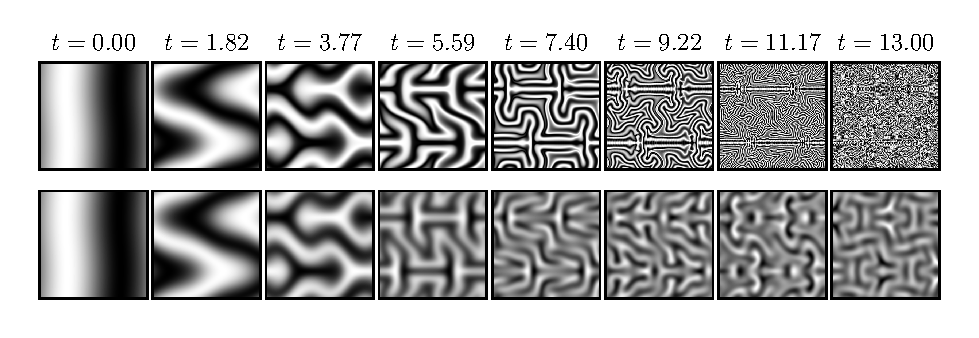
\includegraphics[width=6in]{ch-lit/images/enstrophy_film}}

% Optional, but recommended, Copyright page
\copyrightpage{Christopher J. Miles}

% Page numbering. If you don't include a frontispiece or copyright page, you'll need to change this for two-sided printing.
\makeatletter
\if@twoside \setcounter{page}{4} \else \setcounter{page}{1} \fi
\makeatother
 
% Optional Dedication page
\dedicationpage{ To my parents, teachers, and mentors who have provided encouragement throughout my life.}

% Optional Acknowledgements page
\startacknowledgementspage
I am greatly indebted to the mentors, instructors, departmental staff, friends, and family members who have supported me throughout my Ph.D. I am especially thankful for the mentorship of my advisor Charles Doering who  provided guidance throughout my studies. He has been a key element to my scientific and academic development. I would also like to gratefully acknowledge my committee members: Anthony Bloch, Jesse Capecelatro, Robert Deegan, and Mark Newman. Thank you for taking the time and effort to evaluate this work.

During my time at Michigan, I was fortunate to have many fruitful research discussions that impacted this work, especially those with Ian Tobasco, Karen Zaya, and Andre Souza. I also appreciate the helpful comments and feedback provided (some indirectly) on this work by Hongjie Dong, Luis Escauriaza, Guatum Iyer, Alexander Kiselev, Anna Mazzucato, and Christian Seis.

%I would like to thank Oliver Kripfgans who were involved in a M-Cubed collaborative research project on acoustic droplet vaporization (not included in this thesis) in my first half of my PhD. He and his lab members provided excellent guidance on conducting experiments. Thank you.
%
%I would like to give a special thanks to the Woods Hole Oceanographic Institution Geophysical Fluid Dynamics program which shaped my academic training during the summer of 2016. I was fortunate to work on active matter with Saverio Spagnolie and Michael Shelley who were great research mentors. Although this project does not appear in this thesis, this program definitely contributed to my academic development for which I am thankful.

Last but not least, I would like to sincerely thank Irene Park for always being supportive and caring throughout my graduate school years. She was always there for me and I am forever thankful. 
\label{Acknowledgements}

% Optional Preface page
%\startprefacepage
%\input{front-matter/preface}
%\label{Preface}

% Table of contents, list of figures, etc.
\tableofcontents     % Required
\listoffigures       % Required if there is more than one figure
%\listoftables        % Required if there is more than one table
%\listofmaps          % Required if there is more than one map
\listofappendices    % Required if there is more than one appendix
% \listofabbreviations % Optional. Abbreviations should be stored in a file named abbr.tex. Use ac{ } when referring to a particular acronym in text. For example, the tex file may read " \ac{MHD} is challenging field ..." and will appear in the PDF as "magnetohydrodynamic (MHD) is a challenging field..."  The first time you use an acronym, the full name of the acronym along with the acronym in brackets will be printed. If you specify the footnote option while loading the package, the full name of the acronym is printed as a footnote. The next time you access the acronym only the acronym will be printed. Note the acronym package does not support automatic capitalization at the beginning of sentences. A work around is to type in latex "Magnetohydrodynamic \acused{MHD} (\ac{MHD}) is a challenging field ... ".


% Optional in-dissertation Abstract Page
\startabstractpage
Mixing is a fundamental fluid mechanism that is crucial to the engineering of industrial processes within the chemical, pharmaceutical, petrochemical, food, and many other industries. Mixing is also important to areas of science including oceanography, turbulence, and atmospheric sciences. An important question to many domains is ``How does one mix efficiently?" We strive to make progress towards this question by studying a series of optimization problems on mixing. 

The first study presented is on optimization of a shell model of mixing. This model is based on a system of ordinary differential equations which mimic the time evolution of the Fourier spectrum of a dye concentration governed by the advection-diffusion equation. We investigate the local-in-time and global-in-time optimization within this model and show that mixing can be limited by diffusion. 

The second study investigates local-in-time optimization of the advection-diffusion partial differential equation. We demonstrate that many of the observations seen in the shell model extend to this setting such as evidence of a limitation on mixing by the inclusion of diffusion.

Lastly, we explore global-in-time optimization of the advection-diffusion equation. This last study is ongoing research at the moment: current results on this topic are presented and a comparison between local-in-time and global-in-time optimization is discussed. 
\label{Abstract}

\startthechapters 
% The individual files for each of the chapters are put here.
% Save each chapter of your thesis to a seperate tex file
% and then use the \input command to include this file in your
% thesis.  For instance you can save a file to "intro.tex" and 
% then type \input{intro}. 

 \chapter{Introduction}
 \label{chap:introduction}
 %%%
%%% 	CHAPTER: INTRODUCTION 
%%%

% OUTLINE


	% OPENING
	
\section{Why study fluid mixing?}			
		
Fluid mixing happens in a gust of wind and in a cup of morning coffee with cream. This phenomena is commonplace and plays an important role in many natural and engineering systems that humanity depends on. Our current lack of fundamental understanding of mixing impedes our ability to understand natural systems such as atmospheric and oceanic processes that impact our global climate. Mixing also serves as a key industrial process crucial for production within the food, chemical, pharmaceutical, and petrochemical industries. Thoughtful design of industrial mixing is essential for maximizing product yield and product quality throughout these industries. In addition, poor mixing design can come at a cost. In 1989, the cost of poor mixing was estimated to be \$1 -- \$10 billion US dollars in the chemical industry alone \cite{paul2004handbook}. Nearly everyone depends on these industries for basic household products, health needs, travel, and food. And in most situations, the cost in production is inevitably paid by consumers --- that includes you and me. 


Although mixing is highly prevalent and often utilized, its fundamental principles are still not fully known especially concerning how the interplay of advection and diffusion processes affect mixing rates and achievable filamentation length scales. To make progress on understanding the systems that involve mixing, we must understand mixing itself. Thus, the approach taken here is to study a theoretical and mathematical framework of mixing that has been stripped down to its essential elements. The perspective taken in this work is that one must understand the idealized problems first before tackling problems with added complexity. An idealized Carnot engine provides efficiency expectations of real-world heat engines each unique with its own complexity. By analogy,  we hope the idealized mixer presented here will provide theoretical principles on mixing efficiency about real-world mixers as well.


\section{What does well-mixed mean?}

\begin{figure}
	\centering
	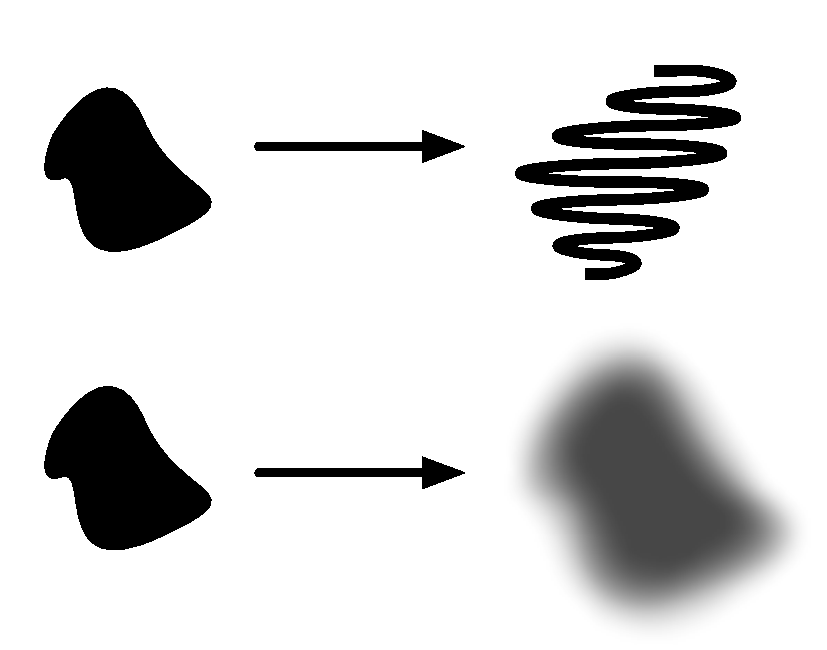
\includegraphics[width=0.7\textwidth]{ch-introduction/images/scale-and-intensity}
	\caption{Top transformation is a reduction in the scale of segregation. Bottom transformation is a reduction in the intensity of segregation}
	\label{fig:scale-and-intensity}
\end{figure}

In the pioneering work of P. V. Danckwerts (1952) \cite{Danckwerts1952}, the author identifies two indicators of mixed-ness: the scale of segregation and the intensity of segregation. The {\it scale of segregation } is the characteristic length scale present in the concentration. For instance, the process of thinning, elongating, and folding of a blob, as seen in the top graphic of figure \ref{fig:scale-and-intensity}, reduces the scale of segregation by creating a rich maze-like pattern with thin strands of dye.  The {\it intensity of segregation } refers to the variation of the concentration amplitude. This is naturally done by diffusion. The bottom graphic of figure \ref{fig:scale-and-intensity} shows a reduction in the overall variation and the concentration tends towards a state with a uniform concentration.





\section{Fluid mixing stages and mechanisms}

The seminal work of C. Eckart \cite{Eckart1948} describes the three stages of mixing:

\begin{enumerate}
\item {\it The initial stage}: The mixedness of the initial state will dictate the amount of `work' necessary to mix to a desired state. Typically, there will be large volumes of dye visible throughout the fluid.  Thus the preparation of the initial concentration is a stage in its own right before the fluid mechanisms are called into action.

\item {\it The intermediate stage}: {\it Advection}, or colloquially the act of stirring, will distort, stretch, and fold the volumes of dye to produce large gradients throughout the fluid and reduce the scale of segregation. 

\item {\it The final stage}: Lastly the gradients will disappear under the action of {\it diffusion}.  Diffusion refers to molecular diffusion throughout this work and not to be confused with its occasional usage of dispersal (to spread a dye thoughout space).  
\end{enumerate}
The intermediate and final stages are shown to happen sequentially in time. This is not completely accurate. These processes occur concurrently as we will investigate throughout this work.

In the stages above, we have introduced the two main mechanisms at play ---  advection and diffusion. Advection is a fluid mixing mechanism that when used appropriately can be an excellent way to reduce the scale of segregation. 

%Turbulent flows are commonly regarded as good mixers. In fact, its ability to mix may be considered a defining characteristic. To understand the impact of a turbulent flow on mixing, it is useful to examine the length scales present in the concentration field. This is commonly done through characterizing the scalar energy spectrum. The theory of Obukhoff (1949)\cite{Obukhov1949},  Corrsin (1951) \cite{Corrsin1951}, and Batchelor (1959)\cite{Batchelor1959a} captures the characteristics of the scalar energy cascades which have been verified numerically\cite{Eswaran1988,Holzer1994b,Shraiman2000a} and experimentally (CITATION). A key finding from their theory was the emergence of a length scale (now known as the Batchelor scale) where  advection and diffusion balance. The Batchelor scale is given by  $\ell_{b}= \sqrt{\kappa / \Gamma}$ where $\Gamma$ is the typical rate-of-strain of the fluid. For a turbulent flow to be sustained, there must be continual source of energy supplied to the fluid at the kinetic energy dissipation rate per unit mass $\epsilon$. This rate $\epsilon$ is related to the rate of strain $\Gamma = \langle |\nabla \mathbf{u}|^2 \rangle ^{1/2} $ by $\epsilon = \nu \Gamma^2$ where $\nu$ is the fluid viscosity \cite{Doering}. Using this relation, we find that the Batchelor scale is given by $\ell_{b}=\left(\frac{\kappa}{\nu}\right)^{1/2}\left(\nu^3/\epsilon\right)^{1/4}=S^{-\frac{1}{2}}\ell_{k}$ where $S=\frac{\nu}{\kappa}$ is the Schmidt number and  $\ell_{k}=\left(\nu^3/\epsilon\right)^{1/4}$ is the Kolmogorov length \cite{Dimotakis2005,Kolmogorov1941}.  The Batchelor scale defines the cutoff length in the scalar energy spectrum where there is rapid decay past this length according to the Obukhoff-Corrsin-Batchelor theory. Therefore, the presence of the Batchelor scale identifies a limit to the degree of mixing possible by a turbulent flow. 
	
\section{A mathematical framework for studying mixing}

The effect of advection and diffusion on the rate of fluid mixing depends on the particular mixing situation characterized by the unique fluid properties, specific mixing flow, and boundary geometry. In view of the vast complexity of the mixing situation, general principles of mixing underlying these various situations would be beneficial. In particular, it is valuable to determine how the mixing rate (typically the most optimal mixing rate) depends on aggregate flow intensity measures such as the stirring flows' energy and/or enstrophy. This is the objective of the research program encompassing many efforts \cite{CS2013,GI2014,JLT2012,JFM2011,  JLT2012, DF2014, GM2005,Yao2014a,JMP2012,Cortelezzi2008,Miles2018,Miles2017a} in last decade. 

With these goals in mind, a common approach taken throughout the literature is to consider the evolution of a tracer quantity $\theta$ advected by an incompressible ($\nabla \cdot\vec{u}=0$) flow $\vec{u}$ with mild physical constraints within a periodic box $D$ of side length $L$ in $d$ dimensions. All numerical simulations are done in 2 dimensions while analytical results are generally presented in arbitrary dimension. We will assume that $\theta$  has zero mean throughout this work. The tracer concentration field $\theta$ evolves according to the advection-diffusion equation,
\begin{equation}
	\label{eq:PDE_advection}
	\ppt{\theta}+\mathbf{u}\cdot \nabla \theta=\kappa \lap\theta,
\end{equation}
with initial data $\theta(\mathbf{x},0)=\theta_{0}(\mathbf{x})$, where $\kappa$ is the molecular diffusion coefficient and $\Delta = \nabla^2$ is the Laplacian operator. The flow intensity is constrained by enstrophy \begin{equation}
\ltwo{\nabla\u} = \sqrt{ \sint{|\nabla \mathbf{u}|^2} } =\Gamma L^{d/2}
\end{equation} or energy
\begin{equation} 
\ltwo{\u} = \sqrt{ \sint{| \mathbf{u}|^2} } = UL^{d/2}
\end{equation}
 where $\Gamma$ is the root mean square rate-of-strain and $U$ is the root mean square speed. We will also consider the time-average versions $\frac{1}{T}\int_0^T\ltwo{\nabla\u}^2 dt = \Gamma L^{d/2}$ or $\frac{1}{T}\int_0^T\ltwo{\u}^2 dt = U L^{d/2}$.


 The form above shows that the evolution of the tracer concentration $\theta$ is slaved to a given flow $\mathbf{u}$ which embodies, in many cases, most of the complexity of a particular mixing problem. The details of $\mathbf{u}$ alone can be complicated since in natural settings $\mathbf{u}$ is a solution of the Navier-Stokes equations. Although flow situations can be vastly different, they can still share commonalities such as incompressibility and similar amount of total energy or enstrophy. Note that enstrophy is proportional to the dissipation power for Newtonian fluids. We will only consider flows constrained by these properties for the purposes of simplicity and generality.


The negative Sobelov norms $H^{-n}$ \cite{GM2005, Mathew2007b,JLT2012, JFM2011} are measures of mixing used throughout the literature and the $H^{-1}$ norm (and sometimes referred to as the mix-norm) will be used here. The $H^{-n}$ norm for mean-zero scalar fields $\theta$ are given by  
%
\begin{equation}
\|\theta\|_{H^{-n}}=\ltwo{\nabla^{-n}\theta}=\sqrt{\sint{ |\nabla^{-n} \theta( \vec{x},t)|^2}}=\sqrt{ \sum_{\vec{k}\neq \vec{0}} L^d \frac{|\hat{\theta}_{\vec{k}}(t)|^{2}}{|\vec{k}|^{2n}}}
\end{equation}
%
where $\nabla^{-1}=\nabla \Delta^{-1}$, the operator $\Delta^{-1}$ acting on  a function $\rho$ returns the solution $\phi$ of the Poisson equation $ \Delta \phi = \rho $, and $\hat{\theta}_{\vec{k}}(t) =  \frac{1}{L^{d}}\sint{\theta(\vec{x},t)e^{-i\vec{k}\cdot\vec{x}}}$.  Lower values of the  $H^{-1}$ norm correspond to a more mixed state. Note that $H^{-1}$ norm can decrease in two ways. The first way is to decreasing the amplitudes of $|\hat{\theta}_{\vec{k}}|$ for $\vec{k}\neq 0$. This matches our first sense of mixing --- {\it homogenization}. The second way is by transferring spectral mass from the lower wave numbers to the higher wave numbers to take advantage of the $1/|\vec{k}|^2$ weighting of amplitudes at different length scales. This produces a scalar field with sharp gradients and small length scales which matches our second sense of mixing --- {\it filamentation}. Thus we can see that the $H^{-1}$ norm embodies both senses. 

The $L^{2}$ norm $\ltwo{\theta}$ defined by
%
\begin{equation}
\ltwo{\theta}=\sqrt{\sint{ | \theta( \vec{x},t)|^2}}=\sqrt{ \sum_{\vec{k}} L^d |\hat{\theta}_{\vec{k}}(t)|^{2}}
\end{equation}
%
and the $H^{1}$ norm $\hone{\theta}$ defined by 
%
\begin{equation}
\|\theta\|_{H^{1}} = \hone{\theta}=\sqrt{\sint{ |\nabla^{-1} \theta( \vec{x},t)|^2}}=\sqrt{ \sum_{\vec{k}} L^d |\vec{k}|^2|\hat{\theta}_{\vec{k}}(t)|^{2}}
\end{equation}
%
are also common measures of mixing and will be considered as well.  For those interested in other measures of mixing, see \cite{JLT2012}. 

			
\section{Pure diffusive mixing}
In the case without advection ($\vec{u}=\vec{0}$), equation \eqref{eq:PDE_advection} reduces to the classical heat equation \cite{Evans2010}. The Fourier modes evolve according to $\hat{\theta}_{\vec{k}}(t)=\hat{\theta}_{\vec{k}}(0)e^{-\kappa|\vec{k}|^2t}$. Thus we have explicit analytical results for the decay of the $H^{-1}$ norm by simply substituting this result. Note that $H^{-1}$ norm will surely decay monotonically since the amplitude of each mode does. Diffusion is unable to transfer spectral mass from the low wave number modes to the high wave number modes and thus is incapable of filamentation. Thus the pure diffusion case solely exploits homogenization. Also notice the unequal weighting attach to each mode. The Fourier modes with large wave number $|\vec{k}|$ decay at a much faster rate relative to the decay of those with small wave number.



\section{Pure advective mixing}
In the case without diffusion ($\kappa = 0$), pure advection of the flow is the only method of mixing, colloquially known as stirring. For a flow that is constrained by enstrophy, the mix-norm decays at most exponentially where the exponential rate is proportional to $\Gamma$ \cite{GI2014,CS2013}. This was mathematically proven by two separate approaches: G. Iyer {\it et. al.} \cite{GI2014} used regularization results of partial differential equations \cite{Crippa} while C. Seis \cite{CS2013} used methods from optimal transportation theory \cite{villani2003topics}. Furthermore, enstrophy-constrained flows that realize this exponential decay rate have been constructed analytically \cite{Alberti2014a}. On the other hand, energy-constrained flows can achieve even faster mixing rates. In fact they can achieve {\it perfect mixing in finite time} which means that the $H^{-1}$ norm reaches zero in finite time as opposed to approaching zero in infinite time as exhibited in the case for enstrophy-constrained mixing. This can be demonstrated by a `checkerboard' flow \cite{JMP2012} where the mix-norm achieves perfect mixing in finite time via linear decay.  For either flow intensity constraint, note that $H^{-1}$ norm decreases by exclusively exploiting filamentation without homogenization. This is exactly opposite to the purely diffusive case.

Many works \cite{DAlessandro1999a, Liu2006, Mathew2007b, Cortelezzi2008, DF2014, JFM2011, JMP2012, Farazmand, Balasuriya2005, Hobbs1998, Vikhansky2002} have framed mixing enhancement in terms of optimization and optimal control theory. Mathew {\it et al.} \cite{Mathew2007b} studied pure advection of a concentration field by a velocity field $\mathbf{u}=\sum_{i=1}^{N}\alpha_{i}\mathbf{u}_{i}$ where $\{\mathbf{u}_{i}\}$ is a finite set of divergence-free velocity fields and $\{\alpha_{i}\}$ is a set of time-dependent weights. The weights $\{\alpha_{i}\}$ were chosen to minimize the final-time $H^{-1/2}$ mix-norm subject to a fixed value of action or equivalently a fixed value of time-averaged energy. Necessary conditions for optimality were numerically solved by conjugate gradient. The authors considered two examples each using $\mathbf{u}_{1}$ and $\mathbf{u}_{2}$ as given cellular flow velocity fields. In both examples, they found that the $H^{-1/2}$ norm of the computed concentration field decayed at an exponential rate. Furthermore, the authors demonstrated that the kinetic energy must be conserved at all moments in time due to optimality conditions even though they only required that the {\it time-averaged} energy be fixed --- analogous results hold true in this work as well. For this particular choice of velocity fields, the enstrophy turns out to also be conserved. This is consistent with other theoretical and numerical works \cite{CS2013,GI2014,JFM2011,Alberti2014a} reporting exponential decay rates under fixed enstrophy.   

Cortelezzi {\it et al.} \cite{Cortelezzi2008} also considered controlling two given flows to enhance mixing. But rather than considering a superposition of two flows, the authors considered switching entirely between one flow and the other. In particular, the authors considered controls that picked one of two sine flows $\mathbf{u}_{1}=\sin(2\pi y)\hat{x}$ and $\mathbf{u}_{2}=\sin(2\pi x)\hat{y}$ at uniformly spaced switching times. The authors divided the optimization task into multiple optimization sub-problems performed over short time horizons covering the entire time interval. They found, in the presence and absence of diffusion, that the mixing efficiency, as measured by the $H^{-1/2}$ mix-norm, of the short-horizon optimization schemes was substantially better than the periodic control that alternates between the two flows at each switching time. They also concluded that mixing can be greatly enhanced when optimizing over very short time horizons.
 
 Lin {\it et al.} \cite{JFM2011} explored short-time considerations even further. They found an analytic expression for the instantaneous optimal choice of velocity field given the current concentration field under fixed energy and enstrophy constraints. This was done by minimizing the time derivative of the $H^{-1}$ norm at each instant. Using the resulting expression, they numerically integrated the advection equation forward in time while determining the optimal velocity field at each time step. For an enstrophy-constrained flow, they numerically demonstrated exponential decay of the $H^{-1/2}$ and $H^{-1}$ norms consistent with \cite{CS2013,GI2014,Alberti2014a,Mathew2007b}. Lunasin {\it et al.} \cite{JMP2012} also performed a similar analysis as Lin {\it et al.} for flows with fixed palenstrophy ($\|\Delta\mathbf{u}\|_{L^{2}}$). This form of optimization is referred to as local-in-time optimization and will be discussed further shortly.


\section{The interplay of advection and diffusion}

Finally, the case with diffusion and advection is the least explored in this framework and the focus of this thesis. It is known that the evolution of the $H^{-1}$ and $L^2$ norms decrease monotonically under the checkerboard flow introduced by \cite{JMP2012}
 while the $H^{1}$ increases until it reaches a peak and then decreases \cite{DF2014}. This peak corresponds to a  time when the length scales developed are small enough for diffusion to effectively act on steep gradients. In contrast to the `pure' cases mentioned earlier, it is important to note that the $H^{-1}$ can now decrease by the two avenues of homogenization and filamentation simultaneously. 

At this point, we can already see a glimpse of a conflict between diffusion and advection for the ultimate goal of optimal mixing. Pure advection succeeds at filamentation by transferring spectral mass from the low wave number modes to the high wave number modes in a continuous fashion. However in the presence of diffusion, a once optimal pure advection flow exceptional at filamentation will be met with potential conflict since homogenization by diffusion can stifle its progress in transferring spectral mass to high wave number modes. Given that diffusion is ubiquitous, we must come to terms with this conflict to produce efficient mixing.


		
\section{The question and goals}

In this work, the interplay of advection and diffusion is explored to determine its impact on the rate of mixing. As we have mentioned in the last section, there appears to be a conflict between advection and diffusion that arises when both are acting to reduce homogenization through reduction in scale and intensity of segregation simultaneously.  The main question underlying this entire thesis work is:

\begin{quote}
{\it What is the optimal mixing rate achievable under the enstrophy and energy constrained flows when both advection and diffusion are active? }
\end{quote}

We hope to make progress in answering this by posing the question as an optimization problem. We will consider the {\it local-in-time optimization} problem:

\begin{equation} 
\min_{\vec{u}} \ddt{}\hmone{\theta(\cdot, t) }^2
\end{equation}
where the flow intensity is constrained by enstrophy \begin{equation}
\ltwo{\nabla\u}^2 =\Gamma^2 L^{d}
\end{equation} or energy
\begin{equation} 
\ltwo{\u}^2 = U^2L^{d}.
\end{equation}
%
We also consider the {\it global-in-time optimization } problem:
%
\begin{equation} 
\min_{\vec{u}} \hmone{\theta (\cdot, T) }^2
\end{equation}
%
where the flow intensity is constrained by {\it time-averaged} enstrophy \begin{equation}
\frac{1}{T}\int_0^T\ltwo{\nabla\u}^2 = \Gamma^2 L^{d}
\end{equation} or time-averaged energy
\begin{equation} 
\frac{1}{T}\int_0^T \ltwo{\u}^2 = U^2L^{d}.
\end{equation}

For all formulations, the flow is always required to be divergence-free ($\nabla \cdot \mathbf{u} = 0$) and $\theta$ solves the advection-diffusion equation with initial data $\theta(\mathbf{x},0)=\theta_0(\mathbf{x})$.

%
%\section{Feasibility of optimal flows}
%
%It is natural to ask ``Are optimal flows as defined feasible?" and ``How would one generate such flows in reality?" The purpose of this study is not to tackle these questions directly since our formulation is not entirely suitable for these questions. The purpose of this study is to consider idealized mixing to provide expectations in the best-case scenario with absolute control over the velocity field under the assigned constraints. In reality absolute control is generally not obtainable. As mentioned in the Carnot engine analogy discussed earlier in this chapter, the Carnot engine is an idealized engine with efficiency expectations in the best-case scenario which bound realizable engines, the approach taken here is similar. We hope to construct idealized mixers with mixing efficiency exceptions that bound realizable flows with known flow intensities quantified by energy and enstrophy.
%
%Although we do not fully address feasibility in the series of studies presented here, we acknowledge that feasibility is an important issue and encourage research in this direction. We will however say as much as we can in this section on the topic of feasibility to promote investigation. 
%
%With the goal of feasibility in mind, we can work backwards from a desired flow $\mathbf{u}$ to obtain the required forcing $\mathbf{f}$ on a fluid. This  can be found by simply substituting a discovered (local- or global-in-time) optimal velocity field $\mathbf{u}$ into the Navier-Stokes equation:
%\begin{equation}
%\label{eq:ns}
%\mathbf{f} = \rho\partial_{t} \mathbf{u}  + \rho\mathbf{u}\cdot \nabla \mathbf{u} + \nabla p - \nu \Delta \mathbf{u} 
%\end{equation}
%where $\rho$ is the fluid density, $\nu$ is the viscosity, $p$ is the fluid pressure, and $\mathbf{f}$ is the required forcing. Thus, we have obtained the necessary forcing to generate the desired flow $\mathbf{u}$. The next natural question is ``How could you construct a mixing device to create the forcing $\mathbf{f}$?'' Although we do not provide an answer, the derived forcing $\mathbf{f}$ at least gives us a target to aim for when tasked with the engineering problem of designing a mechanical mixer that realizes the flow $\mathbf{u}$. 
%
%%Note that the power injected by external forcing on fluid is eventually exhausted by viscous dissipation in the fluid. The viscous power dissipation rate is $\nu\int_{D}|\nabla \mathbf{u}|^2 \, d\mathbf{x}$
%
%The required mechanical power and energy to operate a mixing device are also useful measures for evaluating feasibility. For instance if the mechanical power or energy blows up in finite time, this would rule out it feasibility. The mechanical power $P$ can be found by multiplying \eqref{eq:ns} by $\mathbf{u}$ and integrating over the domain $D$ to arrive at
% \begin{equation}
%(P \equiv ) \sint{\mathbf{f}\cdot\mathbf{u}} = \ddt{}\left( \frac{\rho}{2}\sint{|\mathbf{u}|^2}\right) + \nu\sint{|\nabla\mathbf{u}|^2}
%\end{equation}
%where the left-hand side is identified as the mechanical power $P$ injected into the fluid by the external forcing $\mathbf{f}$, $ \frac{\rho}{2}\sint{|\mathbf{u}|^2}$ is the total kinetic energy, and $\sint{|\nabla\mathbf{u}|^2}$ is the enstrophy. 
%
%
%Under the enstrophy-constrained case, we have
%\begin{equation}
%P = \ddt{}\left( \frac{\rho}{2}\sint{|\mathbf{u}|^2}\right) + \nu\Gamma^2 L^d.
%\end{equation}
%The associated mechanical energy $E = \int_0^{T} P(t) dt$ is 
%\begin{equation}
%E = \left( \frac{\rho}{2}\sint{|\mathbf{u}(\mathbf{x},T)|^2} - \frac{\rho}{2}\sint{|\mathbf{u}(\mathbf{x},0)|^2}\right) + \nu\Gamma^2 L^d T.
%\end{equation}
%By Poincare's inequality we find that 
%\[
%E \leq \frac{\rho}{4\pi}\Gamma^2L^{d+2}  + \nu \Gamma^2L^dT.
%\]
%Thus, we see that the mechanical power $P$ required over time depends on the rate of total kinetic energy associated with the flow $\mathbf{u}$. However, the total mechanical energy $E$ is guaranteed to stay bounded from above by a quantity linearly proportional to enstrophy quantified by $\Gamma^2 L^d$.  Although the construction of a mechanical mixer enforcing $\mathbf{f}$ remains a challenge, the amount of mechanical energy required to enforce the enstrophy constraint is sensible --- in the sense that the above energetic analysis does not rule out its physical feasibility (the mechanical energy $E$ does not diverge in time for instance). 
%
%
% Under the energy-constrained case, the mechanical power is
%\begin{equation}
%\label{eq:energy-power}
%P = \nu\sint{|\nabla\mathbf{u}|^2}
%\end{equation} 
%and the mechanical energy is
%\begin{equation}
%\label{eq:energy-energy}
%E = \nu\int_0^{T}\sint{|\nabla\mathbf{u}|^2}dt
%\end{equation} 
%Thus, the amount of mechanical power is proportional to the amount of enstrophy or viscous energy dissipation rate. The development of small length scales is not penalized under energy-constrained flows thus this could result in \eqref{eq:energy-power} growing over time. This will certainly be the case under the checkerboard flow without diffusion. In the case with diffusion, we will demonstrate in later chapters the presence of a limiting length scale in the concentration field $\theta$ proportional to a generalized Batchelor scale $\lambda_{U} = \frac{\kappa}{U}$. For the present analysis, note that it does not seem beneficial for mixing to generate length scales in the velocity field significantly smaller than those present in the concentration field.  If we assume that the Fourier spectrum is peaked around the wavenumber $\frac{2\pi}{\lambda_{U}}$ at later times after the developing the smallest length scale $\lambda_U$. Then, we hypothesize that, during this later stage, the mechanical power scales according to 
%\begin{equation}
%\label{eq:power-expectation}
%P \sim \nu \frac{(2\pi)^2}{\lambda_{B}^2}U^2 L^d  = \nu \frac{(2\pi)^2}{\kappa^2}U^4 L^d.
%\end{equation}
%Note the scaling with $\nu$, $\kappa$, and $U$. As $\kappa$ decreases, this increases the mechanical power. We will see in later chapters that a decrease in $\kappa$ is also accompanied by a beneficial {\it increase} in the mixing rate. Thus, this presents a trade off between these potential objectives: mixing efficiency and mechanical power. 
%
%In both enstrophy- and energy- constrained cases, it is beneficial to have a lower viscosity $\nu$. This is especially important for the energy-constrained case where the mechanical power is proportional to $\nu$.

\section{Organization of dissertation}
The rest of this dissertation is organized as follows:  Chapter \ref{chap:shellmodel} describes the local- and global-in-time optimization within the context of a shell model, a model representing the spectral dynamics of the advection-diffusion equation. Here we find the first indication that diffusion in some cases can penalize mixing performance. This work was published in the Journal of Nonlinear Science in 2017 \cite{Miles2017a}. Chapter \ref{chap:lit} studies local-in-time optimization in the context of the advection-diffusion partial differential equation. Here we investigate further the impact of diffusion. We find that diffusion can in some cases negatively impact the long-term mixing rate for local-in-time optimal flows. This work has been accepted for publication in Nonlinearity \cite{Miles2018}. Chapter \ref{chap:git} presents on-going work on global-in-time optimization of the advection-diffusion equation. An analytical result is presented showing that it is optimal to expend the stirring budget uniformly in time for the pure advection case. This result appears in an Appendix section of the 2017 Journal of Nonlinear Science article \cite{Miles2017a}.

%	
%	These problems are explored in the context of the shell model in chapter \ref{chap:shellmodel}. They are explored further in the context of the advection-diffusion equation in chapters \ref{chap:lit} and \ref{chap:git}.




% SCRATCHWORK BELOW

%Many have explored the idea of enhancing mixing by stirring.  Eckart (1948) is one of the earliest to explore this topic. He argued that there are three mixing stages: initial stage (persistance of large scales in initial concentration), intermediate stage (the creation of gradients induced by advection), and final stage (the disappearance of gradients by diffusion). He explored these phases in the simplified setting of a planar shear flow and concluded that the mixing times occurred on the order of $t=\ell^{2}/\kappa$ where $\ell$ is the length scale of the velocity field. Thus, Eckart was one of the first to quantify the impact of the velocity length scale on the concentration mixing rate.
%
%\section{turbulence}
%

%
%
%Mixing enhancement through optimization and optimal control techinques have been explored\cite{Mathew2007b,Cortelezzi2008,Liu2006, JFM2011}.

\chapter[Shell model]{Shell model \footnote{The content of this chapter has been published in the Journal of Nonlinear Science (2017) \cite{Miles2017a}.}}
% \chapter{Shell model}  \footnote{footnotes working fine}
\label{chap:shellmodel}
 


\section{Introduction}


Shell models are systems of ordinary differential equations that mimic the mathematical structure of the spectral representation of a partial differential equations \cite{PD2010}. They were introduced in the context of the Navier-Stokes equations to study turbulent cascade dynamics \cite{MHJ,Gledzer1973,Yamada1988a} while avoiding mathematical difficulties inherent in the full nonlinear partial differential equation. We provide a similar treatment of the advection and advection-diffusion equations in the context of transient mixing and use optimization techniques to study shell-model stirring strategies to optimally mix a tracer concentration.

The shell model is designed to show qualitative features of advection, notably conservation of the tracer density variance, i.e., the $L^2$ --- or more precisely $\ell^2$ --- norm of the tracer concentration. Mixing is quantified by a negative Sobolev norm, the $H^{-1}$ norm, for the tracer concentration, with a natural extension to the shell model, that can measure tracer dispersion even in the absence of diffusion. The shell model also displays quantitative correspondence with results for maximal mixing in the partial differential equation formulation including perfect (complete) mixing in finite time for sufficiently weak constraints on the stirring flow field and exponential decay of the mix-norm for other protocols. We extend the optimal stirring analysis to make predictions for the influence of diffusion on mix-norm decay.

This chapter is organized as follows. In Section \ref{sec:ashellmodel} we introduce the shell model. Local- and global-in-time optimization schemes are described in, respectively, Sections \ref{sec:LIT} and \ref{sec:GIT}. The two shell model stirring strategies are compared without diffusion in Section \ref{sec:nondiffusivecase}  and with diffusion in Section \ref{sec:diffusivecase}. The concluding section \ref{sec:discussion_shell} contains a discussion of the results. Appendix \ref{app:shellmodel} contains exact analytical results for a three-shell truncation and derivations of lower bounds on the mix-norm.

%In contrast to previous work,
%Foures {\it et al.}\cite{DF2014} considered controlling the initial velocity field and boundary conditions, for two-dimensional plane Poiseuille flow governed by full Navier-Stokes equations, rather than directly controlling the velocity field. The authors numerically studied the resulting advection and diffusion dynamics of the tracer concentration field due to the induced flow. The authors compared three objectives: optimization of energy, $H^{-1}$ mix-norm, and variance at the final time. They concluded that flows that optimized energy tended to be poor mixers relative to flows obtained by optimizing the $H^{-1}$ mix-norm and variance. 
%
%We are interested in making progress on the following two optimization formulations: 
%\begin{enumerate}
%	\item (Local-in-time optimization) What admissible velocity field produces the best instantaneous mixing rate?
%	That is, what flow field $\mathbf{u}(\mathbf{x}, t)$ realizes
%	\[
%		\min_{\mathbf{u}} \frac{d}{dt} \|\theta(\,\cdot\,,t)\|_{H^{-1}}^{2}
%	\]
%	at each instant of time $t$ subject to the enstrophy or energy intensity constraint. This is the question that Lin {\it et al.} \cite{JFM2011} studied in the partial differential equation setting without diffusion.
%
%	\item (Global-in-time optimization) What time-dependent velocity field will produce the most mixed state at a final time $T$? That is, what flow field $\mathbf{u}(\mathbf{x}, t)$, defined for $t \in [0,T]$, realizes
%	\[
%		\min_{\mathbf{u}}\|\theta(\,\cdot\, , T)\|_{H^{-1}}^{2}
%	\]
%	subject to either a {\it time-average} enstrophy constraint,
%	\[
%		\frac{1}{T}\int_{0}^{T}dt\int_{D}d^{d}\mathbf{x} \, |\nabla \mathbf{u}|^{2}= \frac{L^{d}}{\tau^{2}},
%	\]
%	or a time-average energy constraint,
%	\[
%		\frac{1}{T}\int_{0}^{T}dt\int_{D}d^{d}\mathbf{x} \, |\mathbf{u}|^{2}= U^{2}L^{d}.
%	\]
%\end{enumerate}
%The global-in-time optimization constraints allow the option of using the budget in a non-uniform fashion in time.  Global-in-time optimization, a full optimal control problem as formulated here, is still an open challenge with partial results provided by Mathew {\it et al.} \cite{Mathew2007b} and Cortellezi {\it et al.} \cite{Cortelezzi2008}. The proposed shell model agrees with the local-in-time optimization results at a qualitative level and provides new insights into the global-in-time optimization problem which will be the focus of future work. 
%

\section{A shell model}
\label{sec:ashellmodel}
Shell models are coarse-grain versions of the spectral representation of a partial differential equation. In particular the Fourier transform of the advection-diffusion equation (\ref{eq:PDE_advection}) becomes the infinite set of coupled ordinary differential equations
\begin{equation*}
	\partial_{t}\hat{\theta}(\mathbf{k},t)+i\sum_{j= 1,2,3}\sum_{\mathbf{k}'\in K}\hat{u}_{j}(\mathbf{k}-\mathbf{k}',t) \, k'_{j} \, \hat{\theta}(\mathbf{k}',t)+ \kappa \, |\mathbf{k}|^2\hat{\theta}(\mathbf{k},t)=0.
\end{equation*}


We course-grain this relation by `binning' the Fourier variables $\hat{\theta}(\mathbf{k},t)$ with wavenumbers $2^{n-1} k_{0}<|\mathbf{k}|<2^n k_{0} $ ($k_{0} = \frac{1}{2L}$) into a single variable $\theta_{n}(t)$ for $n=1,2, \dots ,\infty$. This binning process divides $\mathbf{k}$-space into concentric shells and hence the name---shell model. We similarly course-grain the Fourier amplitudes of the flow field $\hat{u}_{i}(\mathbf{k},t)$ into the variables $u_{n}(t)$ and look for the simplest shell model that retains mode-coupling between neighboring shells.
Thus, we choose the following form:
\begin{equation}
	\label{eq:shellNN_advection}
	\frac{d}{dt} \theta_{n}= k_{n-1}u_{n-1}\theta_{n-1}-k_{n}u_{n}\theta_{n+1} - \kappa \,  k_{n}^{2} \theta_{n}, \quad n=1,2,\dots,
\end{equation}
where $k_{n}=k_{0}2^{n}$ and $\theta_{0} \equiv 0 \equiv u_{0}$. $\kappa$ has units of $L^{2}/T$; $k_{n}$ has units of $1/L$; $u_{n}$ has units of $L/T$; and $\theta_{n}$ is unitless.
We may also consider $N$-shell truncated models with $n=1,2,\dots, N$ where $\theta_{n \ge N+1} = 0 = u_{n \ge N}$. See references \cite{MHJ,wirth1996,PD2010} for alternative shell models of advection-diffusion. 

This construction is not intended to be mathematically rigorous. Rather, it is meant to mimic the natural cascade of the spectrum of the tracer, progressively visiting each shell as stirring stimulates smaller length scales. Note that this model preserves the relation $\frac{d}{dt}\ltwo{\theta}^2 = -2\kappa \hone{\theta}^2$ (found by multiplying the advection-diffusion equation by $\theta$ and integrating over $D$), but now in an $l^{2}$ sense:
\begin{equation}
	\label{eq:shell_L2decay}
	\frac{d}{dt}\sum_{n=1}^{}\theta_{n}^2=- 2\kappa \sum_{n=1}^{}k_{n}^2\theta_{n}^2.
\end{equation}
It follows that the $l^{2}$ norm is conserved for the non-diffusive case.

Lastly, we define the $h^{\alpha}$ shell-model Sobolev norm as
\begin{equation}
	\|\psi(t)\|^2_{h^{\alpha}} \equiv \sum_{m=1}^{} k_{m}^{2\alpha}\psi^{2}_{m}(t).
\end{equation}
for any vector $\psi = (\psi_{1}, \psi_{1}, \dots)$. The shell-model $h^{-1}$ mix-norm is defined as $\| \theta (t) \|_{h^{-1}}$. We denote the intensity constraints of the shell-model flow in terms of $\| u (t) \|^{2}_{h^{\alpha}}$. When $\alpha=0$ this is the $\ell^2$ analog of the energy and $\alpha=1$ returns an expression for enstrophy. The norm operator  $\|\cdot\|_{h^{\alpha}}$ has units of $L^{-\alpha}$.

\section{Instantaneous optimization}
\label{sec:LIT}

We begin by asking, ``What admissible control will produce the best instantaneous mixing rate?'' The analysis shown here parallels the work done by Lin {\it et al} \cite{JFM2011} in the partial differential equation setting. We formulate this question as the following: find the $u$ that realizes
\begin{equation}
	\label{eq:shellNN_lit_prob}
	\min_{u}  \frac{d}{dt} \| \theta (t) \|^{2}_{h^{-1}}
\end{equation} at each time $t$ subject to the constraint
\begin{equation}
	\label{eq:shellNN_lit_contstraint}
	\| u (t) \|_{h^{\alpha}} =W^{(\alpha)}
\end{equation}
where $W^{(0)}=U$ (energy) and $W^{(1)}=1/\tau$ (enstrophy). The root-mean-square rate-of-strain $\Gamma$ is given by $\Gamma = 1/\tau$.

Differentiating the mix-norm and using (\ref{eq:shellNN_advection}), we find
\begin{equation}
	\label{eq:deriv_mix_norm}
	\frac{d}{dt} \| \theta (t) \|^{2}_{h^{-1}} = 2 \sum_{n=1}  \left(k_{n+1}^{-2}-k_{n}^{-2}\right)\theta_{n}\theta_{n+1}k_{n}u_{n} - \kappa \,  \theta_n^2
\end{equation}
and the optimization problem is solved by the method of Lagrange multipliers. The solution is
\begin{equation}
	\label{eq:LIT_optimal}
	u_{n}^{(\alpha)}(t) =-\frac{W^{(\alpha)}\gamma^{(\alpha)}_{n}(t)}{k^{\alpha}_{n}\|\gamma^{(\alpha)}(t)\|_{l^{2}}}
\end{equation}
where $ \gamma^{(\alpha)}_{n}(t) \equiv (k_{n+1}^{-2}-k_{n}^{-2})k_{n}^{1-\alpha} \, \theta_{n}(t) \, \theta_{n+1}(t)$ --- at least, when $\|\gamma^{(\alpha)}(t)\|_{l^{2}} \neq 0$.

An alternative stategy is needed when $\|\gamma^{(\alpha)}(t)\|_{l^{2}} = 0$. An analgous situation arises in the partial differential equation setting \cite{JFM2011} and the second derivative $ \frac{d^{2}}{dt^2} \| \theta (t) \|^{2}_{h^{-1}} $ is minimized instead at these instances. We will do the same here. We write the second derivative as
\begin{equation}
	\label{eq:LIT_2derivative}
	\frac{d^{2}}{dt^2} \| \theta (t) \|^{2}_{h^{-1}} =u^{T}Bu+c^{T}u+d
\end{equation}
where
\[
	B_{nm}\equiv\left\{
	\begin{array}{cl}
		2(k_{n+1}^{-2}-k_{n}^{-2})k_{n}^{2}(\theta_{n}^{2}-\theta_{n+1}^{2}) & m=n              \\
		-2(k_{n+1}^{-2}-k_{n}^{-2})k_{n}k_{n+1}\theta_{n}\theta_{n+2}        & m=n+1            \\
		2(k_{n+1}^{-2}-k_{n}^{-2})k_{n}k_{n-1}\theta_{n-1}\theta_{n+1}       & m=n-1            \\
		0                                                                    & \mbox{otherwise}
	\end{array}
	\right. ,
\]
\[
	c_{n} = -2\kappa \, (k^{-2}_{n+1}-k^{-2}_{n})(k_{n+1}^{2}+k_{n}^{2})k_{n}\theta_{n}\theta_{n+1} ,
	\qquad \text{ and } \qquad
	d=\sum_{n=1} 4 \kappa^2 \, k_{n}^{2}\theta_{n}^{2}.
\]
We want to find the minimum of (\ref{eq:LIT_2derivative}) subject to the intensity constraint (\ref{eq:shellNN_lit_contstraint}).
By the method of Lagrange multipliers, the optimizer satisfies the following system of equations:
\begin{IEEEeqnarray}{rCl}
	\label{eq:system_of_equations}
	\left(B^{T}+B-\lambda K^{(\alpha)} \right) \,u & = & -c \IEEEyesnumber\IEEEyessubnumber* \\
	\|u\|_{h^{\alpha}}& = &  W^{(\alpha)}
\end{IEEEeqnarray}
where $\lambda$ is a lagrange multiplier and $K^{(\alpha)}=\mbox{diag}(k_{1}^{2\alpha}, \dots, k_{N-1}^{2\alpha})$. The general local-in-time strategy is to minimize the $(n+1)$th time derivative of $\|\theta(t)\|_{h^{-1}}$ if the control $u$ does not affect the $1$st through $n$th derivatives. We will soon return to the local-in-time strategy when applying it in sections \ref{sec:nondiffusivecase} and \ref{sec:diffusivecase}.

\section{Global-in-time optimization}
\label{sec:GIT}
Let's explore the global-in-time strategy which optimizes mixing at the end time rather than instantaneously. In this case we wish to solve the following global-in-time optimization problem: at some final time $T > 0$ find
\begin{equation}
	\label{eq:shellNN_git_probM}
	\min_{u}  \| \theta (T) \|^{2}_{h^{-1}} 
\end{equation}
subject to the time averaged intensity constraint
$
\frac{1}{T}\int_{0}^{T}\| u (t) \|^{2}_{h^{\alpha}}\: dt = [W^{(\alpha)}]^2.
$
Toward this end we introduce the augmented Lagrangian
\begin{multline*}
	\mathcal{ L} \{ \theta, u,\phi,\mu \} = \frac{1}{2} \sum_{n=1}^{}\frac{\theta_{n}^{2}(T)}{k_{n}^2} + \int_{0}^{T}\Bigg \{\sum_{n=1}^{}\phi_{n}\left(k_{n-1}u_{n-1}\theta_{n-1}-k_{n}u_{n} \theta_{n+1}- \kappa k_n^2 \theta_n -\dot{\theta}_{n}\right) \\
	+  \frac{\mu }{2}\left( \sum_{n=1}^{}k_{n}^{2\alpha}u_{n}^{2} - [W^{(\alpha)}]^2\right)  \Bigg\}\: dt
\end{multline*}
where for truncated shell models the first two sums above run up to $n=N$ while the third terminates at $N-1$. At extrema the first variations vanish with respect to the variables $\theta, \phi, u$ and $\mu$:

\begin{subequations}
	\label{eq:first_variation}
	\begin{align}
		\frac{\delta \mathcal{L}}{\delta \theta_{n}(T)}&=0  \Rightarrow & \frac{\theta_{n}(T)}{k_{n}^2}-\phi_{n}(T)&=0
		\label{eq:first_variation_terminal} \\
		\frac{\delta \mathcal{L}}{\delta \theta_{n}}&=0  \Rightarrow  & \dot{\phi}_{n}- k_{n-1}u_{n-1}\phi_{n-1} + k_{n}u_{n} \phi_{n+1} - \kappa \, k_n^2\phi_n &=0
		\label{eq:first_variation_adjoint} \\
		\frac{\delta \mathcal{L}}{\delta \phi_{n}}&=0  \Rightarrow  & \dot{\theta}_{n}- k_{n-1}u_{n-1}\theta_{n-1} + k_{n}u_{n} \theta_{n+1} + \kappa \, k_n^2\theta_n &=0
		\label{eq:first_variation_state} \\
		\frac{\delta \mathcal{L}}{\delta u_{n}}&=0 \Rightarrow  &  k_{n}\phi_{n+1}\theta_{n} - k_{n}\phi_{n}\theta_{n+1}+\mu k_{n}^{2\alpha}u_{n} &=0
		\label{eq:first_variation_optimality} \\
		\frac{\delta \mathcal{L}}{\delta \mu}&=0 \Rightarrow &
		\frac{1}{T}\int_{0}^{T}\| u (t) \|^{2}_{h^{\alpha}}\: dt - [W^{(\alpha)}]^2 &= 0
		\label{eq:first_variation_constraint}
	\end{align}
\end{subequations}
Thus, (\ref{eq:first_variation}) holds true for all extrema of the augmented Lagrangian and therefore gives necessary conditions for a global optimizer. 


 For the non-diffusive case, an explicit calculation of the time derivative of $\| u(t)\|_{h^{\alpha}}$ reveals that $\| u(t)\|_{h^{\alpha}}$ is conserved for an optimal trajectory by making use of (\ref{eq:first_variation}) as done in Appendix \ref{appendix:budget_conservation}. This is interesting, since we only demanded that the {\it time-average} of stirring strength be fixed and equal to $W^{(\alpha)}$. An analogous statement holds in the context of the partial differential equation as well (see Chapter \ref{chap:git}) which is an extension of the results first demonstrated by Mathew {\it et al} \cite{Mathew2007b}. The theory developed here will be applied to various cases in the next two sections.


\section{Mixing without diffusion}
\label{sec:nondiffusivecase}

We will first consider the local-in-time strategy starting from the most unmixed state. Then we study the three-shell truncated model which demonstrates the difference between local-in-time and global-in-time strategies. Lastly before introducing diffusion, we will show that the key features of global-in-time optimization shown in three-shell truncated model carry over naturally to models with a larger number of shells.

\subsection{Local-in-time strategy for infinite system}
\label{sec:LIT_MUIC}


Consider the enstrophy-constrained case and start the infinite system with the most unmixed possible state, $\theta(0)=(1, 0 , 0 \dots)^{T}$.  The local-in-time strategy uses each component of the control vector $u$ sequentially and in a piecewise fashion over time. We segment time into intervals, $[t_{n},t_{n+1}]$, of equal duration where $t_{n}= \frac{ \tau (n-1) \pi }{2} $ is the time when the state vector is entirely in the $n$th shell ($\theta_n =1$ and $\theta_{m\neq n}=0$). More precisely for $t\in
[t_{n},t_{n+1}]$, the optimal control is  $u_{n}= \frac{1}{\tau k_{n}}$ and $u_{m\neq n} =0$ while the state vector is given by $\theta_{n}(t) =\cos ((t - t_{n})/\tau)$ and $\theta_{n+1}(t) = \sin ((t - t_{n})/\tau) $ and all other components of $\theta$ are identically zero. The local-in-time strategy is shown graphically in figure \ref{fig:lit_muic}. We find that the mix-norm evaluated at times $t_{n}$ falls off exponentially;  Given that $\| \theta (t_{n}) \|^{2}_{h^{-1}}=\frac{1}{2 k_{n}^{2}}=\frac{1}{2  \, 2^{2n-2}}$ and using the relation $t_{n}= \frac{ \tau (n-1) \pi }{2} $ , we find that
\begin{equation}
	\| \theta (t_{n}) \|_{h^{-1}}=\| \theta (0) \|_{h^{-1}}\exp(- \log(2) t_{n} /\pi \tau).
\end{equation}
We highlight that this exponential decay agrees qualitatively with known results on the mixing rate with the enstrophy constraint \cite{GI2014,CS2013,JFM2011,Alberti2014a, Yao2014a}. In fact it can be shown definitively that the mix-norm decays no faster than exponentially. More precisely, (see Appendix \ref{appendix:lower_bound_enstorphy_nodiff} for derivation)
\begin{equation}
	\label{eq:bound_enstrophy_no_diff_main_text}
	\| \theta (t) \|_{h^{-1}} \geq \|\theta (0)\|_{h^{-1}} \exp \left( - \frac{3t}{2\tau} \right)
\end{equation}
for {\it every} stirring strategy.
The local-in-time strategy is illustrated in figure \ref{fig:lit_muic} and compared to this bound (\ref{eq:bound_enstrophy_no_diff_main_text}).

For the energy-constrained case, we again segment time into intervals $[t_{n},t_{n+1}]$ which are geometrically decreasing in duration where the times  $t_{n}$ are defined by $t_{n+1}= t_{n}+\Delta t_{n}$, $t_{1}=0$, and $\Delta t_{n}= \frac{ \pi }{2Uk _{n}} $. During each interval $[t_{n},t_{n+1}]$, the control is given by $u_{n}= U$ and $u_{m\neq n} = 0$ while the state vector is given by $\theta_{n}(t) =\cos (k_{n} U (t - t_{n}))$ and $\theta_{n+1}(t) = \sin (k_{n} U (t - t_{n})) $. Therefore the solution is similar to the enstrophy-constrained case except now the intervals are shrinking at a geometric rate. Thus the mix-norm goes to zero ($\lim_{n\rightarrow \infty} \| \theta (t_{n}) \|_{h^{-1}}= \lim_{n\rightarrow \infty} \frac{1}{k_{n}} =0$) in finite time since
\begin{equation}
	(t_{\infty}\equiv) \lim_{n \rightarrow \infty} t_{n} = \sum_{n=1}^{\infty} \Delta \tau_{n} =  \frac{ \pi }{2k_{0} U}.
\end{equation}
Note that if the entire concentration starts in the $m$th shell ($\theta(0)=\mathbf{e}_{m}$), then $t_{\infty}$ becomes the partial sum $t_{\infty}=\sum_{n=m}^{\infty}\Delta \tau_{n}$.  Once more we get qualitative agreement with known results from fluid mixing. Lunasin {\it et al} \cite{JMP2012} showed that perfect mixing in finite time for a simple binary distribution with fixed energy is indeed possible. 

We also obtain a lower bound for the energy-constrained case: (see derivation in Appendix \ref{appendix:bound_energy_no_diff})
\begin{equation}
	\label{eq:bound_energy_no_diff_main_text}
	\|\theta (t) \|_{h^{-1}} \geq\|\theta (0) \|_{h^{-1}}(1 -t/t_c)
\end{equation}
where $t_{c}=\frac{2}{3U}\frac{\|\theta(0)\|_{h^{-1}}}{\|\theta (0) \|_{l^{2}}}$. Figure \ref{fig:lit_muic} shows the local-in-time strategy for this case compared to the bound (\ref{eq:bound_energy_no_diff_main_text}) shown above.

In either constraint, the state vector moves from plane to plane. The state vector first rotates in the $\theta_{1}$-$\theta_{2}$ plane from the $\theta_{1}$ axis to the $\theta_{2}$ axis and then rotates in the $\theta_{2}$-$\theta_{3}$ plane from the $\theta_{2}$ axis to the $\theta_{3}$ axis and so forth. Note that for this particular initial condition, the analysis holds for $N$-shell truncated models and the above strategy holds for times $t < t_{N}$. When $t=t_{N}$, the state vector has reached the final shell and it is no longer possible to decrease the mix-norm any further.  Note that the local-in-time strategy behaves somewhat like a discrete analog to the self-similar strategies \cite{Alberti2014a,Yao2014a} found in the continuous partial differential equation problem since the same transformation is applied sequentially at piecewise time intervals at smaller and smaller scales.


\begin{figure*}[!ht]
	\centering
	\includegraphics[width=1.0\textwidth]{ch-shellmodel/images/lit_muic}
	\caption{Local-in-time strategy without diffusion starting initially from the most unmixed state. The entrophy-constrained case ($\frac{1}{\tau}=1$) is shown on the left subplots where (A) shows the state, (B) shows the control, and (C) shows the mix-norm. The energy-constrained case ($U=1$) is shown on the right subplots where (D) shows the state, (E) shows the control, and (F) shows the mix-norm. }
	\label{fig:lit_muic}
\end{figure*}



\subsection{Global-in-time strategy for 3-shell truncated model with enstrophy constraint}
\label{sec:git_enstrophy_3shell}

The diffusionless 3-shell truncated model, given by 
\begin{equation}
	\label{eq:3_mode_state}
	\left(
	\begin{array}{c}
		\dot{\theta}_{1} \\
		\dot{\theta}_{2} \\
		\dot{\theta}_{3}
	\end{array}
	\right)
	=\underbrace{ \left(
		\begin{array}{ccc}
			0          & -k_{1}u_1 & 0         \\
			k_{1}u_{1} & 0         & -k_{2}u_2 \\
			0          & k_{2}u_2  & 0
		\end{array}
		\right)}_{\equiv A(t)}
\left(
\begin{array}{c}
	\theta_{1} \\
	\theta_{2} \\
	\theta_{3}
\end{array}
\right),
\end{equation}
is the simplest reduced model that retains many interesting features of the full infinite system. From the last section, we know that the local-in-time strategy is to move along planes one by one. This holds for the 3-shell truncated model as well. 

Now, let us determine how you can improve upon the local-in-time strategy by considering the global-in-time strategy. We would like to minimize
$\| \theta (T) \|^{2}_{h^{-1}}$ subject to the enstrophy constraint, $\frac{1}{T}\int_{0}^{T}\| u(t)\|^{2}_{h^{1}} dt =  \frac{1}{\tau^2}.$ It is shown in Appendix \ref{appendix:oc3tm} that the solution to (\ref{eq:first_variation}) for $N=3$ has the following form: 
\begin{equation}
	\label{eq:3_shell_optimal_control}
	k_{1}u_{1}=\frac{1}{\tau} \cos(\omega t) \qquad \text{ and } \qquad k_{2}u_{2}=\frac{1}{\tau} \sin(\omega t)
\end{equation}
where $\omega$ is a real number left to be determined. To help determine the solution to (\ref{eq:3_mode_state}) given this optimal control (\ref{eq:3_shell_optimal_control}), we  decompose $A$ as
$A=k_{2}u_{2}S_{x}+k_{1}u_{1}S_{z}= \vec{B}\cdot\vec{S} $
where $\vec{B}=[k_{2}u_{2}, 0, k_{1}u_{1} ]$ and  $\vec{S}=[S_{x},S_{y},S_{z}]$ whose elements are a common choice of basis for $\mathbf{so}(3)$ given by
\[
	S_{x}=\left(
	\begin{array}{ccc}
		0 & 0 & 0  \\
		0 & 0 & -1 \\
		0 & 1 & 0
	\end{array}
	\right)
	\quad
	S_{y}=\left(
	\begin{array}{ccc}
		0  & 0 & 1 \\
		0  & 0 & 0 \\
		-1 & 0 & 0
	\end{array}
	\right)
	\quad
	S_{z}=\left(
	\begin{array}{ccc}
		0 & -1 & 0 \\
		1 & 0  & 0 \\
		0 & 0  & 0
	\end{array}
	\right).
\]
Notice that these elements satisfy the following commutation relations: $ [S_{x},S_{y}]=S_{z} ,  [S_{y},S_{z}]=S_{x}$, and  $[S_{z},S_{x}]=S_{y}. $
Given the above reformulation,  we arrive at
\begin{equation}
	\frac{d}{dt}\theta= \vec{B}\cdot\vec{S} \, \theta
\end{equation}
which is similar to the Schr\"odinger equation for a magnetic field-spin interaction. In this view the optimal solution behaves like a rotating magnetic field as seen in nuclear magnetic resonance. As a result this system `maps' to a two-state spin system coupled with a driven oscillatory magnetic field \cite{Feynman2010,Shankar1994,Sakurai1995}. We adapt well-known techniques \cite{rabi1954} from this area to arrive at the solution (see Appendix \ref{appendix:ss3tm})
\begin{equation}
	\theta(t)=\exp(\omega t S_{y})\exp\left(-\omega t S_{y}+\frac{t}{\tau}  S_{z}\right)\theta(0)
\end{equation}
or rewritten as \cite{SLA2005}
\begin{equation}
	\label{eq:3_shell_state_solution}
	\theta(\omega  ,\tau, t)=
	\left(
	\begin{array}{c}
		\cos(\omega t) \cos(\nu t) + \frac{\omega}{\nu} \sin(\omega t) \sin(\nu t)  \\
		\frac{1}{\nu\tau}  \sin(\nu t)                                              \\
		-\sin(\omega t) \cos(\nu t) + \frac{\omega}{\nu} \cos(\omega t) \sin(\nu t) \\
	\end{array}
	\right)
\end{equation}
where $\nu=\sqrt{\omega^{2}+\frac{1}{\tau^{2}}}$. Given the end condition  $\phi_{n}(T)=\theta_{n}(T)/k_{n}^{2}$ and the optimality condition (\ref{eq:first_variation_optimality}), we arrive at the system of nonlinear equations:
\begin{subequations}
	\label{eq:nonlinear_system}
	\begin{align}
	F_{1}\left(\omega , \mu ; \tau , T \right) &\equiv \mu \frac{T}{\tau}\cos(\omega T)  - \left(\frac{1}{k_{1}^2}-\frac{1}{k_{2}^2}\right) \theta_{1}\left(\omega ,\tau,T\right)  \theta_{2}\left(\omega ,\tau,T\right)=0\\
	F_{2}\left(\omega , \mu ;  \tau , T \right)  &\equiv \mu \frac{T}{\tau} \sin(\omega T) -  \left(\frac{1}{k_{2}^2}-\frac{1}{k_{3}^2}\right)\theta_{2}\left(\omega ,  \tau ,T\right)  \theta_{3}\left(\omega ,  \tau ,T\right)=0 .
	\end{align}
\end{subequations}

\begin{figure*}[!ht]
	\centering
	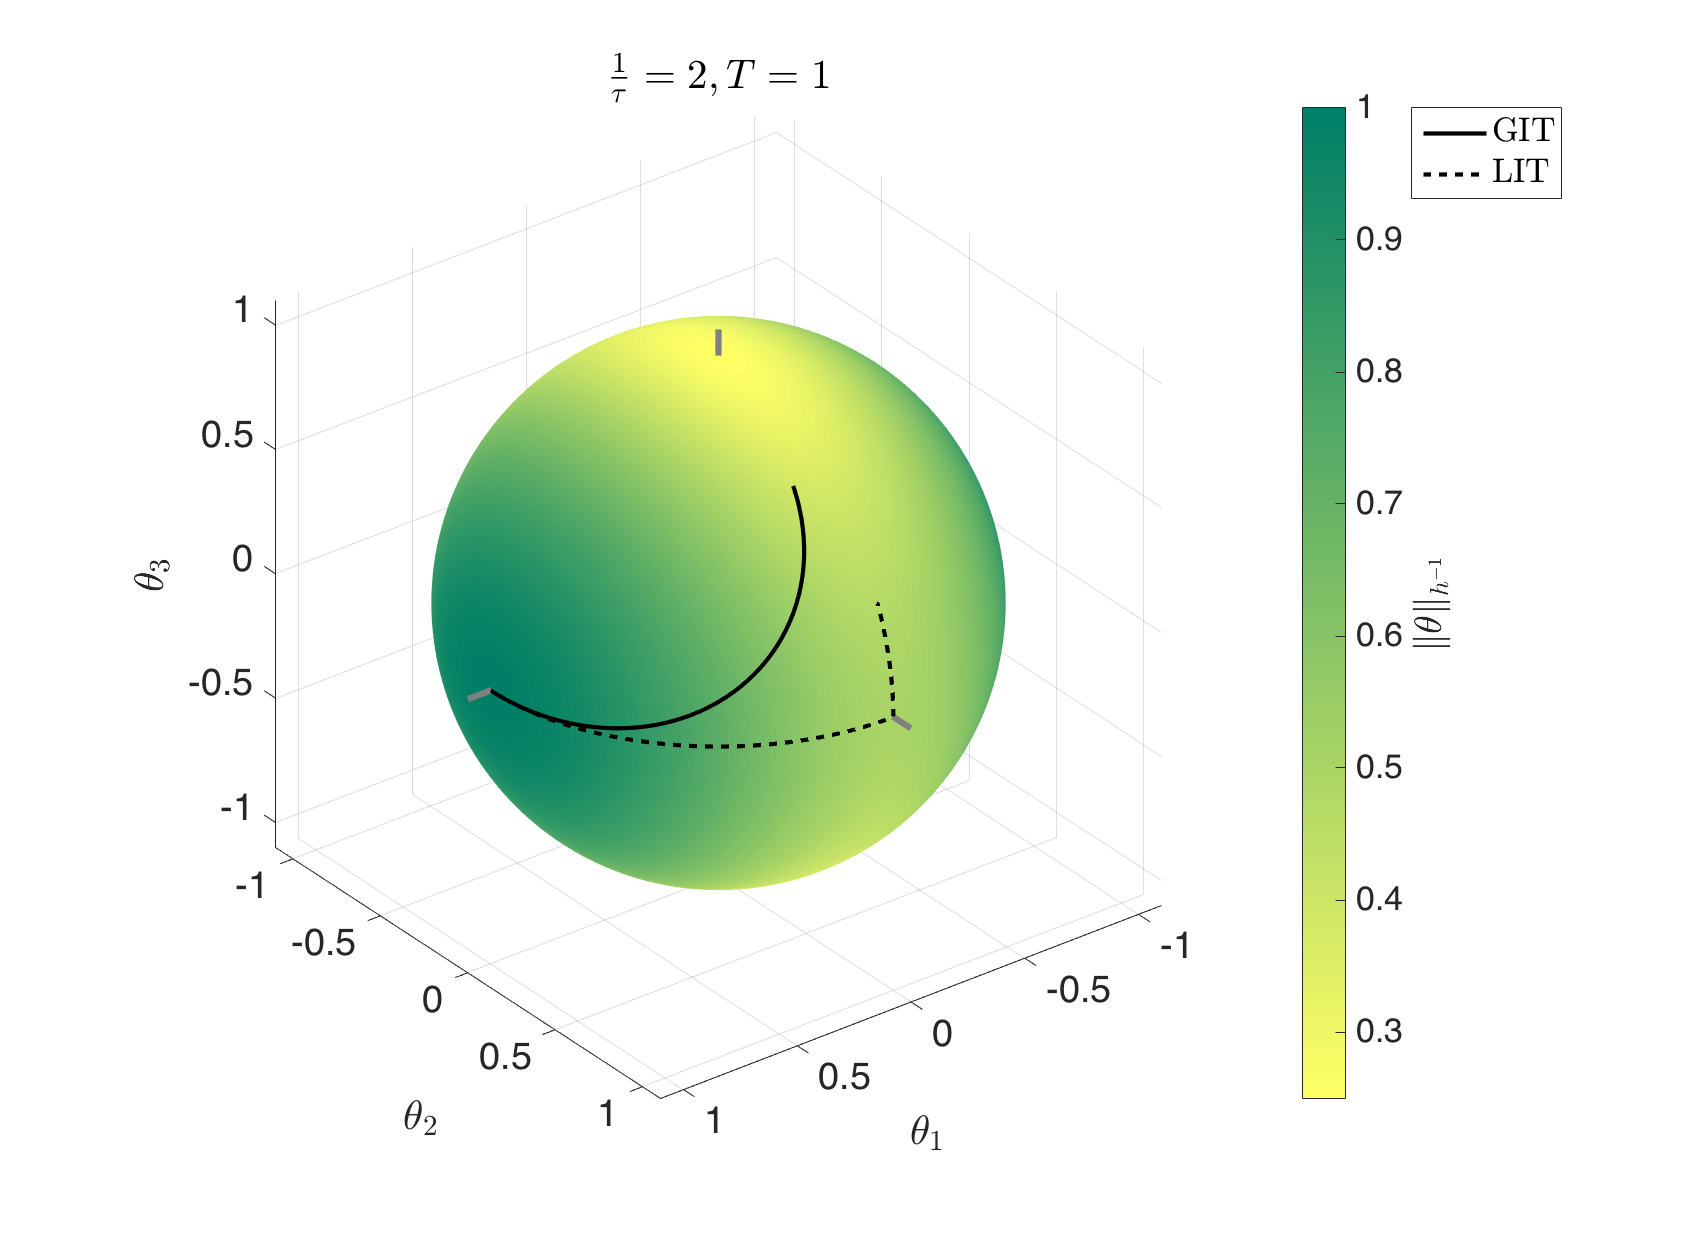
\includegraphics[width=0.7\textwidth]{ch-shellmodel/images/trajectories}
	\caption{Global-in-time and local-in-time trajectories for 3-shell model with $\frac{1}{\tau}=2$ and $T=1$ confined to a sphere with a radius given by the conserved quantity $\|\theta\|_{l^{2}}$. The color indicates the degree of mixing quantified by the mix-norm $\|\theta\|_{h^{-1}}$. }
	\label{fig:trajectories}
\end{figure*}

Using parameters $1/\tau = 2$ and $T=1$, we numerically computed $\omega \approx 1.249$ from (\ref{eq:nonlinear_system}). Thus, (\ref{eq:3_shell_optimal_control}) and (\ref{eq:3_shell_state_solution}) are known functions of time. With these parameters, the local-in-time and global-in-time trajectories evolve on a sphere with a radius defined by $\|\theta(0)\|_{l^{2}}$ in $\theta$-state space. And, the global-in-time strategy `takes a shortcut' past the $\theta_{2}$ axis relative to the local-in-time strategy as shown in figure \ref{fig:trajectories}. This short-cutting feature generalizes to truncated shell models with larger $N$ as shown in the next section.

When $ \frac{1}{\tau} =\frac{1}{\tau^{*}}\equiv\frac{\sqrt{3}\pi }{2T} $, the optimal control is given by
\begin{equation}
	\label{eq:proposed_control}
	k_{1}u_{1}=\frac{1}{\tau^{*}}\cos(\omega^{*} t) \quad
	k_{2}u_{2}=\frac{1}{\tau^{*}}\sin(\omega^{*} t).
\end{equation}
where  $\omega^{*}=\frac{\pi}{2T}$. (\ref{eq:proposed_control}) satisfies the budget constraint. This form is again the same as (\ref{eq:3_shell_optimal_control}) and therefore the state vector solution is given by (\ref{eq:3_shell_state_solution}) with $\frac{1}{\tau}=\frac{1}{\tau^{*}}$ and $\omega =\omega^{*}$. By evaluating (\ref{eq:3_shell_state_solution}) at $t=T$, we find that $\theta(T) = (0, 0, 1)^{T}$ which is the most mixed state. Therefore the proposed control (\ref{eq:proposed_control}) is a {\it global } optimum. The parameter regime with $\frac{1}{\tau}> \frac{1}{\tau^{*}}$ is not of interest since this corresponds to having excess budget. To handle this situation, introduce an inequality rather than equality in our budget constraint. If this change is made, (\ref{eq:proposed_control}) would be the optimal solution for all values $\frac{1}{\tau}> \frac{1}{\tau^{*}}$.

\subsection{Global-in-time strategy for N-shell truncated models}
\label{sec:ND_GIT_Nshell}
\begin{figure*}[!ht]
	\centering
	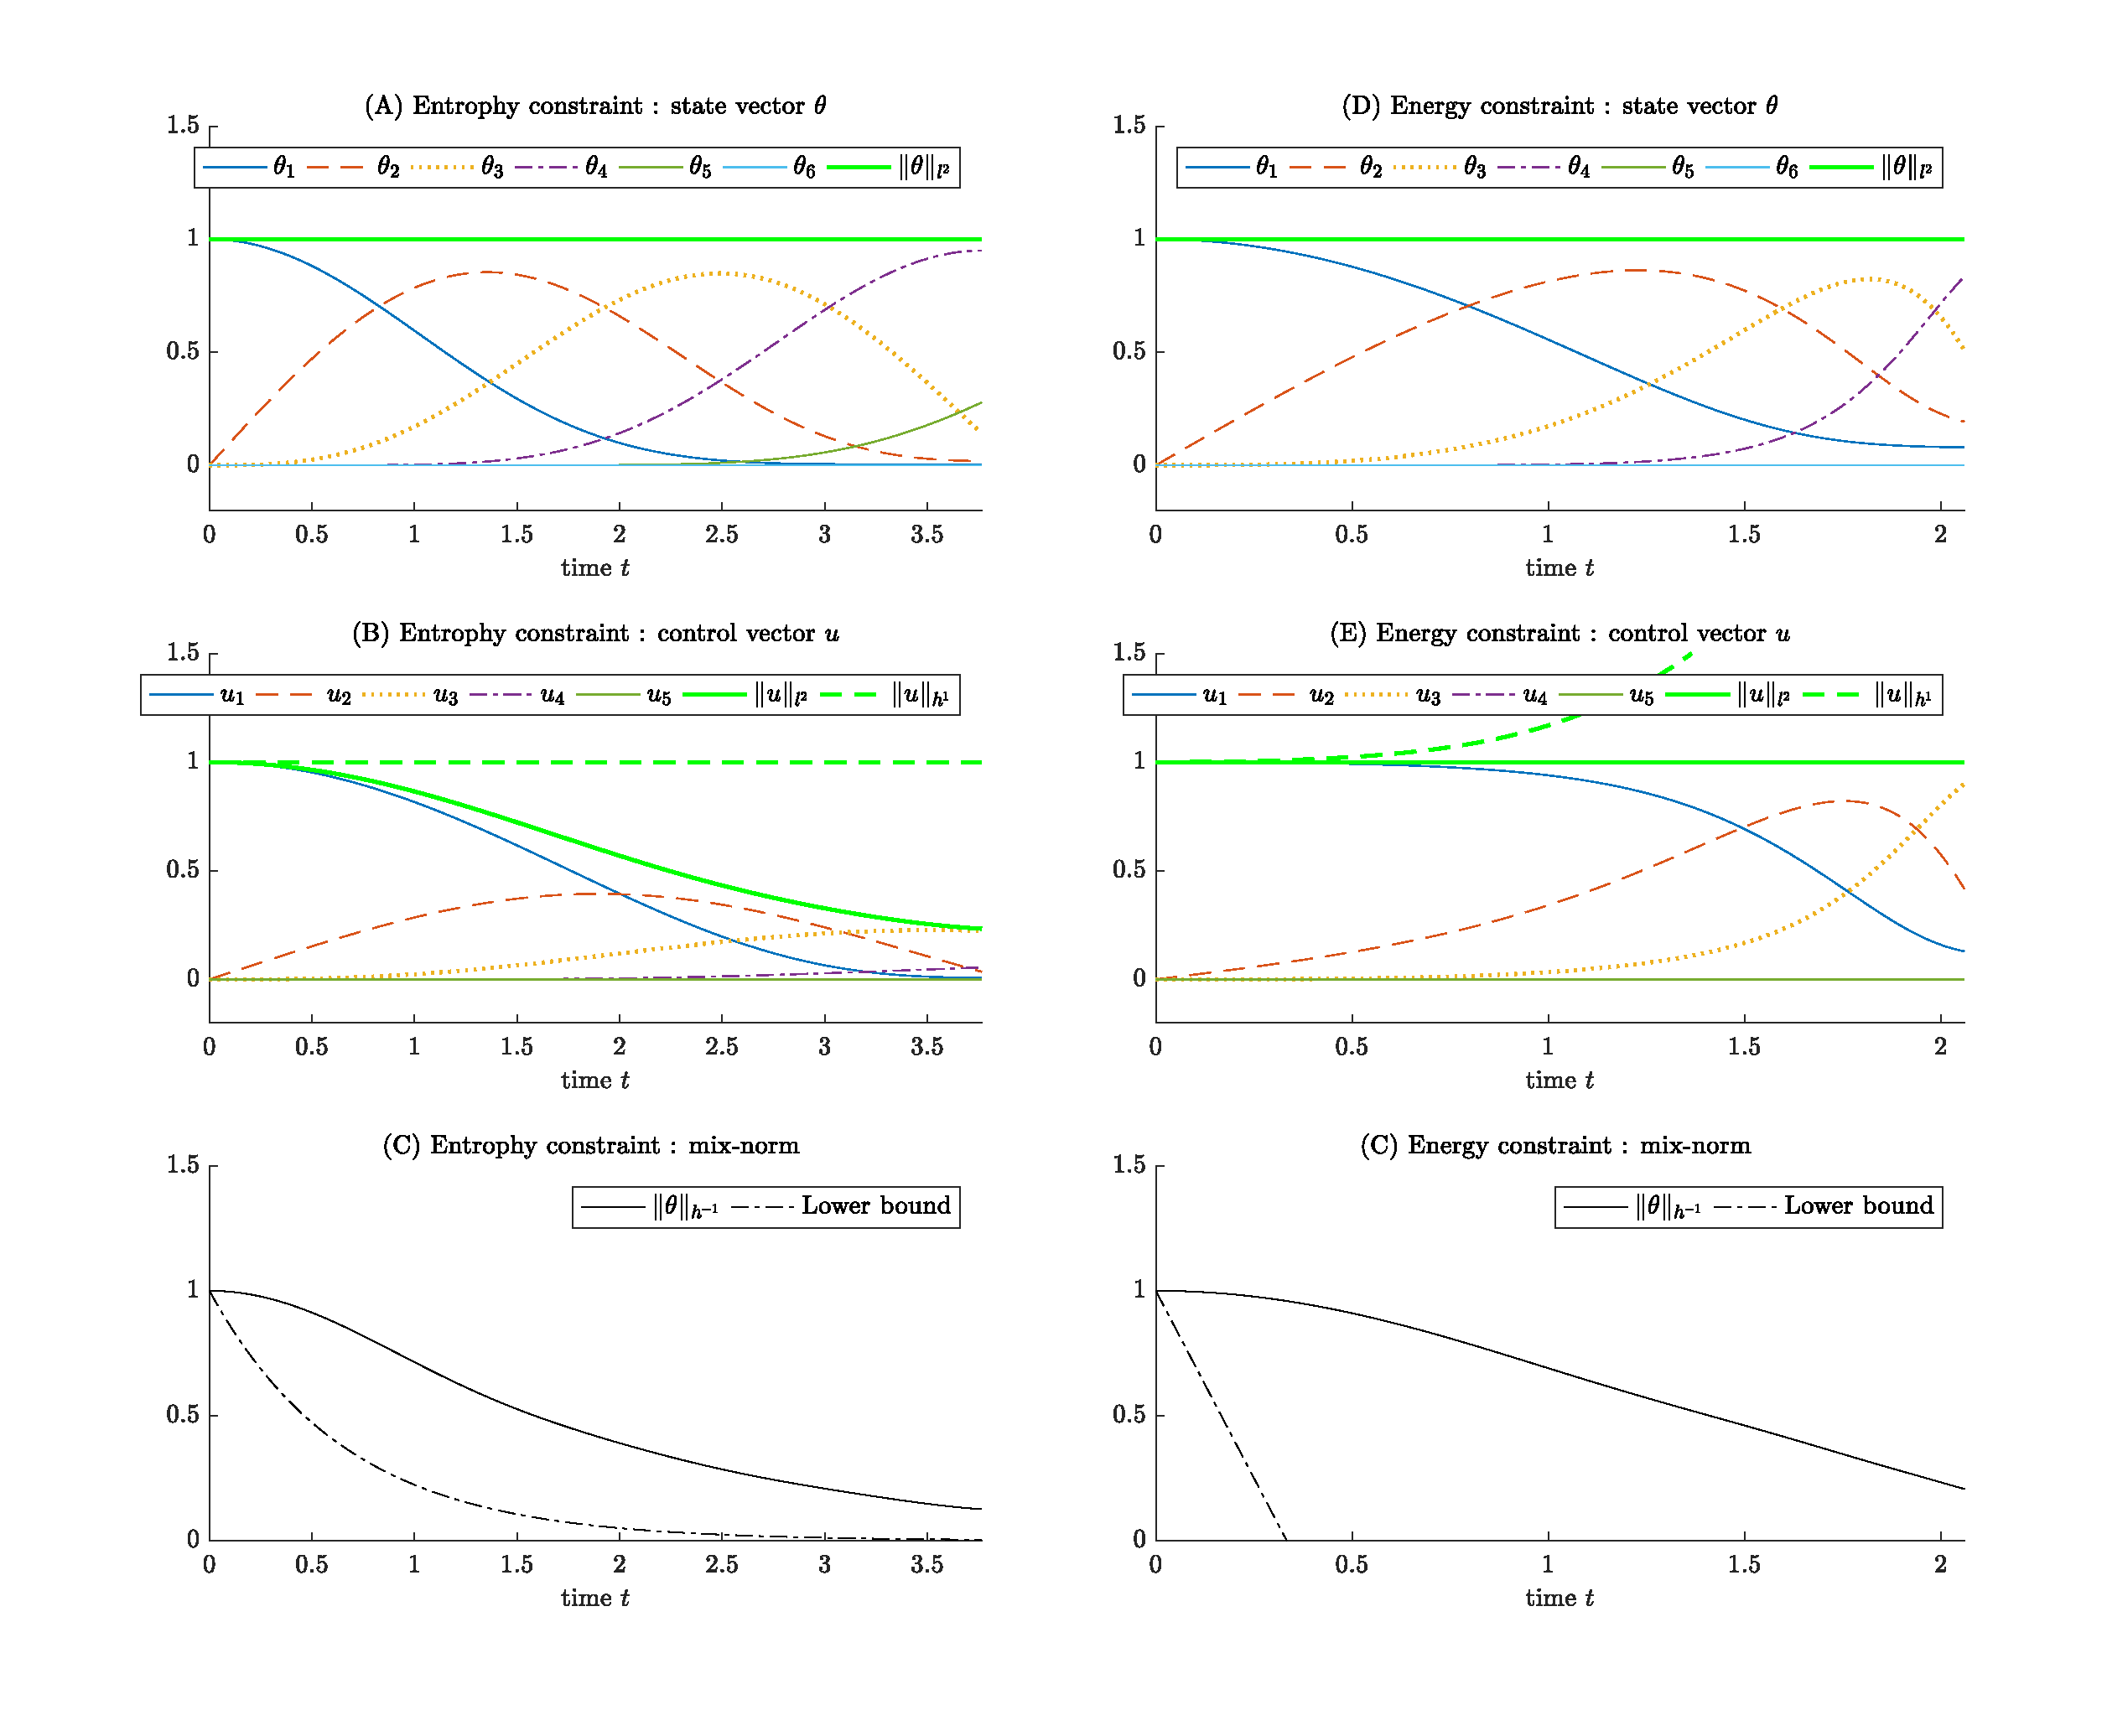
\includegraphics[width=1.0\textwidth]{ch-shellmodel/images/git_muic}
	\caption{Global-in-time strategy applied to the 6-shell truncated model starting initially from the most unmixed state. The entrophy-constrained case ($\frac{1}{\tau}=1, T=3.77 $) is shown on the left subplots where (A) shows the state, (B) shows the control, and (C) shows the mix-norm. The energy-constrained case ($U=1, T= 2.06$) is shown on the right subplots where (D) shows the state, (E) shows the control, and (F) shows the mix-norm.  }
	\label{fig:git_muic}
\end{figure*}



It is uncertain if an analytic solution can be found for arbitrary shell truncation number $N$ and constraint type (enstrophy or energy). However, it is possible to solve the general case numerically by using a gradient-based method (classical gradient descent adapted to converge to a saddle point rather than a minimum).  The algorithm begins with an initial guess for $u(t)=u^{(0)}(t)$ and $\mu=\mu^{(0)}$. Given $u$, we numerically integrate (\ref{eq:first_variation_state}) forward in time to determine $\theta(t)$. We then use the terminal condition $\phi_{n}(T)=\frac{\theta_{n}(T)}{k_{n}^2}$ to provide an `initial' condition for $\phi$ when evolving (\ref{eq:first_variation_adjoint}) backwards in time. We relax the optimality condition (\ref{eq:first_variation_optimality}) and budget constraint (\ref{eq:first_variation_constraint}). Our update rules for $u^{(k)}$ and $\mu^{(k)}$ are given by


\begin{eqnarray}
	\label{eq:update_scheme}
	u^{(k+1)}_{n}&=&u^{(k)}_{n}-\nu_{u} \frac{\delta \mathcal{L}}{\delta u_{n}} \\
	\mu^{(k+1)}&=&\mu^{(k)}+\nu_{\mu} \frac{\delta \mathcal{L}}{\delta \mu_{n}}
\end{eqnarray}
where
\begin{eqnarray}
	\frac{\delta \mathcal{L}}{\delta u_{n}}&=& k_{n}\phi_{n+1}\theta_{n} - k_{n}\phi_{n}\theta_{n+1}+\mu k_{n}^{2\alpha}u_{n} \\
	\frac{\delta \mathcal{L}}{\delta \mu}&=& \frac{1}{T}\int_{0}^{T}\|u\|_{h^{\alpha}} dt - [W^{(\alpha)}]^{2}.
\end{eqnarray}
Our convergence criteria is given by
\[
	\left \| \frac{\delta \mathcal{L}}{\delta u_{n}}\right\|_{l^{\infty}}<\delta  \text{ and }
	\left|\frac{\delta \mathcal{L}}{\delta \mu}\right|<\delta
\]
where both inequalities above must be true to deem convergence with tolerance $\delta$.

Using this method, we computed the optimal solution for the 6-shell truncated model. We choose $\frac{1}{\tau} = 1$ for the enstrophy-constrained case and $U=1$ for the energy-constrained case.  Both cases are shown in figure \ref{fig:git_muic} -- this should be compared with the local-in-time strategy for both constraint types. The rate of mixing with the global-in-time strategy shows improvement over local-in-time strategy in both the enstrophy and energy constrained cases. As first seen in 3-shell truncated model, we again see the `short-cutting' feature where the state vector never visits a $\theta_{n}$ axis as seen in the local-in-time case. Although we only show the case for  $N =6$ as an example, this feature was observed for larger values of $N$. Figure \ref{fig:git_muic} also shows how the mix-norm over time compares to the lower bounds derived in Appendices \ref{appendix:lower_bound_enstorphy_nodiff} and \ref{appendix:bound_energy_no_diff}.



\section{Mixing with diffusion}
\label{sec:diffusivecase}

In this section, we will see how diffusion affects the dynamics. One key characteristic is that the quantity $\|\theta\|_{l^{2}}$ is no longer conserved as shown clearly by the relation (\ref{eq:shell_L2decay}) with positive $\kappa$.

\begin{figure*}[!ht]
	\centering
	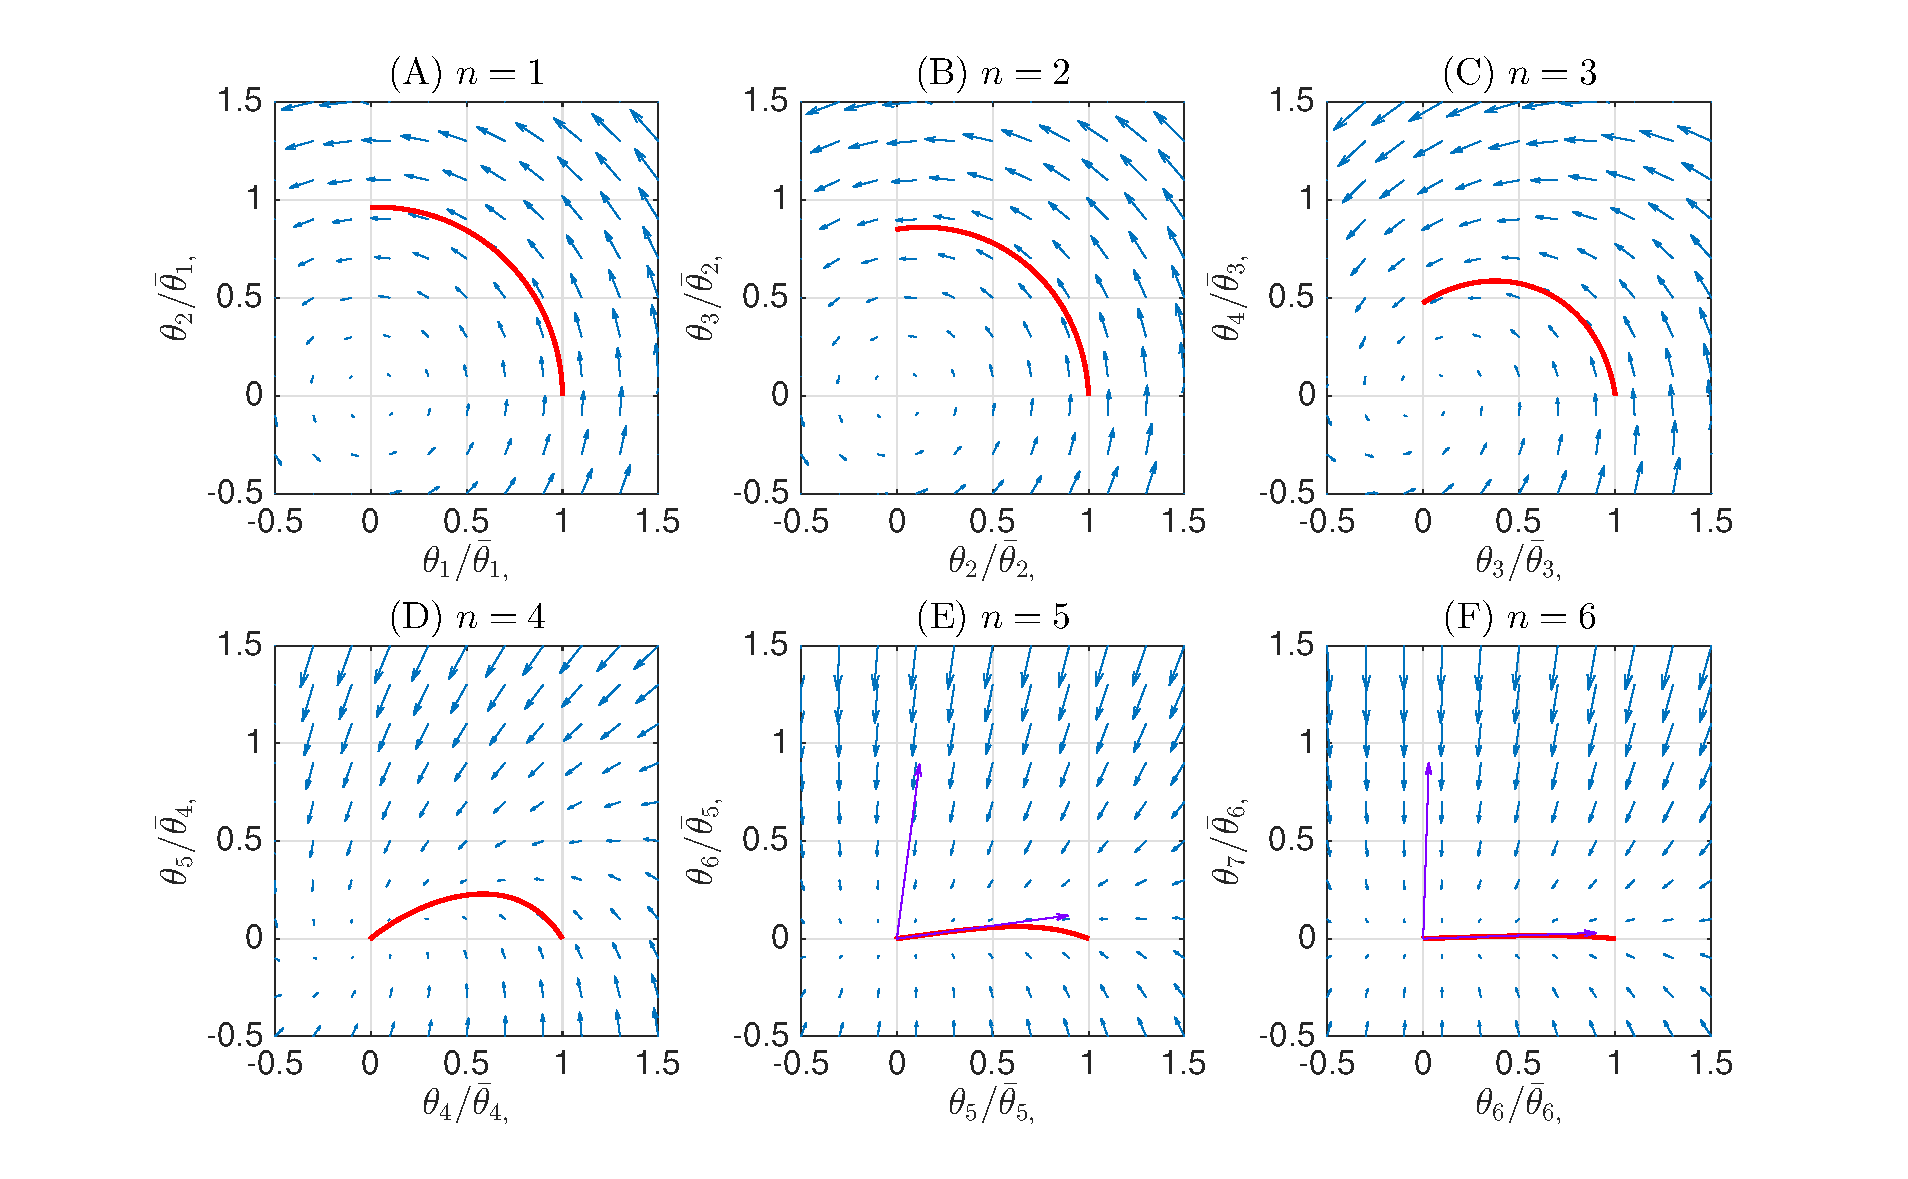
\includegraphics[width=0.8\textwidth]{ch-shellmodel/images/phase_portraits}
	\caption{Local-in-time optimal strategy with diffusion ($\kappa=0.01$) and fixed enstrophy ($1/\tau=1$). The state trajectory is indicated in red and the normalized eigenvectors are purple. The fixed point at the origin is a stable spiral for low values of $n$ and becomes a stable node when $n$ is greater than $4$.  }
	\label{fig:diffusion_phase_portraits}
\end{figure*}



\begin{figure*}[!ht]
	\centering
	\includegraphics[width=1.0\textwidth]{ch-shellmodel/images/lit_diff_muic}
	\caption{Local-in-time strategy with diffusion ($\kappa=0.01$) starting initially from the most unmixed state. The entrophy-constrained case ($\frac{1}{\tau}=1$) is shown on the left subplots where (A) shows the state, (B) shows the control, and (C) shows the mix-norm. The energy-constrained case ($U=1$) is shown on the right subplots where (D) shows the state, (E) shows the control, and (F) shows the mix-norm. Lower bounds from applying {\it Theorem 2} in Appendix \ref{appendix:pmift_impossible} are also shown in subplots (C) and (F).}
	\label{fig:lit_diff_muic}
\end{figure*}

We again consider the same initial condition and local-in-time optimization problem seen in \ref{sec:LIT_MUIC}. Recall that the initial state is the most umixed state, $\theta(0)=(1, 0, 0, \dots )^{T}$. We deal with the generalized constraint (\ref{eq:shellNN_lit_contstraint}) parameterized by $\alpha$. By employing results from the section \ref{sec:LIT}, the optimal strategy is to initially use $u_{1}=W^{(\alpha)}/k_{1}^{\alpha}$ with the other components of $u$ set to zero. Thus,  the motion will initially be in the $\theta_{1}$-$\theta_{2}$ plane with the following reduced state equation

\[
	\frac{d}{dt}\left( \begin{array}{c}
	\theta_{1} \\
	\theta_{2}\end{array} \right)
	=
	\left( \begin{array}{cc}
	-\kappa k_{1}^2 & -k_{1}u_{1} \\
	k_{1}u_{1} & -\kappa k_{2}^2  \end{array} \right)
	\left( \begin{array}{c}
	\theta_{1} \\
	\theta_{2}\end{array} \right).
\]
Once the state encounters the axis $(0,1,0,0, \dots)^{T}$, the optimal strategy will switch to $u_{2}= W^{(\alpha)}/k_{2}^{\alpha}$ until the state encounters the next axis $(0,0,1,0,0 \dots)^{T}$. This trend will continue as long as the state keeps visiting each axis. In general, the motion is governed piecewise in time by the following state equation
\begin{equation}
	\frac{d}{dt}\left( \begin{array}{c}
	\theta_{n} \\
	\theta_{n+1}\end{array} \right)
	=
	\left( \begin{array}{cc}
	-\kappa k_{n}^2 & -k_{n}u_{n} \\
	k_{n}u_{n} & -\kappa k_{n+1}^2  \end{array} \right)
	\left( \begin{array}{c}
	\theta_{n} \\
	\theta_{n+1}\end{array} \right)
\end{equation}
after visiting the $n$th axis where $u_{n}=W^{(\alpha)}/k_{n}^{\alpha}$. The eigenvalue problem can be solved to produce the eigenvalues,

\begin{equation}
\label{eq:eigenvalues_lit}
	\lambda_{\pm}=-\frac{1}{2} \kappa(k_{n+1}^2 + k_n^2) \pm \frac{1}{2}\beta_{n}^{(\alpha)}
\end{equation}
where $\beta_{n}^{(\alpha)}=\sqrt{\kappa^{2}(k_{n+1}^2 - k_n^2)^2 - 4 k_n^{2(1-\alpha)} [W^{(\alpha)}]^2 }$, and eigenvectors, in the $\theta_{n}$-$\theta_{n+1}$ plane,

\begin{equation}
	\Theta_{\pm} = \left(
	\begin{array}{c}
		\frac{1}{2} \kappa(k_{n+1}^2 - k_n^2) \pm \frac{1}{2} \beta_{n}^{(\alpha)}\\
		k_n^{1-\alpha}W^{(\alpha)}
	\end{array}
	\right).
\end{equation}
Define $\Theta_n (t)= (\theta_n(t) , \theta_{n+1}(t) )^{T}$. With the initial condition $\Theta_n (0) = (\bar{\theta}_{n}, 0)$ where $\bar{\theta}_{n}$ is the initial value of $\theta_{n}$ at the $n$th time interval, we obtain the solution
\begin{equation}
	\Theta_{n}(t)= \frac{\bar{\theta}_{n}}{\beta_{n}^{(\alpha)}} \left[e^{\lambda_{+}t}\Theta_{+}- e^{\lambda_{-}t}\Theta_{-} \right].
\end{equation}

The fixed point at the origin is a stable spiral for low values of $n$. However, when
\begin{equation}
\label{eq:critical_n}
	n > n_{c} = \frac{1}{1+\alpha}\log_{2}\left(\frac{2 W^{(\alpha)}}{3 \kappa k _{0}^{1+\alpha}}\right),
\end{equation}
the origin transitions to a stable node. At this point, the trajectory {\it cannot } move to the next plane since it must intercept the $\theta_{n+1}$ axis to do so. Figure \ref{fig:diffusion_phase_portraits} shows how the phase portrait changes with shell number $n$ for the enstrophy-constrained case. Figure \ref{fig:lit_diff_muic} shows the local-in-time strategy for both the fixed enstrophy and energy cases. In other words, it is no longer optimal to keep progressing to the next shell.  This result demonstrates that even the slightest degree of diffusion prohibits the local-in-time strategy from performing perfect mixing in finite time which was possible with the perfectly non-diffusive case ($\kappa=0$).

After seeing how diffusion can drastically change the system behavior under the local-in-time scheme, it is natural to ask ``Is perfect mixing in finite time impossible?'' For the enstrophy-constrained case, we apply {\it Theorem 2} in Appendix \ref{appendix:pmift_impossible} to the initial condition $\theta(0)=(1, 0, 0 , \dots )^{T}$ with $\kappa=0.01$ and $\tau=1$. We find the lower bound on the mix-norm,
\begin{equation}
\hmone{\theta(t)}\geq A\exp(r_{+}t) 
\end{equation}
where $A =   0.0625$ and $r_{+}\approx -2.69249$. For the energy-constrained case with identical parameters and initial condition, we have the lower bound,
\begin{equation}
\hmone{\theta(t)}\geq A\exp(r_{+}t) 
\end{equation}
where $A =   0.007$ and $r_{+}\approx -199.805$. This shows that perfect mixing in finite time is indeed impossible with diffusion.


\begin{figure*}[!ht]
	\centering
	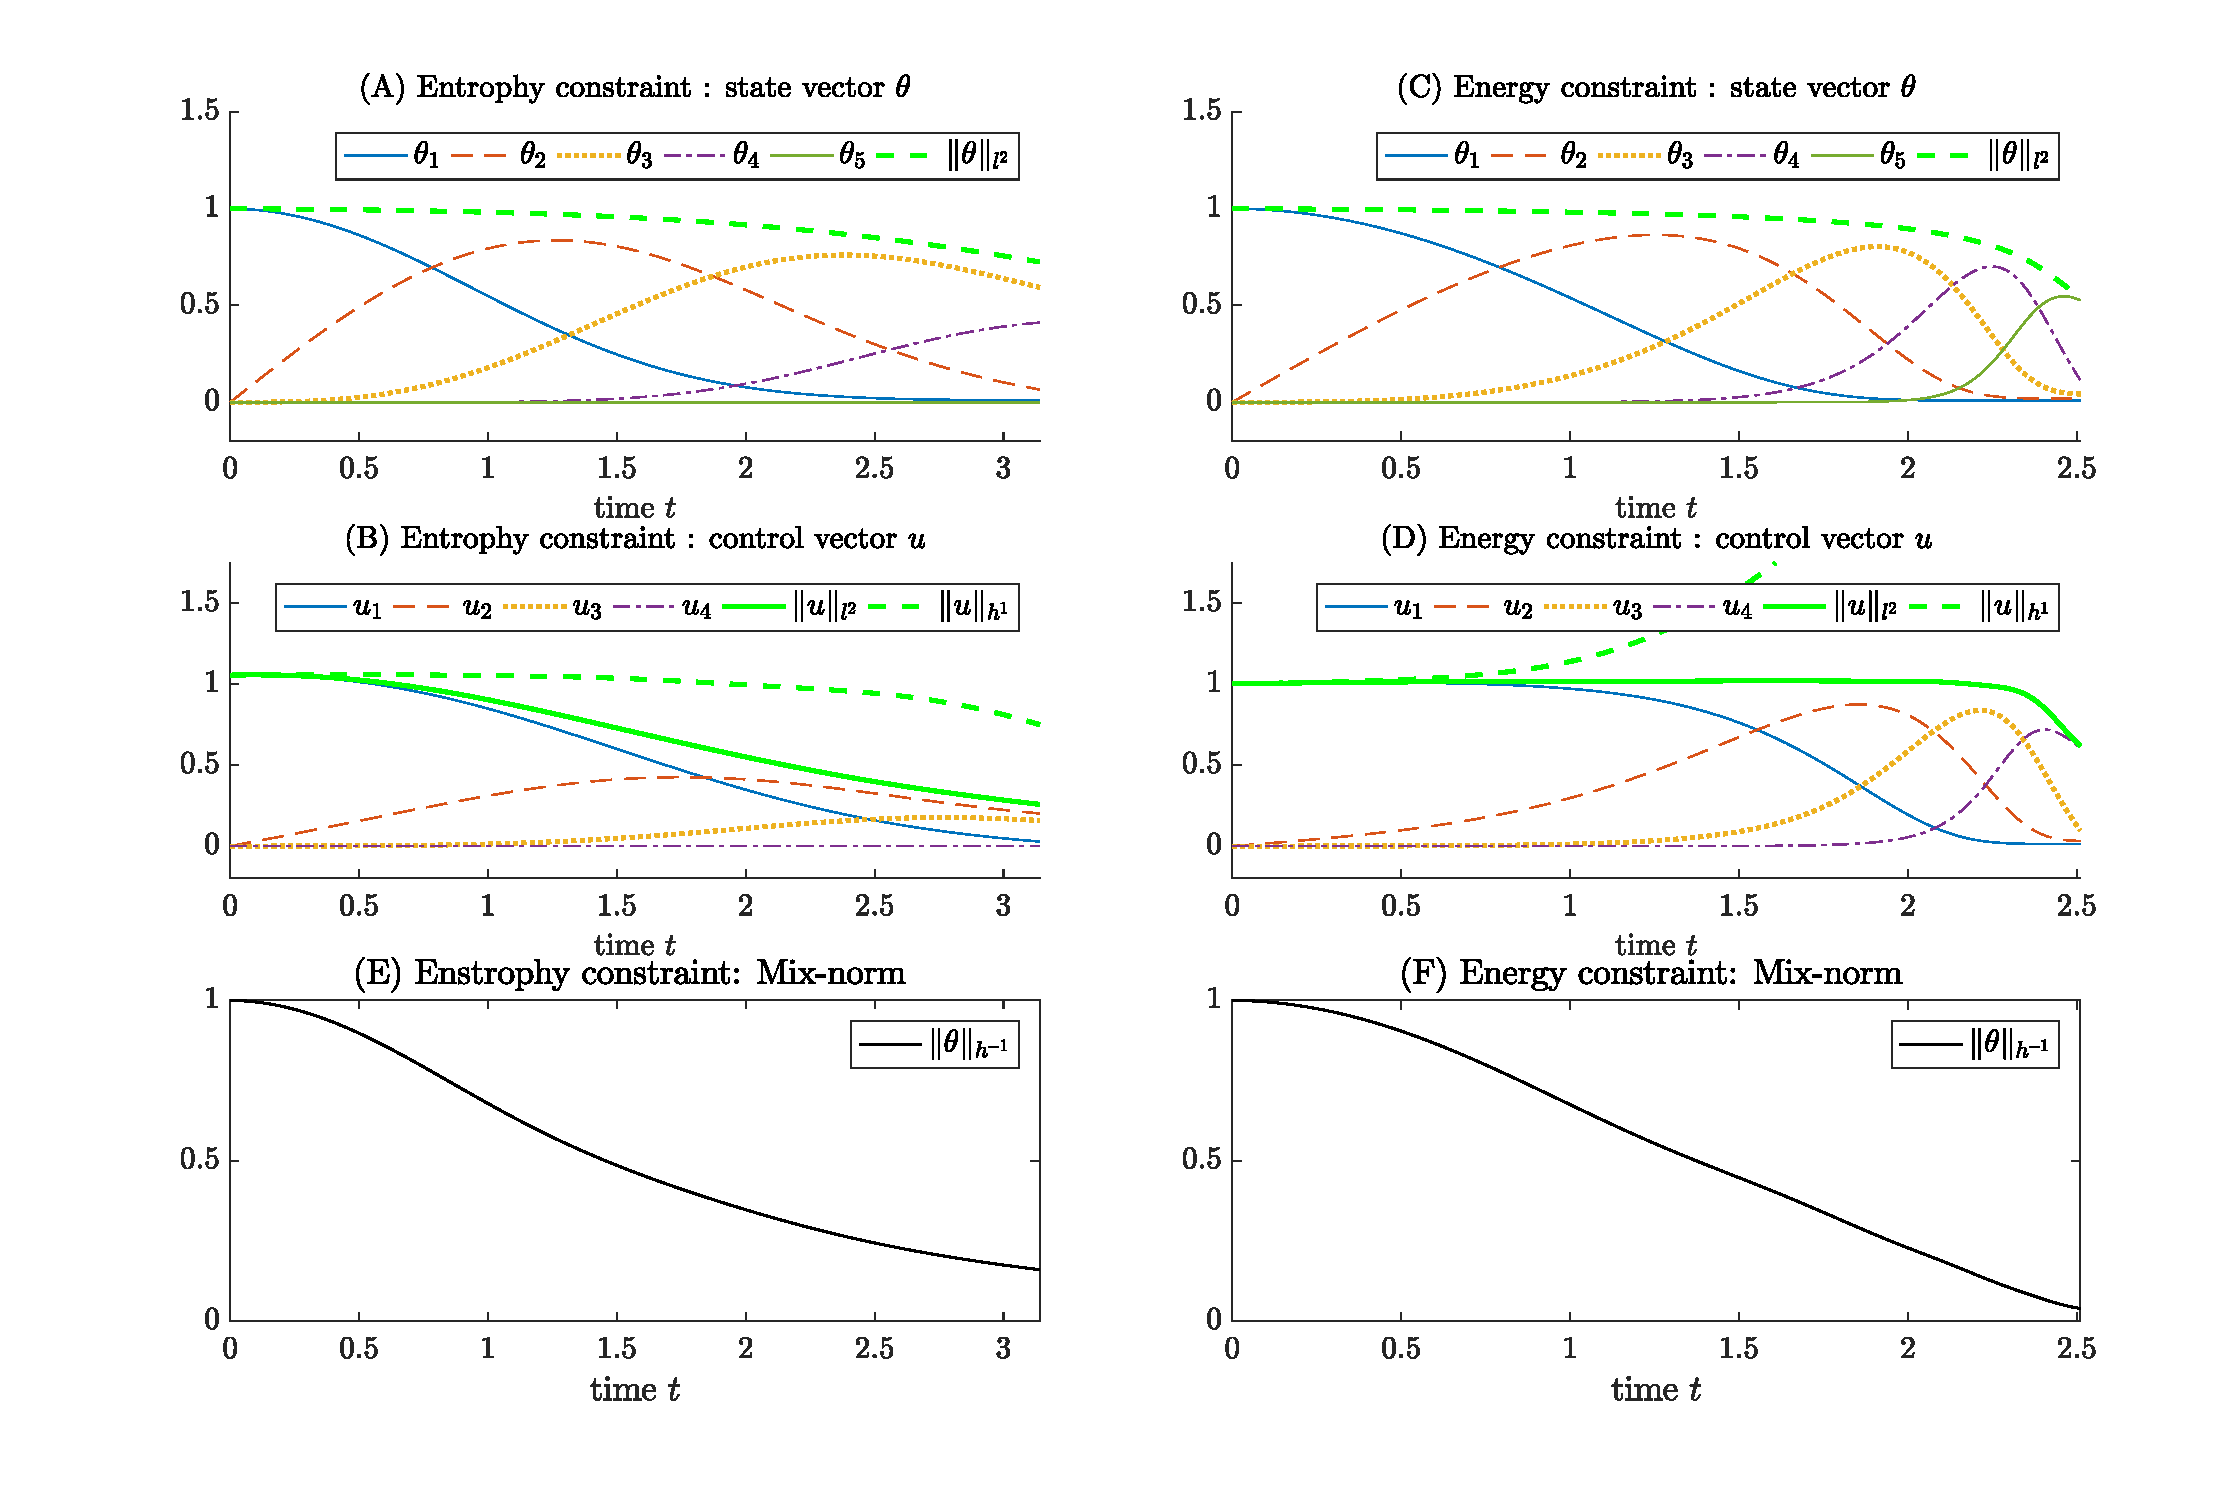
\includegraphics[width=0.9\textwidth]{ch-shellmodel/images/git_diff_muic}
	\caption{Global-in-time strategy applied to truncated shell model ($N=5$) with diffusion ($\kappa=0.01$) starting initially from the most unmixed state. The entrophy-constrained case ($\frac{1}{\tau}=1, T=\pi$) is shown on the left subplots where (A) shows the state, (B) shows the control, and (C) shows the mix-norm. The energy-constrained case ($U=1,T= 0.8\pi$) is shown on the right subplots where (D) shows the state, (E) shows the control, and (F) shows the mix-norm. }
	\label{fig:git_diff_muic}
\end{figure*}


For global-in-time optimization, we use the same numerical scheme detailed in section \ref{sec:ND_GIT_Nshell} here with $\kappa\neq 0$ in equation (\ref{eq:first_variation}). Figure \ref{fig:git_diff_muic} shows the numerical solution for a truncated shell model with $N=5$ and $\kappa=0.01$. The global-in-time strategy appears similar to that with non-diffusive situation in the sense that we see the feature of `short-cutting' relative to local-in-time strategy. We also notice the expected overall decay of the $l^{2}$ norm of $\theta$. We see that the optimal control no longer conserves energy or enstrophy with diffusion. Specifically, we see that it is optimal to use more of the budget earlier on rather than later for both the energy and enstrophy constrained cases.

\section{Discussion}
\label{sec:discussion_shell}
We first focused on mixing without diffusion. The enstrophy-constrained local-in-time strategy exhibited exponential decay while energy-constrained local-in-time strategy showed linear decay --- and hence perfect mixing in finite time. We obtained an analytic solution to the global-in-time optimization problem of the 3-shell truncated model by using methods from nuclear magnetic resonance. The global-in-time strategy applied to the 3-shell truncated model showed an improvement on the mixing rate relative to that of the local-in-time strategy by using a short-cutting method (illustrated in figure \ref{fig:trajectories}). This short-cutting feature generalized to models with higher truncation number $N$. We were surprised to find that it is optimal to use the (energy or enstrophy) budget uniformly in time (rather than consuming more budget earlier than later or vice versa). This is consistent with the work of Mathew {\it et al.} \cite{Mathew2007b} that demonstrated this feature in the partial differential equation context.

Mixing with diffusion was explored and demonstrated interesting effects.  Perfect mixing in finite time for the local-in-time strategy, while constraining either energy or enstrophy, becomes {\it impossible} (recall that it was at least possible for the energy-constrained case without diffusion). The local-in-time dynamics were restricted to $\theta_{n}$-$\theta_{n+1}$ planes piecewise in time similar to that of the local-in-time strategy seen without diffusion. As the state vector progressed to $\theta_{n}$-$\theta_{n+1}$  planes of larger $n$, the diffusive terms progressively dominate over the advective terms in our shell model. Thus, a plane is eventually reached where it is no longer advantageous to progress to the next plane. This suggests that we have succeeded at mixing to a length scale where diffusion can then take over. For energy-constrained flow, this length scale is 
\begin{equation}
\label{eq:batchelor_scale_energy}
l_{u}=\frac{3}{2}\kappa / U.
\end{equation}
For the enstrophy-constrained case, this length scale is  
\begin{equation}
\label{eq:batchelor_scale_enstrophy}
l_{\tau}=\sqrt{\frac{3}{2}\kappa \tau}
\end{equation}
which is naturally interpreted as the Batchelor length scale in turbulent mixing theory \cite{Dimotakis2005,Holzer1994b,Shraiman2000a,Batchelor1959a, Corrsin1951,Obukhov1949}. In fact, (\ref{eq:batchelor_scale_enstrophy}) has the same scaling in molecular diffusivity $\kappa$ and rate-of-strain $1/\tau$ as the turbulent theory type. Local-in-time optimization may suggest that we should mix the tracer concentration until we arrive at these small critical length scales.

But, how should one use a flow intensity budget over time during this approach to small scales? For this, we turn to global-in-time optimization.  Recall that global-in-time optimization without diffusion revealed that it is optimal to use your budget uniformly in time. We find however that this is no longer the case with diffusion. It is optimal to use more of the (energy or enstrophy) budget earlier than later. Therefore, this suggests that budget use is more effective at larger scales away from the Batchelor length scale.

These observations prompt the following questions: ``Will diffusion always dominate advection eventually?'' and ``If so, does this mean that perfect mixing in finite time is impossible?'' We showed in Appendix  \ref{appendix:pmift_impossible} that perfect mixing in finite time is indeed impossible for the enstrophy and energy local-in-time constraints by producing exponential lower bounds on the mix-norm in both cases. 


\begin{figure*}[!ht]
	\centering
	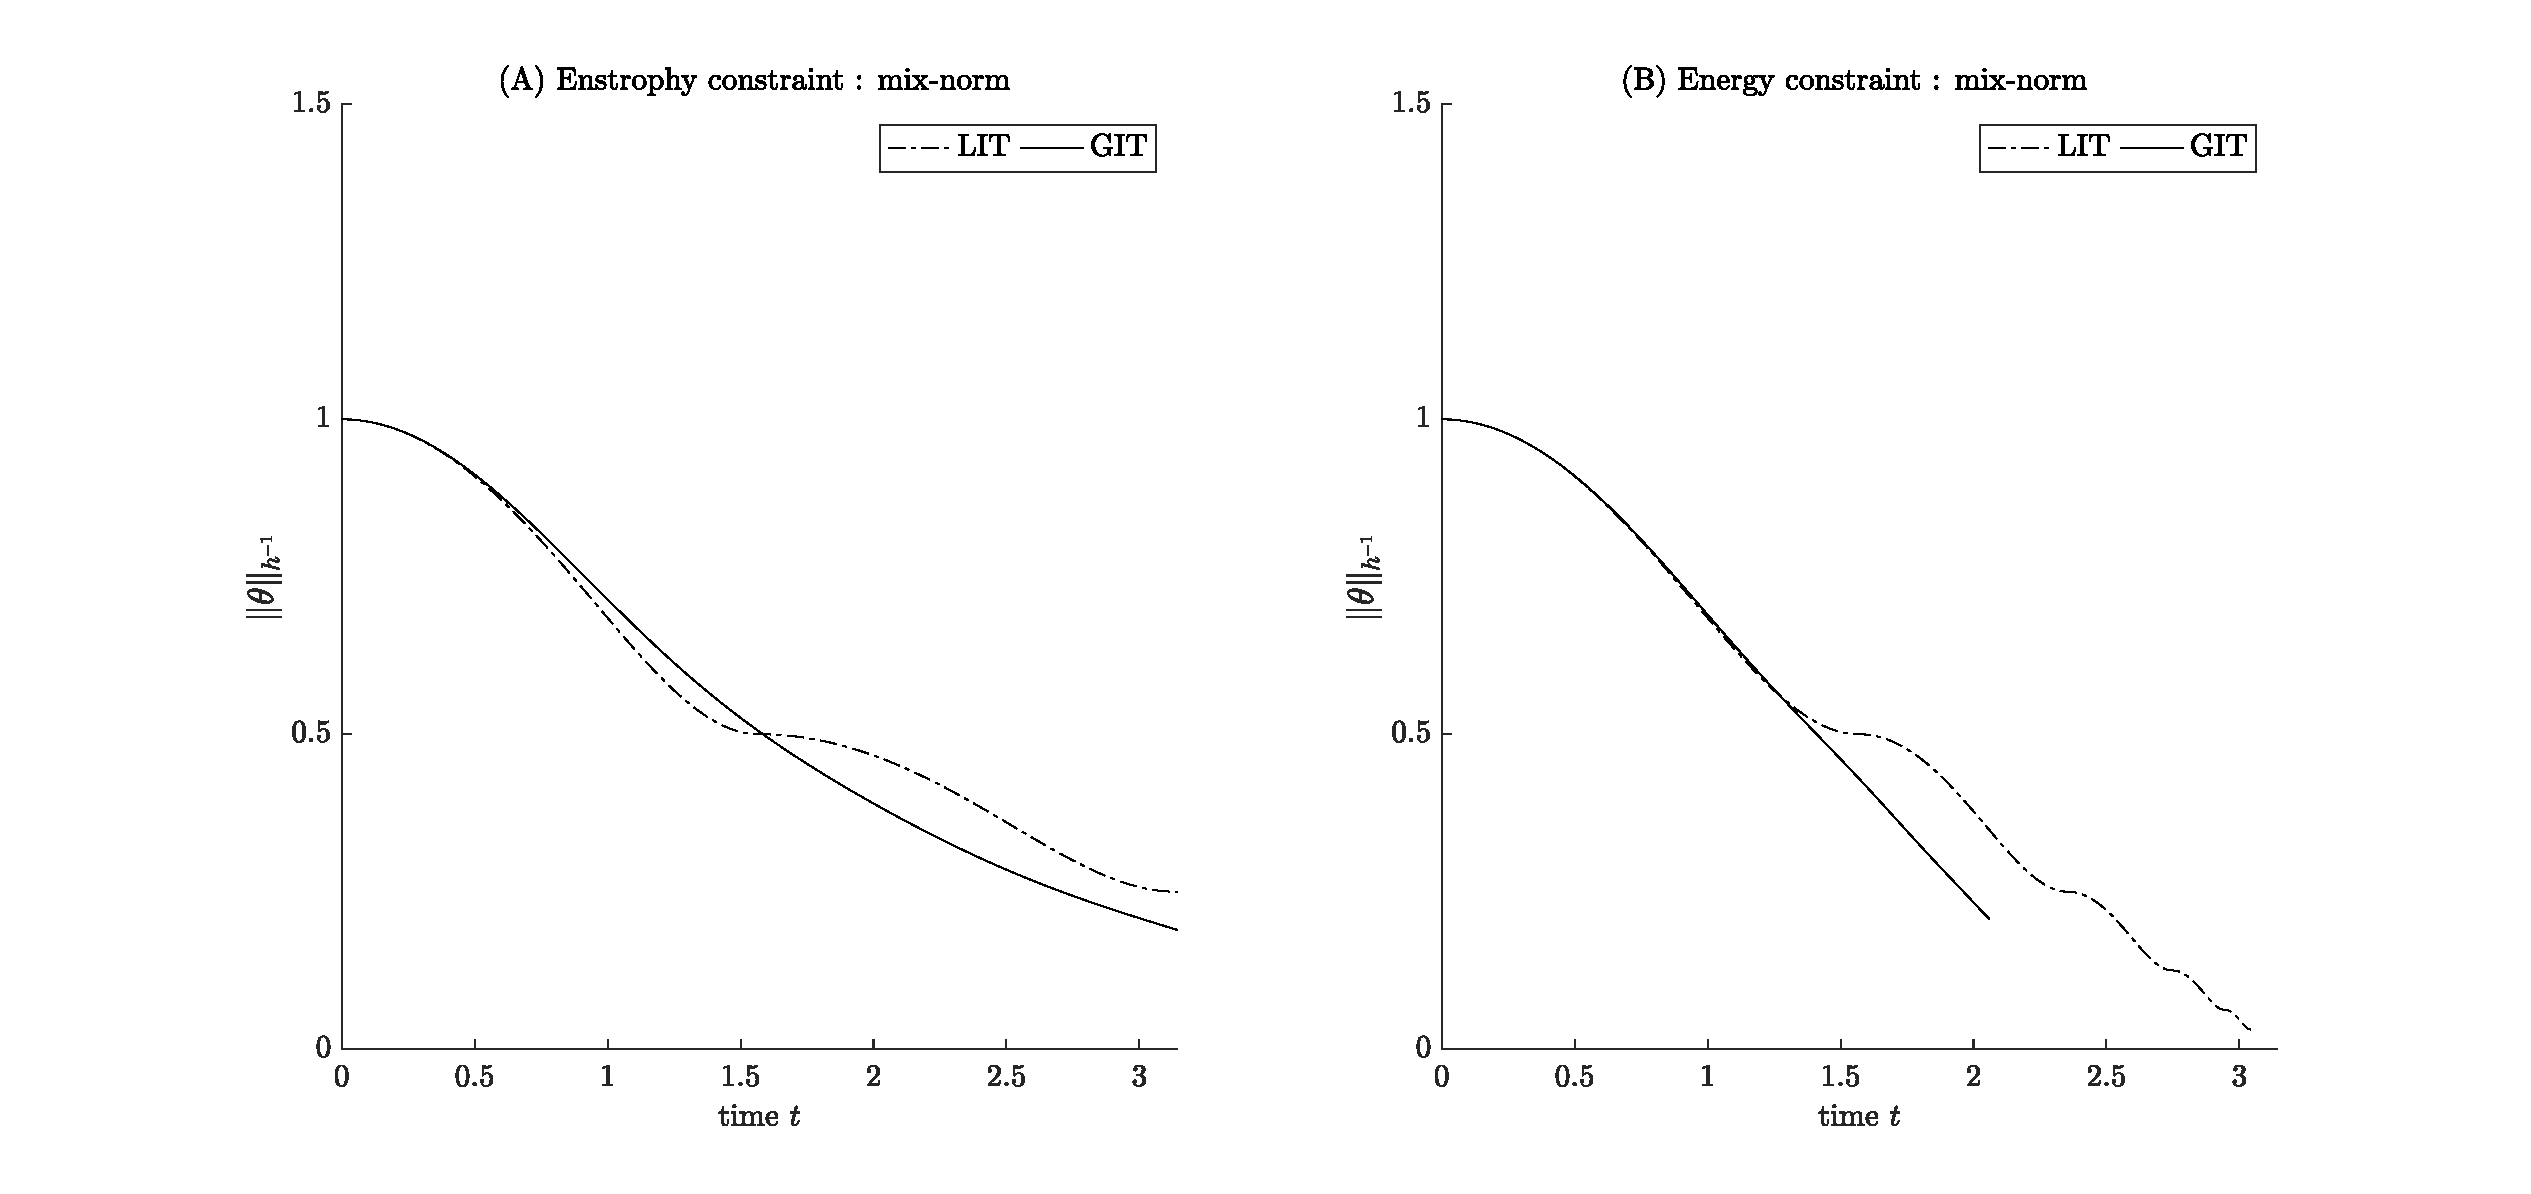
\includegraphics[width=0.8\textwidth]{ch-shellmodel/images/lit_vs_git}
	\caption{The mix-norm over time for the local-in-time (same data from figure \ref{fig:lit_muic}) and global-in-time (same data from figure \ref{fig:git_muic}) strategies applied to the 6-shell truncated shell model without diffusion. The initial condition is $\theta(0)=\mathbf{e}_{1}$. The left plot (A) shows the enstrophy-constrained case with $\tau=1$ and the right plot (B) shows the energy-constrained case with $U=1$. }
	\label{fig:lit_vs_git}
\end{figure*}
\begin{figure*}[!ht]
	\centering
	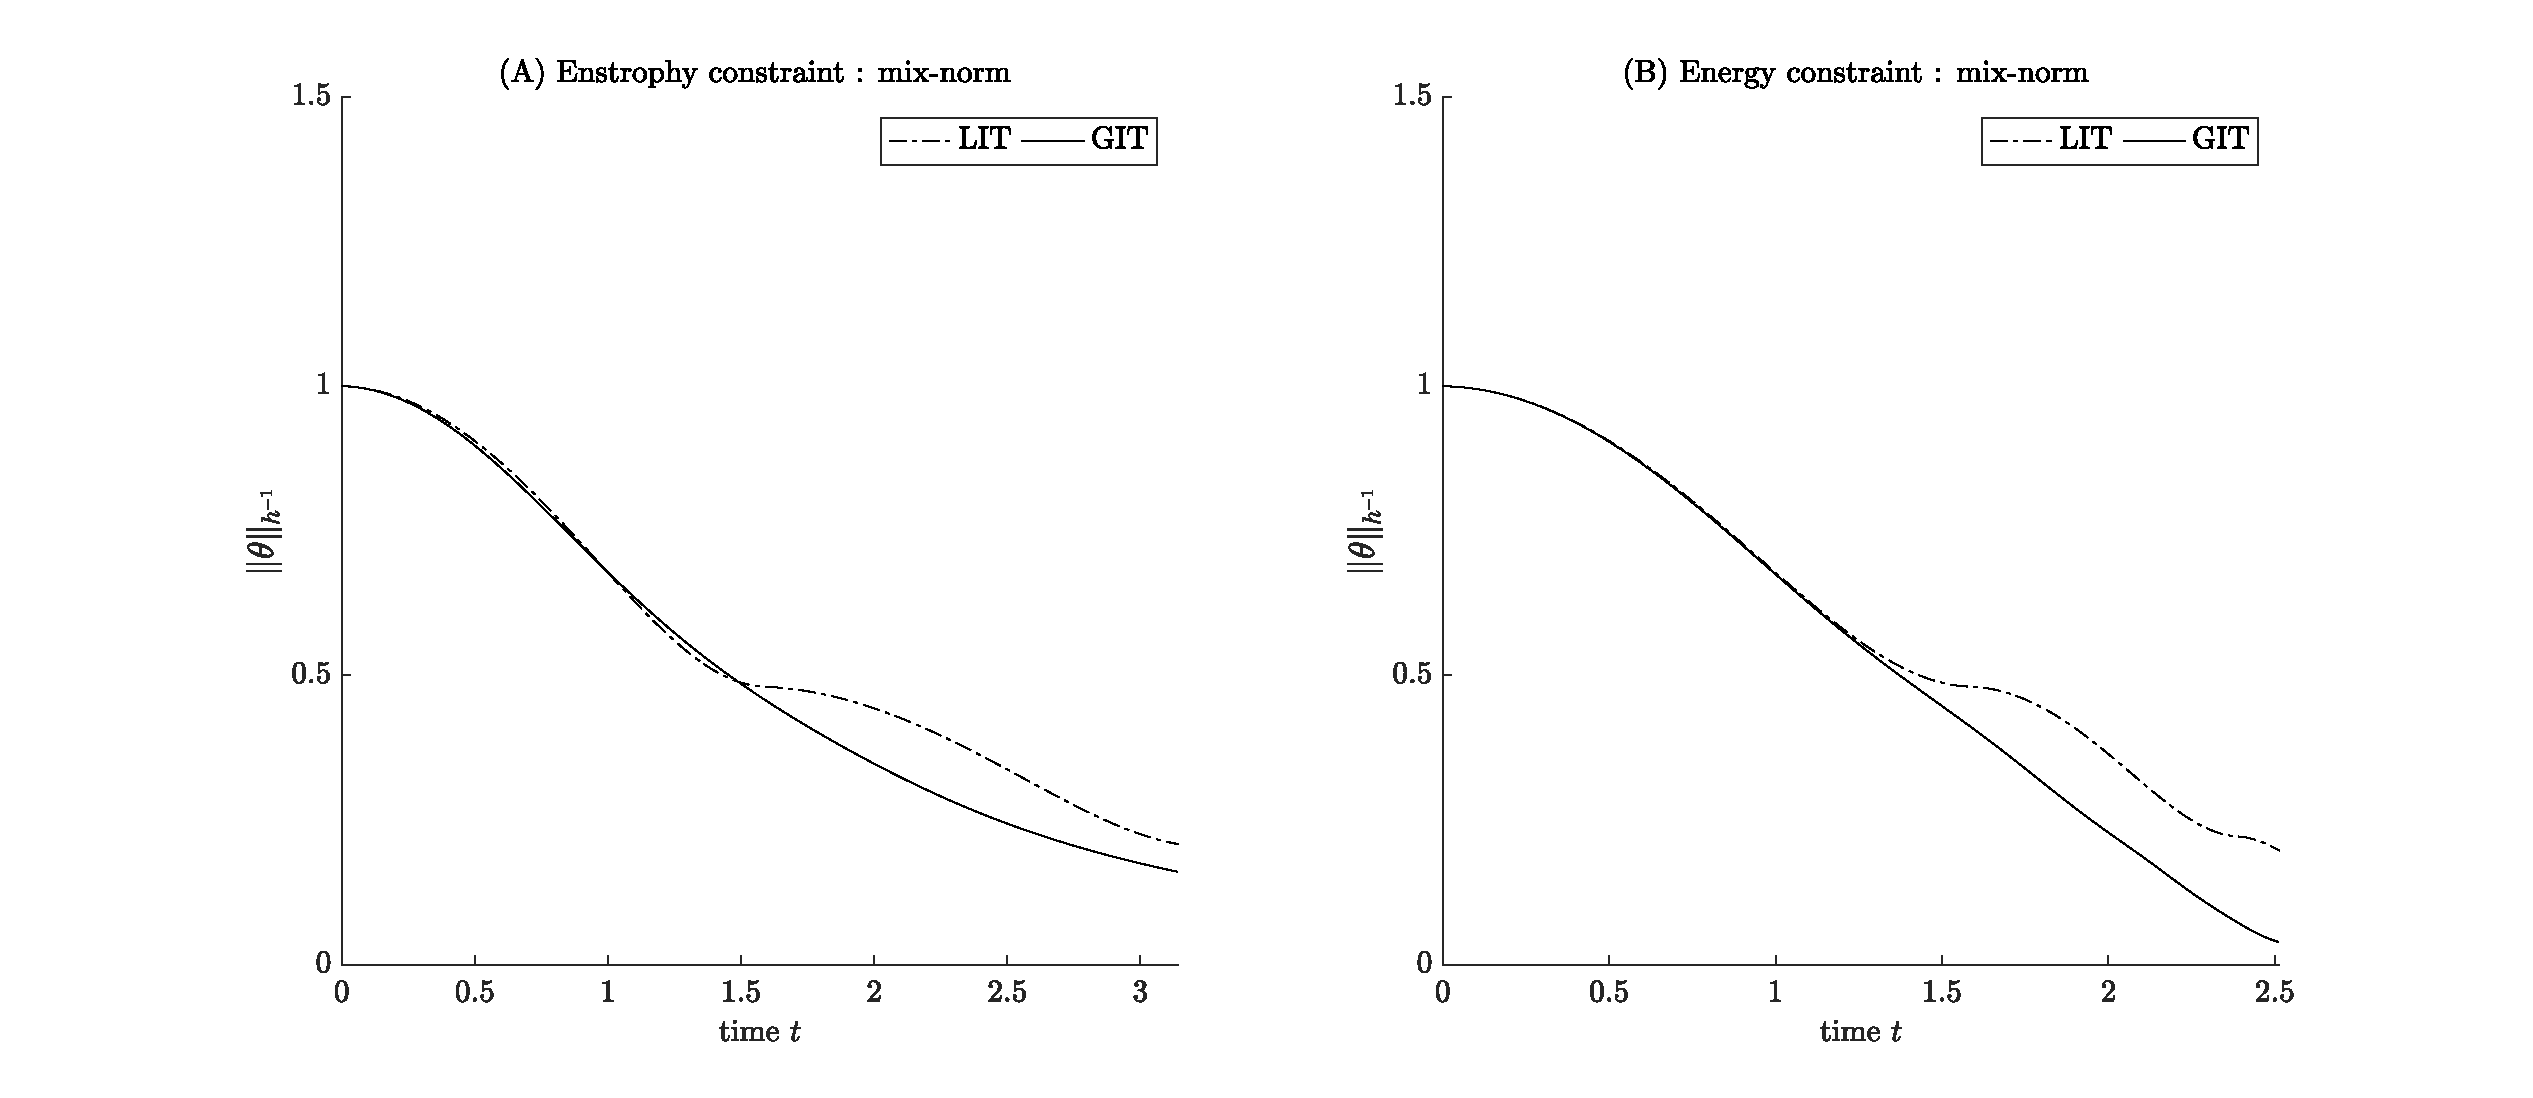
\includegraphics[width=0.9\textwidth]{ch-shellmodel/images/lit_vs_git_diff}
	\caption{The mix-norm over time for the local-in-time (same data from figure \ref{fig:lit_diff_muic}) and global-in-time (same data from figure \ref{fig:git_diff_muic}) strategies applied to the 5-shell truncated shell model with diffusion. The initial condition is $\theta(0)=\mathbf{e}_{1}$. The left plot (A) shows the enstrophy-constrained case with $\tau=1$ and the right plot (B) shows the energy-constrained case with $U=1$. }
	\label{fig:lit_vs_git_diff}
\end{figure*}

 \begin{figure*}[!ht]
	\centering
	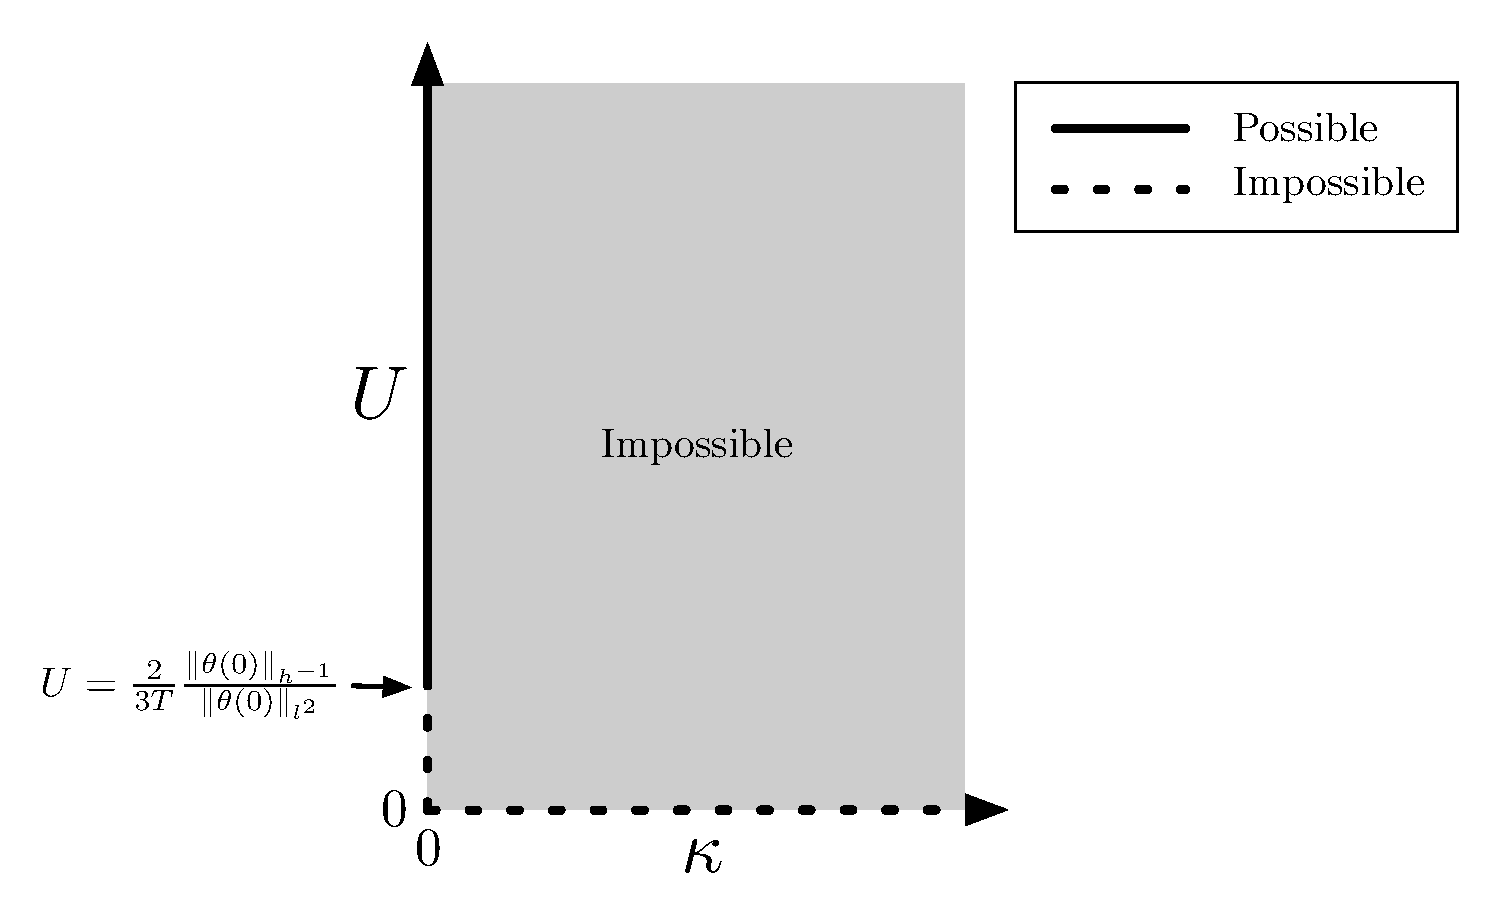
\includegraphics[width=0.5\textwidth]{ch-shellmodel/images/perfectmixing}
	\caption{The possibility of perfect mixing in finite time with energy constraint $\ltwo{u}=U$ and diffusion constant $\kappa$.}
	\label{fig:perfectmixing}
\end{figure*}


In conclusion the developed shell model preserves many known features of the partial differential equation problem. For instance, the shell model performed perfect mixing in finite time without diffusion and with an energy constraint   (Lunasin {\it et al.} \cite{JMP2012}), and showed exponential mix-norm decay without diffusion and with an enstrophy constraint  (Seis \cite{CS2013} and Iyer {\it et al.} \cite{GI2014}).  For the case with diffusion in the partial differential equation setting, it remains to be shown that exponential bounds on the mix-norm exist (as it was shown for the shell model) with $L^{2}$ norm constraints. However for the $L^{\infty}$ extensions of these constraints, strictly positive lower bounds on the mix-norm can be derived by extending the analysis of Poon \cite{Chi-Cheu1996}. This rules out the possibility of perfect mixing in finite time for this situation (and will be discussed further in the next chapter).

Like any reduced model, there are limitations. Some of the bound estimates obtained rely on series inequalities where their integral analogs do not hold  (i.e. for series, we have $\sum_{n} a_{n}b_{n} \leq \sum_{n} a_{n} \sum_{m} b_{m}$ for $a_{n},b_{n}>0$; while for integrals, the analogous expression $\int f(x)g(x) dx$ is not less than $\int  f(x) dx \int  g(x) dx$ for $f,g>0$ in general). Dimensional effects such as incompressibility or integrating volume factors originating in Fourier transforms are neglected. 

Nevertheless, we were able to obtain insights into mixing and arrive at the following answers, in the context of the shell model, to the questions 1 and 2 presented in the introduction:
 \begin{enumerate}
 \item {\it Global-in-time performed slightly better than local-in-time with and without diffusion} (See figures \ref{fig:lit_vs_git} and \ref{fig:lit_vs_git_diff}).

 \item {\it  Without diffusion it is optimal to use a stirring budget uniformly in time; with diffusion it is optimal to expend more of the stirring budget earlier than later.} 
\end{enumerate}
 In fact, it is optimal to use a stirring budget uniformly in time also in partial differential equation context without diffusion (see Chapter \ref{chap:git}). We surmise that the other conclusions hold true in this setting as well.  
 
Furthermore, we found that perfect mixing in finite time is impossible for the enstrophy constraint  $\|u(t)\|_{h^{1}}=\frac{1}{\tau}$ for all values of rate-of-strain $\frac{1}{\tau}\geq 0$ and $\kappa\geq0$. As for the energy-constraint $\|u(t)\|_{l^2}=U$, perfect mixing in finite time is impossible for most of the $U$-$\kappa$ parameter space (see figure \ref{fig:perfectmixing}) except for the singular case of $\kappa=0$ and $U\geq\frac{2}{3T}\frac{\hmone{\theta(0)}}{\ltwo{\theta(0)}}$ that was realized by the local-in-time strategy. Therefore perfect mixing in finite time is a phenomena confined to pure advection ($\kappa = 0$). 





 
 \chapter[Local-in-time optimization]{Local-in-time optimization \footnote{The content of this chapter is included  within a journal article accepted for publication in Nonlinearity \cite{Miles2018}.}}
 \label{chap:lit}
 
\section{Introduction}
\label{sec:introduction}

In this chapter, we make progress towards answering ``What is the most optimal mixing rate in the presence of diffusion for an enstrophy or energy constrained flow?'' This question was also asked in the context of the shell model. We would like to determine if the predictions of the shell model hold in the partial differential equation setting. 

We approach the posed question by considering the general setup, introduced in the introduction chapter, of the evolution of passive scalar in a periodic box. We consider the local-in-time optimization problem introduced by Z. Lin {\it et al.} \cite{JFM2011} in context of pure advection. We now study this optimization problem with the inclusion of diffusion. Local-in-time optimization seeks to find the optimal flow that achieves the best instantaneous mixing rate. We will see that the best choice leads to a $\vec{u}$ that depends on $\theta$. This feedback causes the dynamics of $\theta$ governed by \eqref{eq:PDE_advection} to be nonlinear.

We will demonstrate that homogenization via diffusion and filamentation via advection can sometimes be in conflict and collectively produce a negative impact on mixing. We show numerical evidence that filamentation length scale appears to be limited by the Batchelor scale as seen in the shell model. Even when actively trying to choose the most optimal flow to enhance filamentation. Thus, this may suggest that the Batchelor scale does not only limit turbulent flows but also all incompressible flows under the flow constraints considered here. Although these quantities have been known in the context of turbulence theory, the impact of these limitations on mixing rates has not been fully studied to our knowledge.


The chapter is organized as follows. We introduce the necessary theory regarding local-in-time optimization, a shell model, and $L^{\infty}$ flow constraints in section \ref{sec:theory}. Section \ref{sec:numerical_experiment} details the methodology and results of numerically implementing local-in-time flow optimization. Lastly, we finish with a discussion and conclusion in sections \ref{sec:discussion} and \ref{sec:conclusion} respectively.



%%%
%%%
%%% THEORY
%%%
%%%
\section{Theory}
\label{sec:theory}
\subsection{Local-in-time flow optimization}

We will consider the evolution of a tracer quantity $\theta$ governed by equation \ref{eq:PDE_advection} under an the incompressible flow $\vec{u}$.  Recall the flow is constrained by enstrophy $\ltwo{\nabla\u} = \Gamma L^{d/2}$ or energy $\ltwo{\u} = UL^{d/2}$ where $\Gamma$ is the root mean square rate-of-strain and $U$ is the root mean square speed. 

For the enstrophy-bounded flow problem, we choose the same length scale $L$, the velocity scale $L\Gamma $, and  the time scale $1/\Gamma$. For the energy-bounded flow problem, we non-dimensionalize the system by choosing $L$ as the length scale, $U$ as the velocity scale, and $L/U$ as the time scale.  Both scalings produce the following form of the advection-diffusion equation,
\begin{equation}
\label{eq:nd_ade}
	\ppt{\theta}+\mathbf{u}\cdot \nabla \theta=\frac{1}{Pe} \lap\theta,
\end{equation}
where $Pe=  \frac{\Gamma L^2}{\kappa}$ for the enstrophy-constrained case and $Pe= \frac{UL}{\kappa}$ for the energy-constrained case.   The non-dimensional flow constraints become $\ltwo{\nabla\u} = 1$ or $\ltwo{\u} = 1$.


We consider the local-in-time optimization strategy first introduced by Lin {\it et al.} \cite{JFM2011} in the case without diffusion. We find that this strategy generalizes to the case with diffusion. The local-in-time optimal velocity fields maximize the instantaneous mixing rate by minimizing $\ddt{}\hmone{\theta}^2$. We highlight that local-in-time optimization is not the same as global-in-time or finite-time optimization where the objective is to minimize $\|\theta(\,\cdot\, , T)\|_{H^{-1}}$ at the final time $T$. These objectives generally produce different results.  In the context of the shell model, however, these strategies yielded similar decay rates. The differences between these two objectives under the evolution of  \eqref{eq:nd_ade}  will be the focus of the next chapter and future study. 

The optimal velocity fields are given instantaneously for the enstrophy case by (in non-dimensional form)
%
\begin{equation}
\label{eq:u_lit_enstrophy}
\mathbf{u}= \frac{-\invlap\mathbb{P}(\theta \nabla \invlap\theta)}{\langle |\nabla^{-1}\mathbb{P}(\theta \nabla \invlap\theta)|^2\rangle^{1/2}}
\end{equation}
%
and for the energy case by 
% 
\begin{equation}
\label{eq:u_lit_energy}
\mathbf{u}= \frac{\mathbb{P}(\theta \nabla \invlap\theta)}{\langle |\mathbb{P}(\theta \nabla \invlap\theta)|^2\rangle^{1/2}}
\end{equation} 
%
where $\mathbb{P}$ is the Leray divergence-free projector given by $\mathbb{P}(\vec{v}) = \vec{v} - \nabla \Delta^{-1}(\nabla \cdot \vec{v})$ and $\langle \cdot \rangle$ is the spatial average. These flows will be studied numerically later and is the main focus of this chapter.


We introduce the following measures as useful observables of mixing over time. we use the $H^{-1}$ norm to define the (exponential) rate of mixing as
\begin{equation}
\label{eq:rate}
r(t) = -  \frac{\ddt{}\hmone{\theta}}{\hmone{\theta}}.
\end{equation}
We define the following ratio as a measure of the characteristic filamentation length scale:
\begin{equation}
\lambda(t)\equiv  2\pi \frac{\|\nabla^{-1}\theta(\,\cdot\,,t)\|_{L^{2}}}{\|\theta(\,\cdot\,,t)\|_{L^{2}}}.
\end{equation}
Note that if the tracer concentration field is composed of only one Fourier mode with wave number $\vec{k}$ (i.e. $\theta(\vec{x},t) = Re[ A e^{-i\vec{k}\cdot \vec{x}}]$ where $A$ is a complex constant), then $\lambda(t)$ returns the wavelength of the wave number $\vec{k}$. In general, $\lambda$ is the weighted root mean square wavelength with weights given by $|\theta_{\vec{k}}|^2/\ltwo{\theta}^2$. 


\subsection{Shell model predictions of local-in-time optimization}

The shell model is a model that mimics the spectral dynamics present in the advection-diffusion equation. The model consists of a system of ordinary differential equations with nearest-neighbour coupling between `shells' in wave number space. \cite{Miles2017a} performed local-in-time mixing optimization in this model. The shell-model analysis predicts a limiting length scale given by the Batchelor scale, $\Lambda_{\Gamma} =\sqrt{\frac{\kappa}{\Gamma}}$  and its generalization $\Lambda_{U}= \frac{U}{\kappa} $. The non-dimensional versions are given by $\lambda_{\Gamma}= \frac{1}{\sqrt{Pe}}$ and $\lambda_{U} = \frac{1}{Pe}$. From here forward, we will refer to the Batchelor scale to mean either $\lambda_{\Gamma}$ or its generalization $\lambda_{U}$.  The predicted long-term rates (after reaching the Batchelor scale) are given by $R_{\Gamma} =\kappa/\lambda_{\Gamma}^2 $  and  $R_{U}=\kappa/\lambda_{U}^2$.  The non-dimensional versions are given by $r_{\Gamma} =1$ and $r_{U} = Pe $.

\subsection{Bounds for $L^{\infty}$ constrained flows}
We now consider a subset of $L^{2}$ constrained flows --- those belonging to $L^{\infty}$. In this restricted setting the rate-of-strain and speed are bounded point-wise uniformly in space and time rather than demanding that they merely be $L^2$ integrable as before. Similar analysis of what follows has been attempted in the context of $L^2$ constrained flows, but without success, and appears to be challenging. Thus, we focus on these restricted $L^{\infty}$ constrained subsets of flows where we have been successful at determining bounds on $\lambda$ and measures of mixing. 

\label{sec:linfty_flows}
\subsubsection{Results for $\linf{\nabla \vec{u}} = 1$}

From \eqref{eq:nd_ade}, we find
%
\begin{equation*}
	\frac{1}{(2\pi)^2}\ddt{\lambda^2} = \frac{2}{Pe}
		\left[ 
			\frac{\hone{\theta}^2\hmone{\theta}^2}
					{\ltwo{\theta}^4}  
			- 1
		\right]
		+ 2 \frac{\sint{\nabla^{-1}\theta \cdot \nabla\vec{u} \cdot 
							\nabla^{-1}\theta  }}
					  {\ltwo{\theta}^{2}}
\end{equation*}
and by H\"older's inequality, we deduce
\begin{equation*}
\label{eq:length_ineq_rate-of-strain}
	\frac{1}{(2\pi)^2}\ddt{\lambda^2} \geq \frac{2}{Pe} \left[ 
			\frac{\hone{\theta}^2\hmone{\theta}^2}
					{\ltwo{\theta}^4}  
			- 1
		\right] - \frac{2}{(2\pi)^2}  \lambda^2 .
\end{equation*}
This establishes a lower bound on $\lambda$ at each instant: by apply Gr\"onwall's inequality and the fact that the bracketed term is greater than or equal to zero, it follows that
%
\begin{equation}
\label{eq:exponential_enstrophy}
	\lambda (t) \geq \lambda(0)e^{- t}.
\end{equation}
%


Furthermore,
%
 \begin{eqnarray*}
\frac{d}{dt}\left(\frac{\|\nabla\theta\|_{L^{2}}^2}{\|\theta\|_{L^{2}}^2}\right) &= \frac{\|\theta\|_{L^{2}}^2\frac{d}{dt}\|\nabla\theta\|_{L^{2}}^2-\|\nabla\theta\|_{L^{2}}^2\frac{d}{dt}\|\theta\|_{L^{2}}^2}{\|\theta\|_{L^{2}}^4}\\
&= \frac{-2\sint{\nabla\theta \cdot \nabla\vec{u} \cdot \nabla\theta  } - \frac{2}{Pe} \|\Delta\theta\|_{L^{2}}^2}{\|\theta\|_{L^{2}}^2}+\frac{2}{Pe}\frac{\|\nabla\theta\|_{L^{2}}^4}{\|\theta\|_{L^{2}}^4} \\
&=-\frac{2}{Pe}\left(\frac{\|\Delta\theta\|_{L^{2}}^2}{\|\theta\|_{L^{2}}^2} - \frac{\|\nabla\theta\|_{L^{2}}^4}{\|\theta\|_{L^{2}}^4} \right) - 2\frac{\sint{\nabla\theta \cdot \nabla\vec{u} \cdot \nabla\theta  }}{\|\theta\|_{L^{2}}^2} 
\\
&\leq 2 \frac{\hone{\theta}^2}{\ltwo{\theta}^2}
\end{eqnarray*}
%t
and using $\ddt{}\ltwo{\theta}^2 = -\frac{2}{Pe} \hone{\theta}^2$, it follows that
\begin{equation}
\ltwo{\theta}\geq  \ltwo{\theta_{0}}\exp\left[-\frac{1}{2Pe}\frac{\hone{\theta_{0}}^2}{\ltwo{\theta_{0}}^2}\left(e^{2 t} -1\right)\right].
\end{equation}
Using this with \eqref{eq:exponential_enstrophy}, we deduce the double exponential lower bound
\begin{equation}
\hmone{\theta} \geq  \hmone{\theta_{0}} \exp\left[- t -\frac{1}{2 Pe}\frac{\hone{\theta_{0}}^2}{\ltwo{\theta_{0}}^2}\left(e^{2 t} -1\right)\right].
\end{equation}
Therefore, perfect mixing in finite time is impossible for bounded rate-of-strain flows.

\subsubsection{Results for $\linf{\u}= 1$}
Here we follow and refine an analysis of Poon \cite{Chi-Cheu1996} to show that the presence of diffusion also rules out perfect mixing in finite time for bounded velocity flows as well.  First note that
%
\begin{eqnarray*}
	 \hone{\theta}^2 &=& - 2\sint{\theta \lap \theta} \\
	 							&=& Pe \sint{\theta\left(\ppt{\theta}
	 									-\frac{1}{Pe}\lap \theta\right)} 
	 									-Pe \sint{\theta\left(\ppt{\theta}
	 									+\frac{1}{Pe}\lap \theta\right)},
\end{eqnarray*}
%
\begin{eqnarray*}
	\ddt{}\ltwo{\theta}^2 &=& 2\sint{\theta\ppt{\theta}} \\
										 &=&\sint{\theta\left(\ppt{\theta}
	 									-\frac{1}{Pe}\lap \theta\right)} 
										 + \sint{\theta\left(\ppt{\theta}
	 									+\frac{1}{Pe}\lap \theta\right)} ,
\end{eqnarray*}
%
and
%
\begin{eqnarray*}
	\ddt{}\hone{\theta}^2 &=& -2\sint{\ppt{\theta}\lap \theta} \\
	 									&=& Pe \sint{\left(\ppt{\theta}
	 									-\frac{1}{Pe}\lap \theta\right)^2} 
	 									-Pe \sint{\left(\ppt{\theta}
	 									+\frac{1}{Pe}\lap \theta\right)^2} .
\end{eqnarray*}
%
Then simplify and compute:
%
\begin{eqnarray*}
	\ddt{} \pbrac{ \frac{\hone{\theta}^2}{\ltwo{\theta}^2} } 
			&=& \frac{1}{\ltwo{\theta}^4}
			\sbrac{
				\ltwo{\theta}^2\ddt{}\hone{\theta}^2
				-\ddt{}\ltwo{\theta}^2\hone{\theta}^2			
			}\\
			&=& \frac{1}{\ltwo{\theta}^2}
			 \Bigg[ Pe \sint{\left(\ppt{\theta} -\frac{1}{Pe}\lap \theta\right)^2}  \\
 				& & \qquad\qquad\qquad \qquad \qquad 
				-Pe\sint{\left(\ppt{\theta}+\frac{1}{Pe}\lap \theta\right)^2} 
			\Bigg]\\
		        &-&\frac{1}{\ltwo{\theta}^4}
			\Bigg[ 
				Pe \pbrac{\sint{\theta\left(\ppt{\theta}-\frac{1}{Pe}\lap \theta\right)} }^2\\
 				& & \qquad\qquad\qquad \qquad
				-Pe\pbrac{
					 \sint{\theta\left(\ppt{\theta}
	 									+\frac{1}{Pe}\lap \theta\right)} 
 				}^2					
			\Bigg].
\end{eqnarray*}
%
Using H\"older's inequality and \eqref{eq:nd_ade}, this simplifies to the observation originally noted by Poon \cite{Chi-Cheu1996}:
%
\begin{eqnarray}
	\ddt{} \pbrac{ \frac{\hone{\theta}^2}{\ltwo{\theta}^2} } 
			&\leq & \frac{Pe}{\ltwo{\theta}^2}
			\sbrac{
					 \sint{(\vec{u}\cdot \nabla \theta)^2} 
			}.
\end{eqnarray}
Now applying H\"older's inequality again we have
\begin{equation}
\label{eq:k2growth_energy}
	\ddt{} 
		\pbrac{ 
			\frac{\hone{\theta}^2}{\ltwo{\theta}^2} 
		} 
		\leq  
		Pe
		\frac{\hone{\theta}^2}{\ltwo{\theta}^2} 
\end{equation}
%
and thus 
%
\begin{equation*}
		\frac{\hone{\theta}}{\ltwo{\theta}} 
		\leq  
		\frac{\hone{\theta_0}}{\ltwo{\theta_0}}
		\exp{\pbrac{\frac{Pe}{2} t}}.
\end{equation*}
%
The inequality $\hone{\theta}\hmone{\theta}\geq \ltwo{\theta}^2$ then ensures that
%
\begin{equation}
\label{eq:lambda_bound}
\lambda(t) \geq  2\pi\frac{\ltwo{\theta_0}}{\hone{\theta_0}}\exp{\pbrac{-\frac{Pe}{2}t}}.
\end{equation}
%
Using \eqref{eq:k2growth_energy} together with  $\ddt{}\ltwo{\theta}^2 = -\frac{2}{Pe} \hone{\theta}^2$ we observe that
%
\begin{equation*}
\ltwo{\theta}\geq \ltwo{\theta_{0}}\exp\left[-\frac{1}{Pe^2}\frac{\hone{\theta_0}^2}{\ltwo{\theta_0}^2}\left(e^{Pe \, \, t}-1\right)\right]
\end{equation*}
%
and this combined with  \eqref{eq:lambda_bound} implies another (distinct) double exponential
%
\begin{equation}
\hmone{\theta}\geq \frac{\ltwo{\theta_{0}}^2}{\hone{\theta_0}}\exp\left[-\frac{Pe}{2} \,\, t-\frac{1}{Pe^2}\frac{\hone{\theta_0}^2}{\ltwo{\theta_0}^2}\left(e^{Pe \,\, t}-1\right)\right].
\end{equation}


\section{Numerical experiment: local-in-time optimization}
\label{sec:numerical_experiment}
\subsection{Methodology}


We solve \eqref{eq:nd_ade} with either flow \eqref{eq:u_lit_enstrophy} or \eqref{eq:u_lit_energy} by using a Fourier basis to represent the discretized spatial domain with a 4th order Runge-Kutta time-stepping method.  We slightly perturb the concentration field $\theta_{0}(\mathbf{x}) = \sin(2\pi x/L)$ by evolving the field according to (3) with a steady sin flow given by $\mathbf{u}(\mathbf{x})= \sin(2\pi y/L) \hat{x}$ for a time duration of $0.01$. The concentration field, resulting from this short time integration, is then used as an initial condition for the local-in-time optimization scheme. This perturbation is necessary since the denominator is zero in both expressions (4) and (5) for pure Fourier modes such as $\theta_0$ [2]. The number of Fourier modes is chosen large enough to resolve the spatial resolution and give by the following criteria $N = \min\left[ 2^{ceil(log_2(4(M-1) + 6))} , 512 \right]$ where $M = L/(0.25 \lambda_{B})$ and $\lambda_{B}$ is the appropriate Batchelor scale; The choice of $N = 2^{ceil(log_2(4(M-1) + 6))}$ is suggested as a rule-of-thumb by Ref. \cite{Boyd2000}. The cap of $512$ is suitable for the range of Pe values considered --- the Batchelor wavenumber $k_{B} = 2\pi/\lambda_{B}$ is well within the range of Fourier modes present even after considering $2/3$ dealiasing. The time step is chosen by the CFL condition $dt = 0.25\min\left[L/(UN) , L^2/(\kappa N^2)\right]$ for the enstrophy-constrained case and $dt = 0.25\min\left[1/(\Gamma N) , L^2/(\kappa N^2)\right]$ for the energy-constrained case. All simulation code was created in the programming language Python with package modules, pyfftw and numpy. The code is provided in Appendix \ref{app:lit}.


%%%
%%%
%%% RESULTS
%%%
%%%


\subsection{Results}

\begin{figure}
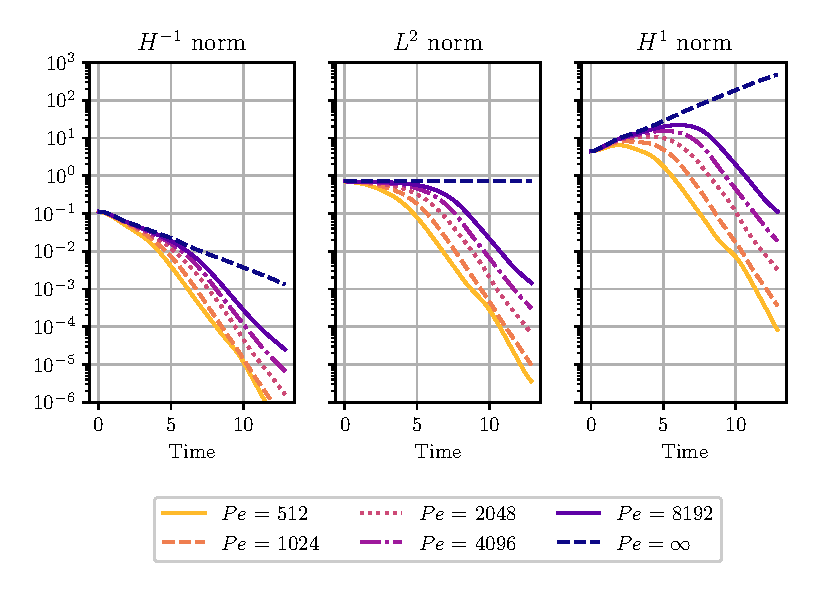
\includegraphics[width=\textwidth]{ch-lit/images/enstrophy_norms}
\caption{$H^{-1}, L^{2},$ and $H^{1}$ norms of the concentration field under the optimal enstrophy-constrained flow.  }
\label{fig:enstrophy_norms}
\end{figure}
%
\begin{figure}
\centering
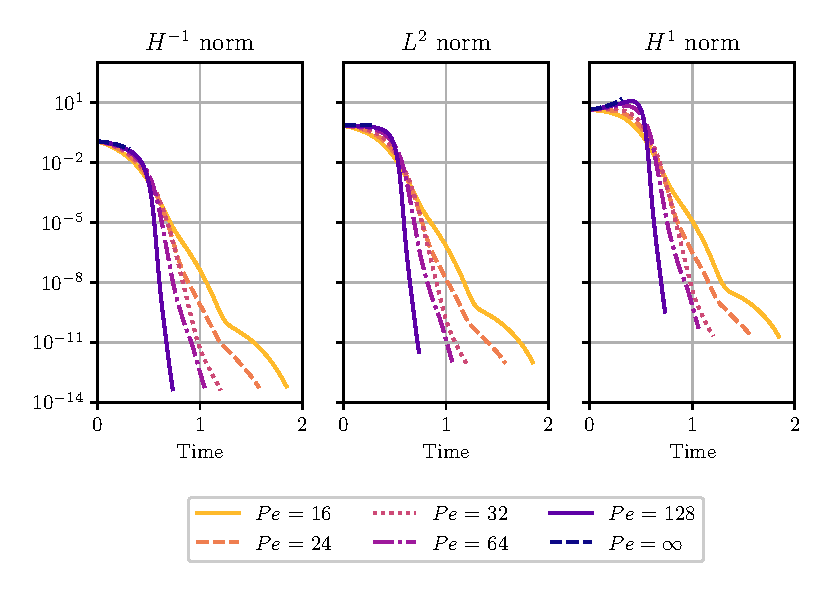
\includegraphics[]{ch-lit/images/energy_norms}
\caption{$H^{-1}, L^{2},$ and $H^{1}$ norms of the concentration field under the optimal energy-constrained flow.}
\label{fig:energy_norms}
\end{figure}


We now investigate the mixing performance under the local-in-time optimal flows. Figure \ref{fig:enstrophy_norms} and \ref{fig:energy_norms} show how the different mixing measures ($H^{-1}$, $L^2$, and $H^{1}$ norms) vary in time for different values of $Pe$ for the enstrophy and energy constrained cases respectively. Notice how the long-term mixing rate appears to be exponential for all three mixing measures. This exponential rate is consistent with shell model predictions, yet weaker than the double-exponential decay rate derived by the $L^{\infty}$ constrained flow analysis.

\begin{figure}
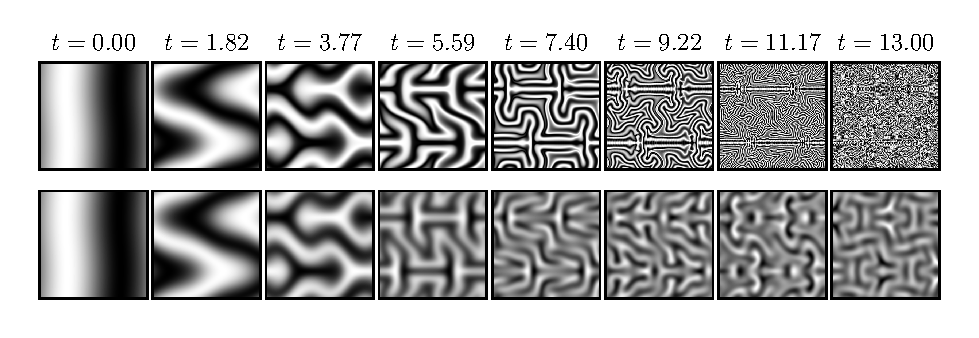
\includegraphics[]{ch-lit/images/enstrophy_film}
\caption{Local-in-time optimization with enstrophy constraint. Top filmstrip is for $Pe =\infty$ and the bottom filmstrip is $Pe=2048$. Note that the grey-scale for the $Pe=\infty$ is constant in time while it is adjusted to show the tracer concentration structure in the finite $Pe$ case. }
\label{fig:enstrophy_film}
\end{figure}
%
\begin{figure}
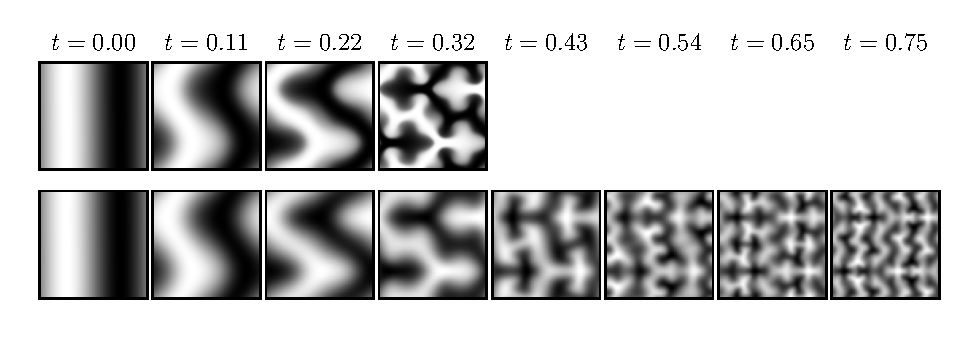
\includegraphics[]{ch-lit/images/energy_film}
\caption{Local-in-time optimization with energy constraint. Top filmstrip is for $Pe = \infty$ and the bottom filmstrip is $Pe=32$. Note that the grey-scale for the $Pe=\infty$ is constant in time while it is adjusted to show the tracer concentration structure in the finite $Pe$ case. The numerical computation is truncated at time $t=0.34$ due to length scales rapidly decreasing past the grid size resolution immediately after $t=0.34$. Fixed energy constrained flows that produce infinitesimally small lengths in finite time have been constructed \cite{JMP2012}. We suspect that the same phenomena may be occurring here.}
\label{fig:energy_film}
\end{figure}
%
\begin{figure}
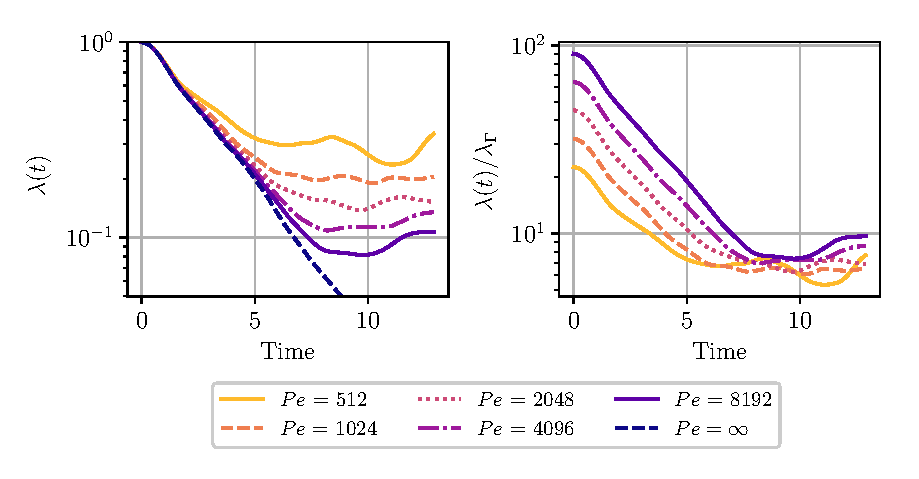
\includegraphics[]{ch-lit/images/enstrophy_length}
\caption{The left subplot shows the filament length $\lambda$ over time subject to the optimal enstrophy-constrained flow. The right subplot is the same data except scaled: $\lambda(t)/\lambda_{\Gamma} = \lambda(t)\sqrt{Pe}$.}
\label{fig:enstrophy_length}
\end{figure}
%
\begin{figure}
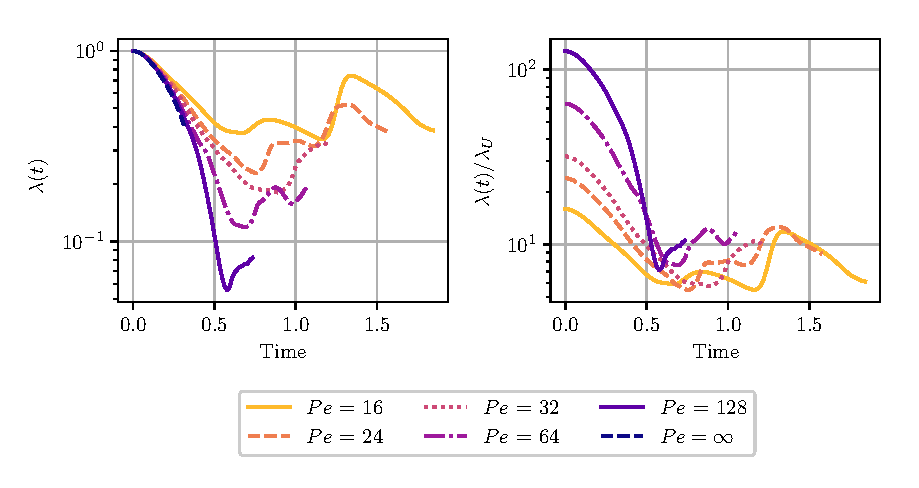
\includegraphics[]{ch-lit/images/energy_length}
\caption{The left subplot shows the filament length $\lambda$ over time subject to the optimal energy-constrained flow. The right subplot is the same data except scaled: $\lambda(t)/\lambda_{U} = \lambda(t) Pe$.}
\label{fig:energy_length}
\end{figure}
%
\begin{figure}
\centering
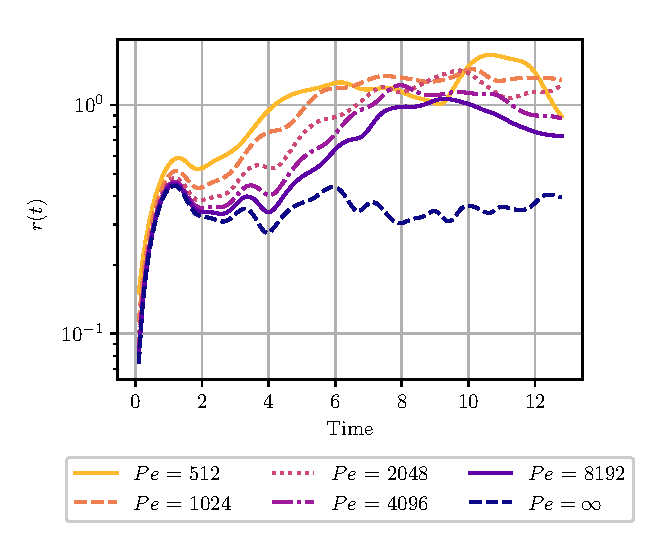
\includegraphics[]{ch-lit/images/enstrophy_rate}
\caption{Mixing rate $r(t)$ over time when subject to the optimal enstrophy-constrained flow.}
\label{fig:enstrophy_rate}
\end{figure}
%
\begin{figure}
\centering
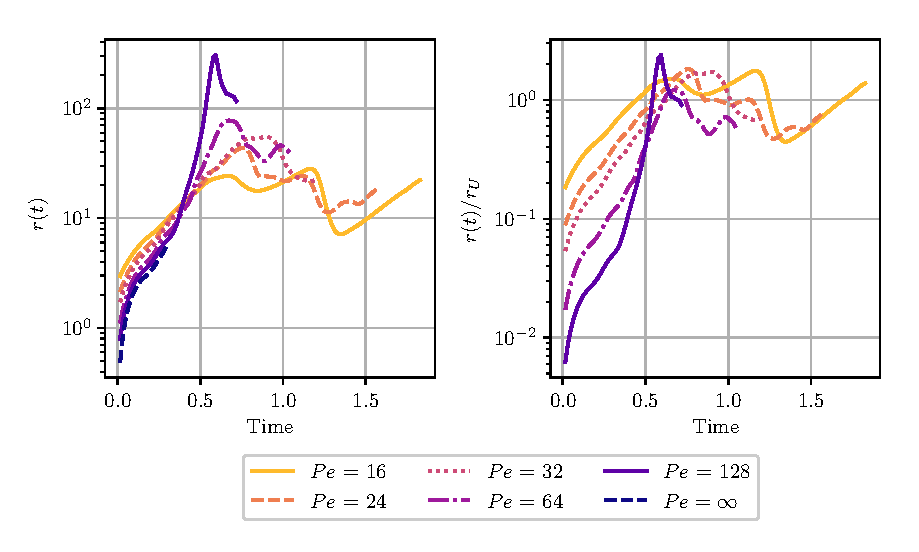
\includegraphics[]{ch-lit/images/energy_rate}
\caption{The left subplot shows the mixing rate $r(t)$ over time when subject to the optimal energy-constrained flow. The right subplot is the same data except scaled: $r(t)/r_{U} = r(t)/Pe$.}
\label{fig:energy_rate}
\end{figure}

 Figure \ref{fig:enstrophy_film} shows the evolution of a scalar field under the optimal flow for the enstrophy constraint. The top film strip corresponds to $Pe =\infty$ while the bottom is $Pe = 256$. The time evolution is initially similar but soon diverges over time. Figure \ref{fig:energy_film} shows the evolution for the energy constraint. The top film strip corresponds to $Pe =\infty$ while the bottom is $Pe = 32$. Notice that, unlike the $Pe = \infty$ cases, the flows with finite $Pe$ are incapable of creating length scales arbitrarily small for either the energy or enstrophy cases.  The left subplot of Figures \ref{fig:enstrophy_length} and \ref{fig:energy_length} shows this phenomena more quantitatively by showing $\lambda$ over time eventually reaching a plateau. The shell-model prediction of this limiting length scale is the Batchelor scale given by $\lambda_{\Gamma} = 1/\sqrt{Pe}$ for the enstrophy case and  $\lambda_{U} = 1/Pe$ for the energy case. The right plots of Figures \ref{fig:enstrophy_length} and \ref{fig:energy_length} shows scaled versions of $\lambda$ given by  $\lambda/\lambda_{\Gamma}$ and $\lambda/\lambda_{U}$ respectively.  Notice how they plateau around an $O(1)$ constant. Thus this result is consistent with the shell-model predictions. 
   
The mixing rates for the enstrophy case are shown in Figure \ref{fig:enstrophy_rate}. The rate during the transient phase is $\Gamma$ which is consistent with rates expected from $Pe=\infty$ mixing studies. For all $Pe$ considered, there is an increase in the rate of mixing after transient behaviour has finished to a long-term rate. Perhaps surprisingly, this long-term mixing rate appears to be {\it independent} of $Pe$ for fixed enstrophy. This suggests that the optimal long-term rate of mixing is only dependent on the rate-of-strain $\Gamma$ and not influenced by the strength of diffusion. 

It should be noted that the onset of the long-term rate is affected by the value of $Pe$. When there is strong diffusion (small $Pe$), the Batchelor scale is reached quickly. From the work of G. Iyer {\it et al.} \cite{GI2014} and C. Seis \cite{CS2013}, we know that $\lambda$ decreases at most exponentially for $Pe = \infty$. If we assume that the local-in-time optimal flows nearly saturate this bound in the transient phase, we model $\lambda$ as  $\lambda (t) = \lambda(0)\exp(- \alpha t) $ during this time. We expect the critical transition time $t_{c}$ that marks the end of this transient period to satisfy $\lambda(t_{c})= \lambda_{\Gamma}$. This time is theorized to be $t_{c}=\frac{1}{\alpha}\ln(\lambda(0)/\lambda_{\Gamma}) = \frac{1}{\alpha}\ln ( \sqrt{Pe} )$ for $Pe>1$ (If $Pe \leq 1$, then there is no transient phase). Hence, a smaller value of $Pe$ will result in an earlier onset of the long-term rate of mixing. Therefore, it is advantageous to have strong diffusion (small $Pe$) so that there is an earlier onset of the long-term mixing rate (although independent of $Pe$) which is an improvement over the mixing rate of the purely non-diffusive situation ($Pe=\infty$).
 
For the energy case, the long-term mixing rate decreases with decreasing $Pe$ (see the left subplot of figure \ref{fig:energy_rate}).  {\it Thus, strong diffusion results in a weak long-term mixing rate}. The right subplot of Figure \ref{fig:energy_rate} is $r/r_{U} =  r/Pe$. We see oscillations of $r/r_{U}$ around a value that is $O(1)$ which indicates that our numerical results are consistent with our predictions from the shell model. Thus, the long-term mixing rate is proportional to $Pe$ in contrast to the long-term mixing rate of enstrophy which carries no dependence on $Pe$.

For the energy case, the onset of the long run-mixing behaviour can be determined by the following model. From the work of E. Lunasin {\it et al.} \cite{JMP2012} on the fixed energy case, $\lambda(t)$ can decrease linearly in time to produce perfect mixing in finite time. We model the transient phase as $\lambda(t)=\lambda(0)(1-\beta t)$. Therefore, we theorize that the critical transition time is $t_{c}=\frac{1}{\beta}(1 -\lambda_{U}/\lambda(0)) = \frac{1}{\beta}(1 - 1/Pe)$ with $Pe> 1$ (If $Pe \leq 1$, there is no transient phase) for the energy case. Thus, it is true that one can still achieve an earlier onset of the long-term mixing behaviour by choosing a smaller $Pe$. However, an earlier onset time is accompanied by a slower long-term mixing rate. As for choosing a large $Pe$, the onset time is bounded above by $\frac{1}{\beta}$ and results in a faster long-term mixing rate. Thus, it is advantageous to have weak diffusion (large $Pe$) for mixing in the fixed energy case. This benefit is well illustrated by $H^{-1}$ norm in figure \ref{fig:energy_norms}. Notice that the mixing rate is initially slow for $Pe = 512$ but then out competes the mixing rate of smaller values of $Pe$.    

%%%
%%%
%%% DISCUSSION 
%%%
%%%

\section{Discussion}
\label{sec:discussion}
%
The local-in-time optimization results suggest that there is a limiting length scale for passive tracer mixing whenever $L^{2}$ flows (either $\ltwo{\mathbf{u}}$ or $\ltwo{\nabla\mathbf{u}}$) are instantaneously optimized to decrease the $H^{-1}$ norm. The bounds derived under both $L^{\infty}$ constrained flow assumptions did not result in proving this observation, but they did definitively rule out the possibility of perfect mixing in finite time for these $L^{\infty}$ flow constraints. 

We suspect that the bounds obtained for $L^{\infty}$ flows are not sharp and could be improved further. The $L^{\infty}$ flow analysis produced a double-exponential lower bound on the $H^{-1}$ norm rather than exponential as possibly expected given the numerical results for local-in-time optimal $L^2$ flows. The double-exponential bounds arise from the use of exponential upper bounds on the quantity $\frac{\hone{\theta}}{\ltwo{\theta}}$ in time for both $L^{\infty}$ flow constraints considered. We surmise that in fact $\frac{\hone{\theta}}{\ltwo{\theta}} < C$ (where $C$ is a constant) for all time $t$ as suggested by the numerical results. If this is true generally for the $L^{\infty}$  flows, then our previous analysis would demonstrate that the $H^{-1}$ norm is bounded below by a single exponential instead of a double exponential.

Note that the pure diffusive case discussed in the introduction can always be employed as a mixing strategy by simply not having a flow field at all ($\vec{u} =\vec{0}$) provided that the flow intensity constraints are generalized to inequalities such as $\|\vec{u}\| \leq UL^{d/2}$ and $\|\nabla \vec{u}\| \leq \Gamma L^{d/2}$. This is a valuable strategy if one is content with mixing at a long-term rate of $\kappa k_{\min}^2$ where $k_{\min} = \min \{ |\vec{k}|  :  |\hat{\theta}_{\vec{k}}(0)| > 0  \}$. This may be advised in fact if $k_{\min} > 2 \pi / \lambda_{B}$. This may well be the most optimal strategy. Invoking a flow may cause the lower wave number modes to become `populated' and therefore may limit the mixing rate. It is important to keep this simple strategy in mind when trying to rigorously prove bounds on the $H^{-1}$ norm. This strategy has an important implication --- there does {\it not} exist a lower bound on the  $H^{-1}$ norm of the form $\hmone{\theta} \geq A e^{-rt}$ where  $r$ is independent of the initial data.

In the next chapter and future work, we will consider the optimal control problem with finite-time optimization to minimize the $H^{-1}$ norm at the end time rather than instantaneously attempting to minimize its decay rate. This might lead to flows that can produce even smaller length scales. In Miles and Doering \cite{Miles2017a}, finite-time optimization was explored in the context of the shell model where it was found that global-in-time and local-in-time optimization appeared to give similar mixing rates. For the shell model, however, the analysis was consistent with computation. In the partial differential equation case, the gap between analysis and computation remains to be closed.


%%%
%%%
%%% CONCLUSION 
%%%
%%%


\section{Conclusion}
\label{sec:conclusion}


Our numerical study of local-in-time optimization suggests that there is a limiting length scale, a generalized Batchelor length scale, which in turn determines a long-term mixing ``Batchelor rate". In dimensional form, this Batchelor rate was found to be proportional to $\Gamma$ for the fixed enstrophy case and $U^{2}/\kappa$ for the fixed energy case. These rates are consistent with those found in the context of the shell model. Although the Batchelor scale has been a theorized lower bound on the length scales present on turbulent flows, it has not been proven rigorously. We hope this numerical study provides insight and promotes investigation into mathematically proving what conditions are necessary on the flow for a length scale limitation. This is especially important since it plays a crucial role in the achievable mixing rates. Furthermore, we provided numerical evidence that (1), for fixed enstrophy optimal flows, strong diffusion can benefit from an early onset of a long-term mixing rate (where the rate itself however is independent of diffusion strength) while (2), for energy fixed optimal flows, strong diffusion weakens the long-term mixing rate. 

 


 
 \chapter{Global-in-time optimization}
 \label{chap:git}
 
\section{Introduction}

In this chapter,  we explore global-in-time or finite-horizon optimization. The objective is to maximize mixing  at a prescribed final time as oppose to instantaneously as before.  This optimization problem employs the techniques from calculus of variations and optimal control \cite{Kirk2004a, gelfand2000calculus, fox1950introduction,troltzsch2010optimal, bertsekas1995dynamic,liberzon2011calculus}. We will focus primarily on the enstrophy-constrained case but will explicitly mention when analogous results carry over to the energy-constrained problem.

This chapter is organized as follows. We introduce the theory and setup of the optimization problem in Section \ref{sec:git_theory}. This section introduces the associated Euler-Lagrange equations and total variation. Section \ref{sec:numerical_method} describes two numerical methods for solving the Euler-Lagrange equations. Lastly, analytical and numerical results are presented in Section \ref{sec:git_results} for the pure advective case ($\kappa = 0$).

This project is currently ongoing and the work done so far is presented. 
\section{Theory}
\label{sec:git_theory}
\subsection{The optimal control problem}
Here we describe the global-in-time optimization problem for enstrophy-constrained flows. Let $D=[0,L]^{d}$ be our domain where $L$ is the side length and $d$ is the total number of spatial dimensions. All functions defined on $D$ have periodic boundary conditions. We are interested in the following optimization problem:
\begin{equation}
	\label{eq:PDE_GIT}
	\min_{\mathbf{u}} \|\theta(\,\cdot\,,T)\|_{H^{-1}}^{2}
\end{equation}
subject to the constraints
\begin{equation}
	\label{eq:PDE_advection2-git}
	\partial_{t}\theta+\mathbf{u}\cdot \nabla \theta= \kappa \Delta \theta
\end{equation}
with 
\begin{equation}
\label{eq:PDE_divfree2-git}
\nabla \cdot \mathbf{u} = 0
\end{equation}
and a {\it time-averaged} enstrophy constraint
\begin{equation}
	\label{eq:PDE_enstrophy-git}
	\frac{1}{T}\int_{0}^{T}\int d^{d}x dt |\nabla\mathbf{u}|^{2} = \Gamma^2 L^{d}.
\end{equation}
In addition, we are provided with initial data
\begin{equation}
	\label{eq:PDE_initial_condition2-git}
	\theta(\mathbf{x},0)=\theta_{0}(\mathbf{x}).
\end{equation}
%
\subsection{First and total variation for enstrophy-constraint}

Calculus of variations provides the appropriate framework for investigating the conditions placed on optimizers of functionals. Here we present the first and total variation results for the enstrophy-constrained case with diffusion. Prior to presenting these results, it is useful to make the following definitions:

\begin{itemize}
\vspace{0.25 cm}

\item \noindent \textbf{Definition} The pair of functions $\{\theta^{*}(x,t), \mathbf{u}^{*}(x,t)\}$ on $D$ is said to be \textbf{admissible} if it satisfies the following constraints \[\partial_{t}\theta+\vec{u}\cdot \nabla \theta=\kappa \Delta \theta \]
\[\nabla\cdot \mathbf{u}=0\]
\[\int_{0}^{T}\int_{D}d^{d}xdt |\nabla \mathbf{u}|^{2}=\Gamma^2L^{d}T\] and the initial data $\theta(\mathbf{x},0)=\theta_{0}(\mathbf{x})$.

\vspace{0.25 cm}

\item \noindent \textbf{Definition} An admissible pair $\{\theta^{*}(\mathbf{x},t), \mathbf{u}^{*}(\mathbf{x},t)\}$ on $D$ is said to be an \textbf{optimal solution}, \textbf{minimizer}, or \textbf{minima} of the cost functional $C$ if the \textbf{total variation}
\[\Delta C=C\{\theta, u \}-C\{\theta^{*},u^*\} \] is non-negative for all admissible pairs $\{\theta,\mathbf{u}\}$.

\vspace{0.25 cm}

\noindent

\item \noindent \textbf{Definition} A pair $\{\theta(\mathbf{x},t), \mathbf{u}(\mathbf{x},t)\}$ on $D$ is said to be an \textbf{extrema} for the cost functional $C$ if the pair is admissible and the \textbf{first variation}
\[\delta C=\lim_{\epsilon\rightarrow0}\frac{C\{\theta+\epsilon\tilde{\theta},\mathbf{u} + \epsilon\tilde{ \mathbf{u}}\}-C\{\theta,\mathbf{u}\}}{\epsilon} \] vanishes.
\end{itemize}


It remains to be shown that a minimizer exists within the constrained set of velocity fields satisfying incompressibility and in the $H^1$ Sobolev space (required by the enstrophy constraint).  Is this a sufficient restriction to ensure that a minimizer exists? Proving the existence of a minimizer typically requires demonstrating weakly lower semicontinuity of the cost functional for a sufficiently restricted set of velocity fields. Furthermore, it remains to be shown that a minimizer is an extrema and thus must satisfy the Euler-Lagrange equations which require sufficient regularity of the cost functional. In the context of traditional calculus, this is analogous to ensuring that a minimizer of a function coincides with a point where the derivative is zero. Nevertheless, it is still worthwhile to solve the Euler-Lagrange equations for candidate solutions. To determine the Euler-Lagrange equations, we introduce the associated augmented Lagrangian
\begin{multline}
	\label{eq:PDE_lagrangian}
	\mathcal{L} = \frac{1}{2}\int_{D}d^{d}x |\nabla\Delta^{-1} \theta(\mathbf{x},T)|^{2}  +  \int_{D}d^{d}x \phi_0 (\theta(\mathbf{x},0)-\theta_0(\mathbf{x})) \\
	+ \int_{D} d^{d}x \int dt \left\{ \phi(\partial_{t}\theta+\mathbf{u}\cdot\nabla \theta - \kappa\Delta \theta) +\frac{\mu}{2} (|\nabla \times\mathbf{u}|^{2}- \Gamma^2) + p(\nabla\cdot \mathbf{u})
	\right \} 
\end{multline}
where $\phi_0, \phi, \mu, $ and $p$ are Lagrange multipliers introduced to enforce the system constraints. Assuming that a minimizer is an extrema, we find that a minimizer must satisfy the Euler-Lagrange equations:
\begin{subequations}
\label{eq:pde_first_variation_enstrophy}
\begin{equation}
	\label{eq:PDE_first_variation_1} 
	\frac{\delta \mathcal{L}}{\delta \theta(T)}=0 \quad \Rightarrow  \quad \Delta^{-1} \theta(\mathbf{x},T) - \phi(\mathbf{x},T) = 0 
\end{equation}
\begin{equation}
	\frac{\delta \mathcal{L}}{\delta \theta}=0 \quad \Rightarrow \quad\partial_{t}\phi + \mathbf{u}\cdot\nabla\phi   + \kappa \Delta \phi =0
	\label{eq:PDE_first_variation_2} 
\end{equation}
\begin{equation}
	\frac{\delta \mathcal{L}}{\delta  u}=0  \quad \Rightarrow  \quad   \phi \nabla\theta - \nabla p -\mu \Delta \mathbf{u}=0. \label{eq:PDE_first_variation_3}
\end{equation}
\begin{equation}
	\label{eq:PDE_first_variation_4}
	\frac{\delta \mathcal{L}}{\delta \phi}=0  \quad \Rightarrow  \quad  \partial_{t}\theta+\mathbf{u}\cdot \nabla \theta - \kappa \Delta \theta = 0
\end{equation}
\begin{equation}
\label{eq:PDE_first_variation_5}
\frac{\delta \mathcal{L}}{\delta p}=0 \quad \Rightarrow  \quad  \nabla \cdot \mathbf{u} = 0
\end{equation}
\begin{equation}
	\label{eq:PDE_first_variation_6}
\frac{\delta \mathcal{L}}{\delta \mu}=0 \quad \Rightarrow  \quad 	\int_{0}^{T}\int d^{d}x dt |\nabla \times \mathbf{u}|^{2} - \Gamma^2 L^{d}T = 0
\end{equation}
\begin{equation}
	\label{eq:PDE_first_variation_7}
\frac{\delta \mathcal{L}}{\delta \phi_0}=0 \quad \Rightarrow  \quad	\theta(\mathbf{x},0) - \theta_{0}(\mathbf{x}) = 0.
\end{equation}
\end{subequations}
Note that equation \ref{eq:PDE_first_variation_2} has the same analytic and numerical challenges as the backwards heat equation given the sign of diffusion term. As a consequence, this equation will be solved backwards in time in our numerical schemes presented in a later section.

%\subsubsection{Second and Total Variation}
%
%\begin{flushleft}
%
%Let $\theta(\mathbf{x},t)$ and $\mathbf{u}(\mathbf{x},t)$ be arbitrary functions on $D \times [0,T]$ and define a cost functional be
%\[
%C\{\theta\}=\| \theta(\mathbf{x},T)\|^{2}_{H^{-1}}=\int_{D}d\mathbf{x} |\nabla^{-1} \theta(\mathbf{x},T)|^{2}.\]
%
%Define the quantities:
%\begin{align*}
%g_{1}\{\theta,\mathbf{u}\} &= \partial_{t}\theta+\mathbf{u}\cdot \nabla \theta - \kappa \Delta \theta \\
%g_{2}\{\mathbf{u}\} &= \nabla\cdot \mathbf{u} \\
%g_{3}\{\mathbf{u}\} &= \int_{0}^{T}\int_{D}d\mathbf{x}dt |\nabla \mathbf{u}|^{2}-TL^{d}\Omega^{2}.
%\end{align*}
%
%Let $\phi(\mathbf{x},t),$ and $ q(\mathbf{x},t)$ be arbitrary functions on $D \times [0,T]$ and let $\mu$ be a scalar. Define the functional $G$ as
%
%\begin{equation}
%\label{eq:constraint-functional}
%G\{\theta,\mathbf{u},\phi,q,\mu\}=\iint [\phi(\mathbf{x},t) g_{1}\{\theta,\mathbf{u}\} + q(\mathbf{x},t) g_{2}\{\mathbf{u}\}]d\mathbf{x}dt+\mu g_{3}\{\mathbf{u}\}
%\end{equation}
%
%Let the pair $\{\theta_{0},\mathbf{u}_{0}\}$ be an extrema of $C$ and $\{\theta_{1},\mathbf{u}_{1}\}$ be an admissible pair. Note that since $\{\theta_{0},\mathbf{u}_{0}\}$ and $\{\theta_{1},\mathbf{u}_{1}\}$ are admissible, $G\{\theta_{0},\mathbf{u}_{0},\phi,q,\mu\}=0$ and $G\{\theta_{1},\mathbf{u}_{1},\phi,q,\mu\}=0$. Hence, the total variation of G is also zero,
%\[\Delta G= G\{\theta_{1},\mathbf{u}_{1},\phi,q,\mu\}-G\{\theta_{0},\mathbf{u}_{0},\phi,q,\mu\}=0.\]
%
%
% Let $\delta\theta=\theta_{1}-\theta_{0}$ and $\delta \mathbf{u}=\mathbf{u}_{1}-\mathbf{u}_{0}$.
% 
% \[\Delta G=\iint [\phi(\mathbf{x},t) g_{1}\{\theta_{1},\mathbf{u}_{1}\} + q(\mathbf{x},t) g_{2}\{\mathbf{u}_{1}\}]d\mathbf{x}dt+\mu g_{3}\{\mathbf{u}_{1}\}\]
%  \[-\iint [\phi(\mathbf{x},t) g_{1}\{\theta_{0},\mathbf{u}_{0}\} + q(\mathbf{x},t) g_{2}\{\mathbf{u}_{0}\}]d\mathbf{x}dt-\mu g_{3}\{\mathbf{u}_{0}\}\]
%  
%  \begin{eqnarray*}
% 	 &=& \iint [
%  		\phi\left(
%  			\partial_{t}(\theta_{0}+\delta\theta)+(\mathbf{u}_{0}+\delta\mathbf{u})\cdot \nabla(\theta_{0}+\delta\theta)
%  			-\partial_{t}\theta_{0}-\mathbf{u}_{0}\cdot \nabla 					\theta_{0}
%	  	\right) \\
%	&+& q\left(
%		\nabla\cdot(\mathbf{u}_{0}+\delta\mathbf{u})-\nabla\cdot\mathbf{u_{0}}	
%	  	\right) \\
%	&+&\mu \left( 
%		 	 |\nabla(\mathbf{u}_{0}+\delta\mathbf{u})|^{2}- |\nabla \mathbf{u}_{0}|^{2}
%	  	\right)
%  ]d\mathbf{x}dt
%\end{eqnarray*}
%
%  \begin{eqnarray*}
% 	\implies \Delta G &=& \iint \{
%  		(-\partial_{t}\phi-\mathbf{u}_{0}\cdot\nabla\phi)\delta\theta
%		+( \phi \nabla\theta_{0} - \nabla q -\mu \Delta \mathbf{u}_{0})\cdot \delta\mathbf{u} \\
%		 &+&\nabla\phi\cdot\delta\mathbf{u}\delta \theta 
%		 +\mu |\nabla\delta \mathbf{u}|^{2}  
%  		t\}d\mathbf{x}dt \\
%  &+& \int_{D}\phi(x,T)\delta\theta(x,T)d\mathbf{x} = 0
%\end{eqnarray*}
% 
%  
% 
%  Consider the total variation of C
% \[ \Delta C= C\{\theta_{1}\}-C\{\theta_{0}\} \] 
% \[=\int_{D}\left\{ |\nabla^{-1}\theta_{1}(\mathbf{x},T)|^{2} - |\nabla^{-1} \theta_{0}(\mathbf{x},T)|^{2} \right\} d\mathbf{x} \]
% 
%\[=\int_{D}\left\{ 
%  			|\nabla^{-1} \left[
%  				\theta_{0}(\mathbf{x},T)+\delta\theta(\mathbf{x},T)											\right]|^{2} 
%  			- |\nabla^{-1} \theta_{0}(\mathbf{x},T)|^{2} 
%  		\right\} 
%d\mathbf{x} \]
%  
%\[
%	=\int_{D}
%	\left\{ 
%   		\nabla^{-1}\theta_{0}(\mathbf{x},T)\cdot
%   		\nabla^{-1} \delta\theta(\mathbf{x},T)
%   		+|\nabla^{-1} 
%		\delta\theta(\mathbf{x},T)|^{2} 
%   \right\} 
%   d\mathbf{x}  
%\]
% 
%\[
%	=\int_{D}
%	\left\{ 
%   		-\Delta^{-1}\theta_{0}(\mathbf{x},T)\delta\theta(\mathbf{x},T)
%   		+|\nabla^{-1} 
%		\delta\theta(\mathbf{x},T)|^{2} 
%   \right\} 
%   d\mathbf{x}  
%\]
% 
%Since $\Delta G=0$, we can add  $\Delta G$ to $\Delta C$ without any consequence. Let the index ``$_{T}$'' be shorthand for the arguments $(\mathbf{x},T)$. (e.g. $\phi_{T}=\phi(\mathbf{x},T)$)
%
%
%  \begin{eqnarray*}
% 	\Delta C&=& \Delta C+\Delta G \\
% 	         &=& \iint \left\{
%  			(-\partial_{t}\phi-\mathbf{u}_{0}\cdot\nabla\phi)\delta\theta
%			+( \phi \nabla\theta_{0} - \nabla q -\mu \Delta \mathbf{u}_{0})\cdot \delta\mathbf{u}
%			 +\nabla\phi\cdot\delta\mathbf{u}\delta \theta 
%			 +\mu |\nabla\delta \mathbf{u}|^{2}  
%  		\right\}d\mathbf{x}dt \\
%		  &+& \int_{D}\left\{
%  			(\phi_{T}-\Delta^{-1}\theta_{0,T})\delta\theta_{T}
%   			+|\nabla^{-1} 
%			\delta\theta_{T}|^{2}
%	       \right\} d\mathbf{x}		
%\end{eqnarray*}
% 
%
%Assuming that the global optimizer has vanishing first variation, we must show that the second variation (all quadratic terms of perturbations) is nonnegative for a candidate global minimum. For the moment suppose that the first variation vanishes, then 

We highlight that \ref{eq:pde_first_variation_enstrophy} provides necessary, but not sufficient, conditions for an optimal solution. To prove optimality, it suffices to show the total variation at an extrema (see Appendix \ref{sec:variation_calc} for calculation details)
  \begin{eqnarray}
  	\label{eq:total_Variation}
 	\Delta C&=& \iint \left\{\nabla\phi\cdot\delta\mathbf{u}\delta \theta 
			 +\mu |\nabla\delta \mathbf{u}|^{2}  
  		\right\}d\mathbf{x}dt +\int_{D}
  			|\nabla^{-1} 
			\delta\theta_{T}|^{2}
	      d\mathbf{x} \geq 0
\end{eqnarray}
%
for all perturbations $\delta\theta = \tilde{\theta}-\theta$ and $\delta \mathbf{u} = \tilde{\mathbf{u}}-\mathbf{u}$ about the candidate solution $\{\theta,\mathbf{u}\}$ where $\{\tilde{\theta},\tilde{\mathbf{u}}\}$ is admissible. That said, this is a non-convex optimization problem so this is not a trivial task.

%\end{flushleft}

\subsection{First and total variation for energy constraint}
The analysis for the energy-constrained problem with $\frac{1}{T}\int_{0}^T\ltwo{\mathbf{u}}^2 = U^2L^2$ is similar to that for the enstrophy-constrained problem. Here we simply state the analogous results. The augmented Lagrangian for energy constrained problem is 
\begin{multline}
	\label{eq:PDE_lagrangian}
	\mathcal{L} = \frac{1}{2}\int_{D}d^{d}x |\nabla\Delta^{-1} \theta(\mathbf{x},T)|^{2}  +  \int_{D}d^{d}x \phi_0 (\theta(\mathbf{x},0)-\theta_0(\mathbf{x})) \\
	+ \int_{D} d^{d}x \int dt \left\{ \phi(\partial_{t}\theta+\mathbf{u}\cdot\nabla \theta ) +\frac{\mu}{2} (|\mathbf{u}|^{2}- U^2) + p(\nabla\cdot \mathbf{u})
	\right \} .
\end{multline}
%
The Euler-Lagrange equations are
\begin{subequations}
\begin{equation}
	\label{eq:PDE_first_variation_1_energy} 
	\frac{\delta \mathcal{L}}{\delta \theta(T)}=0 \quad \Rightarrow  \quad \Delta^{-1} \theta(\mathbf{x},T) - \phi(\mathbf{x},T) = 0 
\end{equation}
\begin{equation}
	\frac{\delta \mathcal{L}}{\delta \theta}=0 \quad \Rightarrow \quad\partial_{t}\phi + \mathbf{u}\cdot\nabla\phi   + \kappa \Delta \phi =0
	\label{eq:PDE_first_variation_2_energy} 
\end{equation}
\begin{equation}
	\frac{\delta \mathcal{L}}{\delta  u}=0  \quad \Rightarrow  \quad   \phi \nabla\theta - \nabla p +\mu \mathbf{u}=0. \label{eq:PDE_first_variation_3_energy}
\end{equation}
\begin{equation}
	\label{eq:PDE_first_variation_4_energy}
	\frac{\delta \mathcal{L}}{\delta \phi}=0  \quad \Rightarrow  \quad  \partial_{t}\theta+\mathbf{u}\cdot \nabla \theta - \kappa \Delta \theta = 0
\end{equation}
\begin{equation}
\label{eq:PDE_first_variation_5_energy}
\frac{\delta \mathcal{L}}{\delta p}=0 \quad \Rightarrow  \quad  \nabla \cdot \mathbf{u} = 0
\end{equation}
\begin{equation}
	\label{eq:PDE_first_variation_6_energy}
\frac{\delta \mathcal{L}}{\delta \mu}=0 \quad \Rightarrow  \quad 	\int_{0}^{T}\int d^{d}x dt |\mathbf{u}|^{2} - U^2 L^{d}T = 0
\end{equation}
\begin{equation}
	\label{eq:PDE_first_variation_7_energy}
\frac{\delta \mathcal{L}}{\delta \phi_0}=0 \quad \Rightarrow  \quad	\theta(\mathbf{x},0) - \theta_{0}(\mathbf{x}) = 0
\end{equation}
\end{subequations}
%
and the total variation at an extrema is 
  \begin{eqnarray}
  	\label{eq:total_Variation_energy}
 	\Delta C&=& \iint \left\{\nabla\phi\cdot\delta\mathbf{u}\delta \theta 
			 +\mu |\delta \mathbf{u}|^{2}  
  		\right\}d\mathbf{x}dt +\int_{D}
  			|\nabla^{-1} 
			\delta\theta_{T}|^{2}
	      d\mathbf{x}
\end{eqnarray}
for all perturbations $\delta\theta = \tilde{\theta}-\theta$ and $\delta \mathbf{u} = \tilde{\mathbf{u}}-\mathbf{u}$ about the candidate solution $\{\theta,\mathbf{u}\}$ where $\{\tilde{\theta},\tilde{\mathbf{u}}\}$ is admissible. 
%
\subsection{Optimal control problem with inequality constraints}
One may be interested in the following {\it inequality} constraint on $\mathbf{u}$ in place of equations \eqref{eq:PDE_enstrophy-git}:
%
\begin{equation}
	\label{eq:PDE_enstrophy-git-ineq}
	\int_{0}^{T}\int d^{d}x dt |\nabla \times \mathbf{u}|^{2} \leq \Gamma^2 L^{d}T
\end{equation}
%
This formulation allows for the possibility of not consuming the entire stirring budget. Intuitively, this seems an unlikely scenario since it seems inefficient not to use of one's stirring resources. We provide the following argument that the inequality constraint is likely saturated for $\kappa = 0$ but not necessarily for $\kappa \neq 0$.

Consider the enstrophy constraint with $\kappa = 0$. Suppose $\{\theta^{*}, u^{*}\}$ are minima where \eqref{eq:PDE_enstrophy-git-ineq} is not saturated and $\int_{0}^{T}\int d^{d}x dt |\nabla \times \mathbf{u}|^{2} = m \Gamma^2 L^{d}T$ with $0\leq m <1$. Then one can construct new variables $\tilde{\theta},\tilde{\mathbf{u}}$ as  $\tilde{\theta}(\mathbf{x},t) = \theta^{*}(\mathbf{x},ct)$ and $\tilde{\mathbf{u}}(\mathbf{x},t) =c u^{*}(\mathbf{x},ct)$ defined for $t\in [0,T/c]$.  Any intermediate $c$ ($1< c < \frac{1}{m}$) will produce the original final-time mix-norm value but at an earlier time $t= T/c$ with available budget $(1-c^2m^2)\Gamma^2L^dT$ left over. Therefore, if there exists {\it any} $\mathbf{u}$ defined for the remaining time ($t\in [T/c,T]$) that is able to decrease the mix-norm by even the slightest amount with budget remaining, then this new candidate solution ($\tilde{\mathbf{u}}$ for $t\in [0,T/c]$ and  $\mathbf{u}$ for $t\in [T/c,T]$) defeats the supposed minima $\{\theta^{*}, \mathbf{u}^{*}\}$.  The instantaneous optimal strategy from the previous chapter is a good candidate, however there are cases where the first derivative of the mix-norm can not be controlled. This case must be dealt with to make this argument rigorous. 

Nevertheless, it still remains worthwhile to formulate the inequality-constrained optimal control problem. We may have confidence that the bound is saturated in the $\kappa =0$ case (given the argument above), but it not obvious that it will always be saturated with diffusion. In fact, there are trivial cases where $\mathbf{u} = 0$ is a reasonable choice. Consider the enstrophy case with initial data $\theta(\mathbf{x},0)$ given by a Fourier mode with large wavenumber $k_0$ and with a corresponding wavelength that is much smaller than the Batchelor wavenumber $k_{B} = \sqrt{\Gamma/\kappa}$. If $\mathbf{u} = 0$, then the advection-diffusion equation becomes simply the diffusion equation, and the mix-norm exhibits exponential decay with rate $-\kappa k_0^2$. However from the local-in-time optimization study of the previous chapter, we found that when advection and diffusion are both actively attempting to minimize the mix-norm, the scalar field develops length scales comparable to the Batchelor scale in the long run. Therefore, a rough approximation of the long-term exponential rate is likely to be $-\kappa k_{B}^2 = -\Gamma$. Therefore in the case were $\Gamma < \kappa k_0^2$, then $\mathbf{u} = 0$ may be a reasonable choice. In other words, stirring (when $\mathbf{u}\neq 0$) may move some spectral mass to wave numbers less than the Batchelor wavenumber and be disruptive. This argument gives reason to believe that the optimal strategy may not always benefit from saturation of the budget.


%\subsubsection{Calculus of variations}
%
% We generalize the results of \cite{Forster1978} here.
 
 

%\subsection{Hamiltonian formulation}
%
%
%
%\subsection{Finite-dimensional forms of optimization problem}
%
%The optimization problem of the previous section can be viewed as optimization of a cost with control of an infinite dimensional vector (a function). In practice, it is worthwhile to consider finite forms of the optimization problem presented since the optimization problem will inevitably be solved in this form on a computer. 
%
%In addition, we will gain value by applicability of Hamiton-Jacobi-Bellmann equation and Dynamic Programming.  We will demonstrate that even in the finite dimensional setting the full Dynamic Programming task is still challenging. There are only a select set of examples where the Hamilton-Jacobi-Bellman equation can be solved exactly (such as in the canonical linear-quadratic regulator problem). Its analog in the original problem (if it can even be well-posed) would be an even more challenging task since the analog of the Hamilton-Jacobi-Bellman equation would likely take the form of a variational equation with a functional as a solution. 
%
%The full Hamilton-Jacobi-Bellman equation in the finite form in most cases suffers from the `curse of dimensionality'. Fortunately, there are approximation methods --- the field exploring these methods is known as Approximate Dynamic Programming (also known as Neurodynamic programing and Reinforcement Learning). We will explore these in later sections.
%
%There are two paths to finite-dimensionality reduction: one could optimize first and then reduce or reduce first and then optimize. We will first consider the latter. By optimize, I mean derive the necessary Euler-Lagrange equations. This was done in the previous section. The next step would be to then reduce the dimensionality of these equations in space and time. We will do this step in sequence by first looking at the consequence of reductions in space. 
%
%
%The spatial dimensionality reduction is done by a spectral decomposition into Fourier modes (an appropriate choice due to periodic conditions). The state equation (advection-diffusion equation) in Fourier space is expressed as 
%\begin{equation}
%\label{eq:advection_spectral}
%\partial_{t}\hat{\theta}(\mathbf{k},t)+i\sum_{\mathbf{k}'}\hat{u}(\mathbf{k}-\mathbf{k}',t)\cdot \mathbf{k}' \hat{\theta}(\mathbf{k}',t)+\kappa |\mathbf{k}|^2\theta(\mathbf{k},t)=0
%\end{equation}
%or 
%\begin{equation}
%\label{eq:advection_spectral_condensed}
%\partial_{t}\hat{\theta}(\mathbf{k},t)=i\sum_{\mathbf{k}'}A_{\mathbf{k},\mathbf{k}'} \hat{\theta}(\mathbf{k}',t)-\kappa |\mathbf{k}|^2\theta(\mathbf{k},t)
%\end{equation}
%where 
%\begin{equation}
%A_{\mathbf{k},\mathbf{k}'}=-\hat{u}(\mathbf{k}-\mathbf{k}',t)\cdot \mathbf{k}'.
%\end{equation}
%One can show that $A$ is hermitian ($A=A^{\dagger}$). Note that the above representation is {\it exact} as an infinite system of ordinary differential equations --- no dimensionality reduction so far. Letting $M = K^{-1}K^{-1}$, $K_{\mathbf{k},\mathbf{k}'} = \mathbf{k} \mathds{1}_{\mathbf{k}=\mathbf{k}'}, A = \sum_{\mathbf{k}} \mathbf{\hat{u}}(\mathbf{k}) B(\mathbf{k})$, and $B(\mathbf{k}'')_{\mathbf{k},\mathbf{k}'} = -i\mathbf{k}'\mathds{1}_{\mathbf{k}''=\mathbf{k}'-\mathbf{k}}$, we can write can write the spectral version of the Euler-Lagrange equations as (in matrix form)
%\begin{subequations}
%	\begin{align}
%	\label{eq:matrix_terminal-git}
%	 M\theta(T) - \phi(T) = 0 \\
%	 \label{eq:matrix_adj-git}
%	 \dot{\phi} - A\phi - \kappa K^2\phi= 0	\\
%	 \label{eq:matrix_state-git}
%	 \dot{\theta} - A\theta  - \kappa K^2\theta = 0	\\
%	 \label{eq:matrix_opt-git}
%	 \phi^{T}B(\mathbf{k})\theta + \mu |\mathbf{k}|^2 u(\mathbf{k}) = 0 \\
%	 \frac{1}{T}\int_{0}^T (u^{T}K^{2}u - \Gamma) = 0 \\
%	 \mathbf{k} \cdot u(\mathbf{k}) = 0
%	\end{align}
%	\label{eq:spectral_euler_lagrange}
%\end{subequations}
%where the hatted and bold face has been removed for the state $\theta$, adjoint $\phi$,  and control variables $u$ for clarity. 
%
%Now the discretized system simply follows as a Galerkin truncation of the spectral Euler-Lagrange equations \eqref{eq:spectral_euler_lagrange} above. We choose the truncation where all spectral components with $\|\mathbf{k}\|_{\infty} \leq a $ are kept with a corresponding number $N$ of total Fourier modes in each spatial dimension. Thus giving a total of $N^d$ fourier modes for $d$ spatial dimensions. This will cause a reduction of the matrices $M$, $K$, and $B$ above. Also $A$ becomes  $A = \sum_{\|\mathbf{k}\|_{\infty} \leq a} \mathbf{\hat{u}}(\mathbf{k}) B(\mathbf{k}).$
%
%
%Let's consider the other route to discretization mentioned earlier where we discretize first and then optimize. If we start with the spectral representation as our starting point, the truncation of the state equation and constraints lead to exactly the same expressions derived by the first approach. What remains are the associated equations governing the Lagrange multipliers. To determine these remaining relations, we must find the first variations of the following augmented Lagrangian
%\begin{multline*}
%	\mathcal{ L} \{ \theta, u,\phi,\mu \} = \frac{1}{2} \sum_{\|\mathbf{k}\|_{\infty}<a}^{}\frac{|\theta_{\mathbf{k}}(T)|^2}{|\mathbf{k}|^2} + \int_{0}^{T}\Bigg \{\sum_{\|\mathbf{k}\|_{\infty}<a}^{}\phi_{\mathbf{k}}(t)\left( \dot{\theta} - A\theta  - \kappa K^2\theta \right)_{\mathbf{k}} \\
%	\sum_{\|\mathbf{k}\|_{\infty}<a}q_{\mathbf{k}}(t)\mathbf{k} \cdot u(\mathbf{k}) +  \frac{\mu }{2}\left( u^{T}K^{2}u - \Gamma\right)  \Bigg\}\: dt
%\end{multline*}
%
%We find that the first variation of the above augmented lagrangian results in an identical set of equations derived in the first approach.
%
%We have however, only dealt with the reduction of the systems spatially. To also discretize in time, we have a choice of many numerical integration schemes. We will consider only 1-step numerical schemes of the form: $\theta^{m+1} = f(\theta^{m},u^{m})$ for $m = 1,2, \dots, M $.
%

\section{Numerical method for pure advection ($\kappa = 0$)}
\label{sec:numerical_method}

\subsection{Gradient descent algorithm}
%We perform the following update to $u$ by a conjugate-gradient scheme. At each time step $i$, the preconditioned gradient is given by  $\nabla_{u} J = - (\tilde{u}^{i} - u^{i})$ where $\tilde{u}^{i}$ solves the optimality condition \eqref{eq:matrix_opt-git} after integrating the state equation \eqref{eq:matrix_state-git} forward in time to find $\theta^{i}$ and adjoint equation  \eqref{eq:matrix_adj-git}  backwards in time to find $\phi^{i}$ with using the terminal condition \eqref{eq:matrix_terminal-git}. 
%

Here we describe a numerical method for solving the Euler-Lagrange equations \eqref{eq:PDE_first_variation_1} -- \eqref{eq:PDE_first_variation_7} corresponding the enstrophy-contained problem in 2 dimensions. We use a gradient-based method with line search. The overall strategy is to solve \eqref{eq:PDE_first_variation_1} -- \eqref{eq:PDE_first_variation_7} per iteration except \eqref{eq:PDE_first_variation_3}. The left hand side of \eqref{eq:PDE_first_variation_3} is in fact the gradient of the cost with respect to the velocity field over space and time that is valuable for our iterative update scheme on $\mathbf{u}$. To see that this is the gradient, consider the first variation of the entire augmented functional. If all first variations vanish except the variation with respect to $\mathbf{u}$, then
%
  \begin{eqnarray*}
 	\delta \mathcal{L}&=&  \iint ( \phi \nabla\theta - \nabla p -\mu \Delta \mathbf{u})\cdot \delta\mathbf{u} \,\, d\mathbf{x}dt .
\end{eqnarray*}
%
If in addition ${\theta + \delta\theta,u+ \delta u}$  remains admissible, then 
\begin{equation}
\label{eq:gradient-relation}
\frac{\delta C}{\delta \mathbf{u}} = \frac{\delta L}{\delta \mathbf{u}}=  \phi \nabla\theta - \nabla p -\mu \Delta \mathbf{u}
\end{equation}
for variations respecting the constraints. 

We discretize space as an $N$ by $N$ grid and time from $0$ to $T$ uniformly with $M$ time points. Thus, $\mathbf{u}$ is an array of shape $(M,2,N,N)$. $\theta$ and $\phi$ are arrays of shape $(M,N,N)$. The approach requires satisfying all the Euler-Lagrange equations except \eqref{eq:PDE_first_variation_3} per iteration. The update is of the following form:
\begin{equation}
\label{eq:update}
\mathbf{u}^{k+1} = \mathds{N}\left(\mathbf{u}^{k} - \eta \frac{\delta C}{\delta \mathbf{u}}(\mathbf{u}^{k})\right).
\end{equation}
where $\eta$ is the step size. Note that this updates the velocity field at all points of space and time. $\mathds{N}(\mathbf{v})$ enforces the enstrophy constraint: it is defined as $\mathds{N}(\mathbf{v}) = \alpha \mathbf{v}$ where $\alpha$ is a normalizing factor and chosen so $\frac{1}{T}\int_0^Tdt\|\nabla \mathds{N}(\mathbf{v}) (\,\cdot\, ,t)\|_{2}^2 = \Gamma^2 L^2 $.

To calculate $\frac{\delta C}{\delta \mathbf{u}}(\mathbf{u}^{k}) =  \phi^{k} \nabla\theta^{k} - \nabla p^{k} -\mu^{k} \Delta \mathbf{u}^{k}$, we must find $\theta^{k}, \phi^{k},\mu^{k}$ and $p^{k}$. $\theta^{k}$ is determined at each iteration from $\mathbf{u}^{k}$ by integrating the advection-diffusion equation with initial condition $\theta_0$. Then the terminal condition $\phi^{k}(\mathbf{x},T) = \Delta^{-1} \theta^{k}(\mathbf{x},T)$ is used to provide an `initial condition' for $\phi^{k}$. The velocity $\mathbf{u}^{k}$ is used to evolve adjoint equation for $\phi^{k}$ backwards in time given $\phi^{k}(\mathbf{x},T).$ Both integrations forward and backwards in time are done with a Fourier basis with $N$ modes to represent the spatial domain and a 2nd order Heun's time-stepping method. $N$ is chosen sufficiently large to to resolve spatially for all time. $dt $ is chosen small enough to satisfy both advective and diffusive CFL conditions. This criteria is compactly stated as $dt=0.25\min[1/(\Gamma N),L^2/(\kappa N^2)]$.  If we demand that the updated $\mathbf{u}^{k+1}$ be incompressible, then this requires that $\frac{\delta C}{\delta \mathbf{u}}(\mathbf{u}^{k})$ be incompressible. Towards this goal, we take the divergence of both sides of \eqref{eq:gradient-relation} and require that it vanish. This gives the following choice of $p^{k} = \Delta^{-1} \nabla \cdot (\phi^k \nabla \theta^k)$ which is equivalent to applying the divergence-free projection operator $\mathds{P}$ to $\frac{\delta C}{\delta \mathbf{u}}(\mathbf{u}^{k})$ where the projector $\mathds{P}(\mathbf{v})$ is defined as $\mathds{P}(\mathbf{v}) = \mathbf{v} - \nabla\Delta^{-1}(\nabla \cdot \mathbf{v})$. Lastly $\mu^{k}$ is chosen so that the update obeys the enstrophy constraint. This restriction is captured in the condition $\int_0^T\int_{D}\Delta \mathbf{u} \cdot \delta \mathbf{u}^k d\mathbf{x}dt= 0$ where $\delta \mathbf{u} = \mathbf{u}^{k+1} - \mathbf{u}^{k}$. According to our update and for small $\delta \mathbf{u}$ or equivalently $\eta$, this is approximately  given by $\delta \mathbf{u} \approx \eta\frac{\delta C}{\delta \mathbf{u}}(\mathbf{u}^{k}).$ We then calculate:
\begin{eqnarray}
\label{eq:linearized_constraint}
0 &=& \int_0^T\int_{D}d\mathbf{x}dt \, \Delta \mathbf{u}^{k} \cdot \delta \mathbf{u} \\
&=& \eta \int_0^T\int_{D}d\mathbf{x}dt \, \Delta \mathbf{u}^k \cdot ( \phi^k \nabla\theta^k- \nabla p^{k} -\mu^{k}\Delta \mathbf{u}^{k}) \\
&=&  \eta \int_0^T\int_{D}d\mathbf{x}dt \, \Delta \mathbf{u}^k \cdot (\mathds{P}(\phi^k \nabla\theta^k) -\mu^{k} \Delta\mathbf{u}^{k}) \\
 \end{eqnarray}
Therefore, we find that 
\begin{equation}
\mu^{k} =\frac{ \int_0^T\int_{D}d\mathbf{x}dt \, \Delta \mathbf{u}^k  \cdot \mathds{P}(\phi^k \nabla\theta^k)}{ \int_0^T\int_{D}d\mathbf{x}dt \, \Delta \mathbf{u}^k  \cdot \Delta \mathbf{u}^k }.
\end{equation}
This choice $\mu^{k}$ is chosen to enforce the enstrophy constraint. Note that \eqref{eq:linearized_constraint} is the {\it linearized} constraint condition. This is why we enforced this constraint by introducing the normalizing operator $\mathds{N}()$. The method as a whole is summarized in Figure \ref{fig:GD-algorithm}.  

We perform the following validation of the gradient by considering its projection onto the search direction $\mathbf{d} = - \frac{\delta C}{\delta \mathbf{u}}$ at $\mathbf{u}$ (chosen to be local-in-time velocity field).  We first computing the directional analytical gradient by 
\begin{equation}
G_{a} =\frac{ \int_0^T\int_{D}d\mathbf{x}dt \, \frac{\delta C}{\delta \mathbf{u}} \cdot \mathbf{d} }{ \int_0^T\int_{D}d\mathbf{x}dt \,  \mathbf{d}\cdot \mathbf{d} }.
\end{equation} 
and the finite-difference approximation with step $\epsilon$ given by 
\begin{equation}
G_{\epsilon} = \frac{C(\mathbf{u} + \epsilon\mathbf{d})- C(\mathbf{u} - \epsilon\mathbf{d})}{2\epsilon}
\end{equation} 
We can then compare the analytic gradient $G_{a}$ and its approximation $G_{\epsilon}$ to find the relative error $R$ defined as 
\begin{equation}
R = \frac{|G_{a}-G_{\epsilon}|}{|G_{a}|} 
\end{equation}
as function of $\epsilon$ as shown in figure \ref{fig:gradient}. Note that we get a decay in the relative error with smaller $\epsilon$ which eventually plateau to $R \approx 10^{-3}$ which is likely due to truncation error associated with our choices of $N$ and $M$. If $N$ and $M$ are increased, we would expect this saturated plateau to decrease. Improvements to determining an accurate gradient will be investigated further since it is important to have an accurate gradient for an efficient gradient descent search.



\begin{figure}

\begin{algorithmic}[1]
\Function{Gradient\_Descent($u_0$,$\theta_0$,\textit{tol})}{}
\State$u$ $\gets$ zeros array of shape (M,2,N,N)
\State $\theta$ $\gets$ zeros array of shape (M,N,N)
\State $\phi$ $\gets$ zeros array of shape (M,N,N)
\State
\State $u[0]$ $\gets$ $u_0$
\State
 \While {$\|\frac{\delta C}{\delta u}\| \geq tol$}
	\State  $\theta$ $\gets$ integrate\_forward($u$ ,$\theta_0$)
	\State  $\phi[M-1]$  $\gets  \Delta^{-1}(\theta[M-1]$)
	\State $\phi$ $\gets$ integrate\_backward($u$ ,$\phi[M-1]$)
	\State
	\State  $\frac{\delta C}{\delta u} \gets$ compute\_gradient($\theta,\phi,u$)
	\State  $d \gets  $divergence\_free\_projection($-\frac{\delta C}{\delta u} $)
	\State $\eta  \gets$ line\_search($u$,$d$)
	\State $u \gets$ normalize($u + \eta d$)
\EndWhile
\State	
\Return $u$
\EndFunction
\end{algorithmic}
\caption{Gradient descent for final-time optimization}
\label{fig:GD-algorithm}
\end{figure}

\begin{figure}
\centering
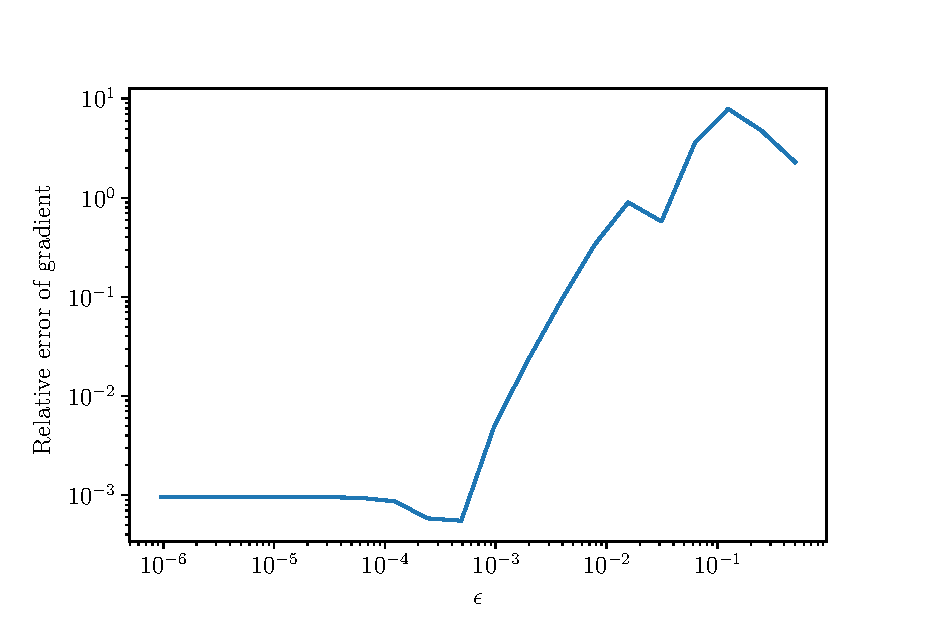
\includegraphics[width=0.7\textwidth]{ch-git/images/gradient}
\caption{The relative numerical error between analytical and finite-difference gradient as a function of the finite-difference step size $\epsilon$.}
\label{fig:gradient}
\end{figure}

\subsection{Target algorithm}
\label{sec:target_method}
The previous gradient descent algorithm picks the search direction $d$ to be proportional to the negative gradient. Here we purpose a different search direction that has improved convergence at least demonstrated in practice for the problem of interest and parameters chosen. The update is
\begin{equation}
\label{eq:target_update}
\mathbf{u}^{k+1} = \mathds{N}(\mathbf{u}^k + \eta \mathbf{d}^k)
\end{equation}
where $\mathbf{d}^k = \mathbf{u}_{t}^k - \mathbf{u}^k$ and $\mathbf{u}_t^k$ is the `target' solution given by 
\begin{equation}
\mathbf{u}_t^k = \mathds{N}(\Delta^{-1} \mathds{P}(\phi^{k} \nabla \theta^{k})).
\end{equation}
$\phi^{k}$ and $\theta^{k}$ are determined by integrating forward and backwards in time with $\mathbf{u}^{k}$ as seen before in the gradient descent algorithm. The above expression can be viewed as the solution to $ \phi^{k} \nabla\theta^{k} - \nabla p^{k} -\mu^{k} \Delta \mathbf{u}^{k}_t= 0$ where the $\mathbf{u}_t^{k}$ takes the place of $\mathbf{u}^{k}$ in the gradient expression while keeping $\theta^k$ and $\phi^{k}$ as solutions to the state and adjoint equations corresponding to $\mathbf{u}^{k}$. $\mu^{k}$ and $p^{k}$ are embodied in the normalization and divergence-free projection operators that require $\mathbf{u}_t^k$ to satisfy incompressibility and the intensity constraint. The algorithm is summarized in figure \ref{fig:target}.

\begin{figure}
\begin{algorithmic}[1]
\Function{Target($u_0$,$\theta_0$,\textit{tol})}{}
\State$u$ $\gets$ zeros array of shape (M,2,N,N)
\State $\theta$ $\gets$ zeros array of shape (M,N,N)
\State $\phi$ $\gets$ zeros array of shape (M,N,N)
\State
\State $u[0]$ $\gets$ $u_0$
\State
 \While {$\|d\| \geq tol$}
	\State  $\theta$ $\gets$ integrate\_forward($u$ ,$\theta_0$)
	\State  $\phi[M-1]$  $\gets  \Delta^{-1}(\theta[M-1]$)
	\State $\phi$ $\gets$ integrate\_backward($u$ ,$\phi[M-1]$)
	\State
	\State  $u_{target} \gets$ compute\_target($\theta,\phi,u$)
	\State  $d \gets  u_{target} - u$
	\State $\eta  \gets$ line\_search($u$,$d$)
	\State $u \gets$ normalize($u + \eta d$)
\EndWhile
\State	
\Return $u$
\EndFunction
\end{algorithmic}
\caption{Target algorithm for final-time optimization}
\label{fig:target}
\end{figure}



%
%\subsection{Hamilton-Jacobi-Bellman equation}
%So far, we have discussed only variational approach to optimal control. Here we introduce a dynamic programming perspective. The Hamilton-Jacobi-Bellman equation is given by 
%
%\begin{equation}
%\frac{\partial}{\partial t} V(\theta,t) = \min_{u}\left\{ \sum_{\mathbf{k}} \frac{\partial V(\theta, t)}{\partial \theta_{\mathbf{k}}} \frac{\partial \theta_{\mathbf{k}}}{\partial t}(\theta, u)\right\}
%\end{equation}
%with terminal condition $V(\theta,T) = \sum_{\mathbf{k}}\frac{|\theta_{\mathbf{k}}|^2}{|\mathbf{k}|^2}$ where $V(\theta,t): \mathds{C}^{N^d} \times [0,T] \rightarrow \mathds{R}$ and .
%
%As an aside, although the summation is over a finite set of $\mathbf{k}$ values, I speculate that the summation could just as well be over an infinite set of $\mathbf{k}$ for the full spectral formulation. In this case, $V$ is now a real-valued mapping over an infinite-dimensional vector space and hence is a functional. 
%
%Returning to the analysis of the reduced system, the time-discretized version is given by 
%\begin{equation}
%V^{n-1} (\theta)= \min_{u^{n-1}}\left\{ \sum_{\mathbf{k}} \frac{\partial V^{n}(\theta)}{\partial \theta_{\mathbf{k}}} f_{\mathbf{k}}(\theta, u)\right\}
%\end{equation}
%
%
%\subsection{Approximate Dynamic Programming}
%% \subsubsection{Instantaneous optimization as a one-step look ahead scheme} 
     
\section{Results for pure advection ($\kappa = 0$)}
\label{sec:git_results}
\subsection{Optimal budget use is uniform in time}
Recall that the velocity field is required to have a fixed {\it mean} enstrophy of $\Gamma$ over time. Surprisingly, we find that it is optimal to expend enstrophy uniformly in time. This is shown by the calculation using the Euler-Lagrange equations:
\begin{align*}
	\frac{d}{dt}\int_{D} d^{d}x | \nabla \times \mathbf{u} |^2 &= -\int_{D} d^{d}x \Delta\frac{\partial\mathbf{u}}{\partial t}\cdot \mathbf{u} \\
	&=- \frac{1}{\mu} \int_{D} d^{d}x \left(\frac{\partial\phi}{\partial t}\nabla \theta +\phi\nabla\frac{\partial\theta}{\partial t}  -\nabla \frac{\partial p}{\partial t} \right)\cdot \mathbf{u} \\
	&=- \frac{1}{\mu} \int_{D} d^{d}x \left(\frac{\partial\phi}{\partial t}\nabla \theta +\phi\nabla\frac{\partial\theta}{\partial t} \right)\cdot \mathbf{u} \\
	&=- \frac{1}{\mu} \int_{D} d^{d}x \left(\frac{\partial\phi}{\partial t}\mathbf{u} \cdot \nabla \theta -\mathbf{u} \cdot \nabla \phi\frac{\partial\theta}{\partial t} \right) \\
	&=0 
\end{align*}
Thus, enstrophy is utilized uniformly in time for a minimizer to problem (\ref{eq:PDE_GIT}) (provided that the minimizer satisfies the Euler-Lagrange equations).  This shows another commonality between the partial differential equation and shell model. A similar calculation reveals that energy is conserved in time for the energy-constrained problem.


\begin{figure}
\centering
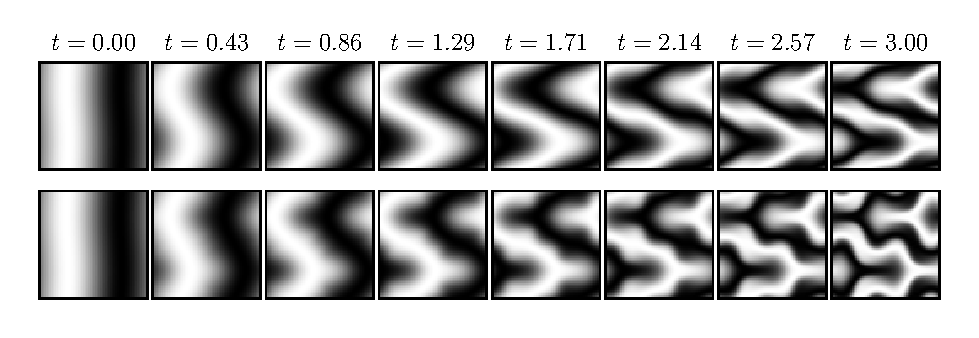
\includegraphics[width=\textwidth]{ch-git/images/output_N64_T3p0_gamma_1p0_kappa_0_L1p0/film.eps}
\caption{The top filmstrip is the local-in-time strategy while the bottom filmstrip is the global-in-time strategy. $\Gamma = 1.0$.}
\label{fig:lit_vs_git_film}
\end{figure}

\begin{figure}
\centering
\includegraphics[width=0.7\textwidth]{ch-git/images/output_N64_T3p0_gamma_1p0_kappa_0_L1p0/lit_vs_git_N64_T3p0_kappa0_L1_gamma1p0.eps}
\caption{The top subplot shows a comparison of local-in-time agains global-in-time optimization for fixed enstrophy ($\Gamma = 1.0$). The bottoms subplot shows uniform expenditure in time of the stirring budget as expected.}
\label{fig:lit_vs_git}
\end{figure}


\subsection{Comparison with local-in-time optimization}
We investigate the performance of global-in-time optimization relative to instantaneous optimization for $\Gamma =1.0$, $\kappa = 0$, $L=1.0$, $M=1000$, $N=64$ and $T=3.0$. We consider the performance of mixing the initial condition $\theta_0(\mathbf{x}) = \sin( 2\pi x/L).$ We use the numerical scheme described in section \ref{sec:target_method}. Python code is provided in Appendix \ref{app:git_code}. The resulting flow is shown in the bottom filmstrip of Figure \ref{fig:lit_vs_git_film} while the local-in-time flow is shown in the top filmstrip for comparison. Quantities of interests for this global-in-time optimal flow are shown in Figure \ref{fig:lit_vs_git}. The top subplot of Figure \ref{fig:lit_vs_git} shows how the $H^{-1}$ mix-norm varies in time. Note how initially the local-in-time flow outperforms the global-in-time optimal flow for short times, obviously due to the fact that it is a greedy algorithm maximizing mixing in the near future. However, note that the global-in-time flow eventually outperforms local-in-time by the final time as expected. Furthermore, observe that enstrophy is expended uniformly in time as expected by the previous analytical result.











 \chapter{Conclusion and Future Directions}
 \label{chap:conclusion}
 

% shell model
% Analytic results for 3 shell truncation
% Batchelor scale limitation
% Not much difference between lit and git

In this dissertation, new results on the optimization of mixing are uncovered. In the first study on optimization of a shell model, it is discovered that the mixing rate is limited by the presence of diffusion. We investigated both local- and global-in-time optimization for various shell model truncations. The 3-shell model was particularly informative since analytical solutions for Euler-Lagrange equations were obtained by using methods familiar to the theory of nuclear magnetic resonance. These analyses demonstrated clearly how the global-in-time optimization strategy  can outperform the local-in-time optimization scheme by a clever  `rotation' in state space.

In the local-in-time optimization study of the advection-diffusion equation, it is demonstrated numerically that a generalized Batchelor length scale places restrictions on the rate of mixing. Many other observations from the shell model also carried over to this setting.  For the enstrophy constrained problem, the long-term mixing rate is shown to be independent of diffusion coefficient. For the energy-constrained problem, we found that the mixing rate was dependent on diffusion coefficient in a perhaps surprising way --- increased diffusion can {\it decrease} the mixing rate as measured by the $H^{-1}$ norm. Diffusion is usually thought to benefit mixing as it tends to homogenize dye throughout a fluid, so its detrimental effect on the process is unexpected.

Finally, results are presented on our ongoing project on global-in-time optimization. In this study, we found that it is optimal to use the stirring budget uniformly in time when we only demanded that the {\it time-averaged} enstrophy be a desired fixed value. We also found this to be the case for the energy-constrained problem. This is consistent with the work of G. Mathew {\it et al.} \cite{GM2005} that found a uniform use of the stirring budget when controlling a superposition of a restricted set of enstrophy and energy constrained flows. We also presented the global-in-time strategy for a short time period which (as expected) outperformed the local-in-time strategy at the end time. However, the improvement is not dramatic in this short time period.


Global-in-time optimization is computationally challenging due to the large dimensionality of the search space. Improvements are being considered such as employing other gradient descent and line search methods. The primary bottleneck in the algorithm is the computation of gradient with respect to $\mathbf{u}$ (and equally true for the computation of the `target' velocity field) which requires time integration forwards and backwards in time. Methods for approximating this gradient would be valuable to speed up the computation, especially at earlier iterations where precision is not necessary until near the convergence point. The inclusion of diffusion will most likely require a formulation with inequality intensity constraints since it is not obvious that the intensity budget will be saturated given the argument of the previous chapter. In terms of future  theoretical and analytic work on global-in-time optimization, it is still important to determine the existence and uniqueness of optimizers for the presented problem. What function space restriction is necessary to ensure that a minimizer exists? 

These studies suggest the following questions to the mixing community:
\begin{itemize}
\item Can one demonstrate the mixing rate limitation of the Batchelor scale rigorously? What are the restrictions on the control $\mathbf{u}$ for this limitation to hold? Can one construct a flow that surpasses the Batchelor scale in the long-run?

\item Related to the previous question, can one derive a single exponential lower bound of the $H^{-1}$ norm with diffusion for energy or enstrophy stirring intensity constraints? Without diffusion, the rate is shown to depend on the support of the initial condition \cite{GI2014}. How does diffusion affect this dependence on the initial condition?
\end{itemize}


It is natural to ask ``Are optimal flows as defined feasible?" and ``How would one generate such flows in reality?" The purpose of this study is not to tackle these questions directly since our formulation is not entirely suitable for these questions. The purpose of this study is to consider idealized mixing to provide expectations in the best-case scenario with absolute control over the velocity field under the assigned constraints. In reality absolute control is generally not obtainable. 

Although we do not fully address feasibility in the series of studies presented here, we acknowledge that feasibility is an important issue and encourage research in this direction. With the goal of feasibility in mind, we can work backwards from a desired flow $\mathbf{u}$ to obtain the required forcing $\mathbf{f}$ on a fluid. This can be found by simply substituting a discovered (local- or global-in-time) optimal velocity field $\mathbf{u}$ into the Navier-Stokes equation to find:

\begin{equation}
\label{eq:ns}
\mathbf{f} = \rho\partial_{t} \mathbf{u}  + \rho\mathbf{u}\cdot \nabla \mathbf{u} + \nabla p - \mu \Delta \mathbf{u} 
\end{equation}
where $\rho$ is the fluid density, $\mu$ is the viscosity, $p$ is the fluid pressure, and $\mathbf{f}$ is the required forcing. If $\mathbf{f}$ and the initial condition $\mathbf{v}_0(\mathbf{x})=\mathbf{u}(\mathbf{x},0)$ are given, the solution $\mathbf{v}$ to the Navier-Stokes equation, $\rho\partial_{t} \mathbf{v}  + \rho\mathbf{v}\cdot \nabla \mathbf{v} = - \nabla p + \mu \Delta \mathbf{v} +\mathbf{f}$, is precisely the desired flow field: $\mathbf{v} = \mathbf{u}(\mathbf{x},t)$. The next natural question is ``How could you construct a mixing device to create the forcing $\mathbf{f}$?'' Although we do not provide an answer, the derived forcing $\mathbf{f}$ at least gives us a target to aim for when tasked with the engineering problem of designing a mechanical mixer that realizes the flow $\mathbf{u}$. 

%Note that the power injected by external forcing on fluid is eventually exhausted by viscous dissipation in the fluid. The viscous power dissipation rate is $\nu\int_{D}|\nabla \mathbf{u}|^2 \, d\mathbf{x}$

The required mechanical power to operate a mixing device is also useful measure for evaluating feasibility. For instance if the mechanical power blows up in finite time, this would rule out its feasibility. The mechanical power $P$ expended by an agent exerting the force $\mathbf{f}$ on the flow can be found by multiplying \eqref{eq:ns} by $\mathbf{u}$ and integrating over the domain $D$ to arrive at
 \begin{equation}
 \label{eq:mech_power}
P = \sint{\mathbf{f}\cdot\mathbf{u}} = \ddt{}\left( \frac{\rho}{2}\sint{|\mathbf{u}|^2}\right) + \mu\sint{|\nabla\mathbf{u}|^2}
\end{equation}
Note that, for the enstrophy-constrained case, the last term on the right-hand side of \eqref{eq:mech_power} is constant. Thus the required mechanical power changes in time according to the rate of change of the total kinetic energy. For the energy-constrained case, the first term on the right-hand side of \eqref{eq:mech_power} vanishes. Therefore the mechanical power is proportional to the enstrophy of the flow which could potentially increase dramatically due to the development of small length scales. Note for inviscid flows the power in the energy case is zero.



%where the left-hand side is identified as the mechanical power $P$ injected into the fluid by the external forcing $\mathbf{f}$, $ \frac{\rho}{2}\sint{|\mathbf{u}|^2}$ is the total kinetic energy, and $\sint{|\nabla\mathbf{u}|^2}$ is the enstrophy. 
%
%
%Under the enstrophy-constrained case, we have
%\begin{equation}
%P = \ddt{}\left( \frac{\rho}{2}\sint{|\mathbf{u}|^2}\right) + \nu\Gamma^2 L^d.
%\end{equation}
%The associated mechanical energy $E = \int_0^{T} P(t) dt$ is 
%\begin{equation}
%E = \left( \frac{\rho}{2}\sint{|\mathbf{u}(\mathbf{x},T)|^2} - \frac{\rho}{2}\sint{|\mathbf{u}(\mathbf{x},0)|^2}\right) + \nu\Gamma^2 L^d T.
%\end{equation}
%By Poincare's inequality we find that 
%\[
%E \leq \frac{\rho}{4\pi}\Gamma^2L^{d+2}  + \nu \Gamma^2L^dT.
%\]
%Thus, we see that the mechanical power $P$ required over time depends on the rate of total kinetic energy associated with the flow $\mathbf{u}$. However, the total mechanical energy $E$ is guaranteed to stay bounded from above by a quantity linearly proportional to enstrophy quantified by $\Gamma^2 L^d$.  Although the construction of a mechanical mixer enforcing $\mathbf{f}$ remains a challenge, the amount of mechanical energy required to enforce the enstrophy constraint is sensible --- in the sense that the above energetic analysis does not rule out its physical feasibility (the mechanical energy $E$ does not diverge in time for instance). 
%
%
% Under the energy-constrained case, the mechanical power is
%\begin{equation}
%\label{eq:energy-power}
%P = \nu\sint{|\nabla\mathbf{u}|^2}
%\end{equation} 
%and the mechanical energy is
%\begin{equation}
%\label{eq:energy-energy}
%E = \nu\int_0^{T}\sint{|\nabla\mathbf{u}|^2}dt
%\end{equation} 
%Thus, the amount of mechanical power is proportional to the amount of enstrophy or viscous energy dissipation rate. The development of small length scales is not penalized under energy-constrained flows thus this could result in \eqref{eq:energy-power} growing over time. This will certainly be the case under the checkerboard flow without diffusion. In the case with diffusion, we will demonstrate in later chapters the presence of a limiting length scale in the concentration field $\theta$ proportional to a generalized Batchelor scale $\lambda_{U} = \frac{\kappa}{U}$. For the present analysis, note that it does not seem beneficial for mixing to generate length scales in the velocity field significantly smaller than those present in the concentration field.  If we assume that the Fourier spectrum is peaked around the wavenumber $\frac{2\pi}{\lambda_{U}}$ at later times after the developing the smallest length scale $\lambda_U$. Then, we hypothesize that, during this later stage, the mechanical power scales according to 
%\begin{equation}
%\label{eq:power-expectation}
%P \sim \nu \frac{(2\pi)^2}{\lambda_{B}^2}U^2 L^d  = \nu \frac{(2\pi)^2}{\kappa^2}U^4 L^d.
%\end{equation}
%Note the scaling with $\nu$, $\kappa$, and $U$. As $\kappa$ decreases, this increases the mechanical power. We will see in later chapters that a decrease in $\kappa$ is also accompanied by a beneficial {\it increase} in the mixing rate. Thus, this presents a trade off between these potential objectives: mixing efficiency and mechanical power. 
%
%In both enstrophy- and energy- constrained cases, it is beneficial to have a lower viscosity $\nu$. This is especially important for the energy-constrained case where the mechanical power is proportional to $\nu$.








 
\startappendices
 \appendix{Shell model}
 \label{app:shellmodel}
 
\section{Local-in-time optimization code: lit.py}

\lstinputlisting[language=Python]{/Users/cmiless/Dropbox/projects/lit/lit.py}

\section{Local-in-time optimization code: tools.py}

\lstinputlisting[language=Python]{/Users/cmiless/Dropbox/projects/lit/tools.py}
 
  \appendix{Local-in-time optimization}
 \label{app:lit}
 
\section{Local-in-time optimization code: lit.py}

\lstinputlisting[language=Python]{/Users/cmiless/Dropbox/projects/lit/lit.py}

\section{Local-in-time optimization code: tools.py}

\lstinputlisting[language=Python]{/Users/cmiless/Dropbox/projects/lit/tools.py}
 
  \appendix{Global-in-time optimization}
 \label{app:git}
 
\section{Local-in-time optimization code: lit.py}

\lstinputlisting[language=Python]{/Users/cmiless/Dropbox/projects/lit/lit.py}

\section{Local-in-time optimization code: tools.py}

\lstinputlisting[language=Python]{/Users/cmiless/Dropbox/projects/lit/tools.py}
 
 
% 
\startbibliography
 \begin{singlespace} % Bibliography must be single spaced
  \bibliography{../../library}   % Use the BibTeX file ``References.bib''.
 \end{singlespace}

% An external Abstract that can be printed at the end of the document, 
% for separate submission to Rackham. Comment it out when not needed. - jg
%\startextabstractpage
%{The Title of Your Dissertation}{Your Name}{Chair: Albert Einstein}
%\input{Abstract/Abstract}
%\label{ExtAbstract}

\end{document}